\documentclass[11pt]{article}
\usepackage{geometry}
\geometry{ top=0.75in,
  bottom=0.75in,
    left=1in,
  right=1.5in,
  %includemp,
includehead}


\usepackage{fancyhdr}\pagestyle{fancy}
\fancyhf{}
\rhead{OpenBDLM V1.0 Reference Manual}
\lhead{\leftmark}
\cfoot{\thepage}

\usepackage{pdfpages}

%FAQ
\usepackage{lipsum}
\newcounter{question}
\setcounter{question}{0}

%\usepackage[section]{placeins}


\usepackage{placeins}

\let\Oldsection\section
\renewcommand{\section}{\FloatBarrier\Oldsection}

\let\Oldsubsection\subsection
\renewcommand{\subsection}{\FloatBarrier\Oldsubsection}

\let\Oldsubsubsection\subsubsection
\renewcommand{\subsubsection}{\FloatBarrier\Oldsubsubsection}


% bibliography
\usepackage[numbers]{natbib}

% MATLAB code package
\usepackage{listings}
\usepackage[framed]{matlab-prettifier}
\usepackage[T1]{fontenc}
\definecolor{light-gray}{gray}{0.95}
\definecolor{matlab-yellow}{RGB}{252,251,220}

\usepackage{upquote}
\usepackage{xspace}
\usepackage{graphicx}

\usepackage{todonotes}
\usepackage{microtype}


% For math symbol, equations, etc...
\RequirePackage{amsmath}
\RequirePackage{amsfonts}
\RequirePackage{amssymb}
\RequirePackage{latexsym}
\RequirePackage{amscd}
\RequirePackage{mathtools}
\RequirePackage{bm}

\usepackage{mathabx}

\usepackage{hyperref}
\hypersetup{colorlinks=true,linkcolor=blue}

\usepackage{subcaption} 
\usepackage[capitalise,noabbrev]{cleveref}

% For table
\usepackage{booktabs}
\usepackage{multirow}
\usepackage{array}
\newcommand{\xbar}[1]{\overline{#1}}
\newcolumntype{L}[1]{>{\raggedright\arraybackslash}m{#1}} 
\newcolumntype{C}[1]{>{\centering\arraybackslash}m{#1}} 
\newcolumntype{R}[1]{>{\raggedleft\arraybackslash}m{#1}} 
\newcolumntype{N}{@{}m{0pt}@{}}

\usepackage{longtable}

\makeatletter
\newcommand{\thickhline}{%
    \noalign {\ifnum 0=`}\fi \hrule height 1pt
    \futurelet \reserved@a \@xhline
}
\newcolumntype{"}{@{\hskip\tabcolsep\vrule width 1pt\hskip\tabcolsep}}
\makeatother


% For description
\usepackage{enumitem}
\setlist[description]{%
  topsep=30pt,               % space before start / after end of list
  itemsep=5pt,               % space between items
  font={\normalfont\textbullet\space}, % set the label font
}

% For rotating figures, tables, etc.  including their captions
\usepackage[figureleft]{rotating}

%%%%%%%%%%%%%%%%%%%%%%%%%%%%
%TIKZ PACKAGE
%%%%%%%%%%%%%%%%%%%%%%%%%%%%
\usepackage{tikz}
\usetikzlibrary{calc,patterns,decorations.pathmorphing,decorations.markings,decorations.pathreplacing}
\usetikzlibrary{shapes,fit}
\usetikzlibrary{positioning}
\usetikzlibrary{matrix}
\usetikzlibrary{decorations.text}
%\usetikzlibrary{decorations.markings}
\usetikzlibrary{shapes.geometric,arrows,positioning}
\usetikzlibrary{positioning,arrows.meta,bending}
%Rectangle
\tikzstyle{rect}=[rectangle, minimum width=2.2cm,minimum height=1.2cm,draw=black!100, thick]
\tikzstyle{wrect}=[rectangle, minimum width=2.2cm,minimum height=1.2cm,draw=white!100, thick]
\tikzstyle{smallrect}=[rectangle, minimum width=1cm,minimum height=0.5cm,draw=black!100, thick]
\tikzstyle{smallrectm}=[rectangle, minimum width=1.5cm,minimum height=0.5cm,draw=black!100, thick]
\tikzstyle{PCA}=[rectangle, minimum width=2.2cm,minimum height=1.2cm,draw=red!100, very thick,rounded corners]
\tikzstyle{user}=[circle,draw, inner sep = 1.5pt]
\tikzstyle{eslightgray}=[rectangle, draw=black!100, thick,fill opacity=0.5, text opacity=1, fill=lightgray, minimum height = 1cm, inner sep=0pt]
\tikzstyle{esaliceblue}=[rectangle, draw=black!100, thick, fill=aliceblue, minimum height = 1cm, inner sep=0pt]
\tikzstyle{esbabyblueeyes}=[rectangle, draw=black!100, thick, fill=babyblueeyes, minimum height = 1cm, inner sep=0pt]
\tikzstyle{esbabyblueeyestransp}=[rectangle, draw=black!100, thick fill=babyblueeyes, fill opacity=0.2, text opacity=1,  minimum height = 1cm, inner sep=0pt]
\tikzstyle{esbisque}=[rectangle, draw=black!100, thick, fill=bisque, minimum height = 1cm, inner sep=0pt, fill opacity=0.5, text opacity=1]
\tikzstyle{esbisquetransp}=[rectangle, draw=black!100, thick, fill=bisque, fill opacity=0.5, text opacity=1, minimum height = 1cm, inner sep=0pt]
\tikzstyle{esceladon}=[rectangle, draw=black!100, thick, fill=celadon, minimum height = 1cm, inner sep=0pt]
\tikzstyle{eswhite}=[rectangle, draw=black!100, thick, fill=white, minimum height = 1cm, inner sep=0pt, draw=black!100, thick]
\tikzstyle{esamber}=[rectangle, draw=black!100, thick, fill=amber, minimum height = 1cm, inner sep=0pt, draw=black!100,  thick]
\tikzstyle{esbrightlavender}=[rectangle, draw=black!100, thick, fill=brightlavender, minimum height = 1cm, inner sep=0pt, draw=black!100,  thick]
\tikzstyle{para}=[trapezium ,minimum height=0.8 cm, draw=black!100, thick, trapezium left angle=-120, trapezium right angle=-60,trapezium stretches, inner sep = 0pt]
\tikzstyle{paraamber}=[trapezium , fill=amber, minimum height=0.8 cm, draw=black!100, thick, trapezium left angle=-120, trapezium right angle=-60,trapezium stretches, inner sep = 0pt]
\tikzstyle{parababyblueeyes}=[trapezium , fill=babyblueeyes, minimum height=0.8 cm, draw=black!100, thick, trapezium left angle=-120, trapezium right angle=-60,trapezium stretches, inner sep = 0pt]
\tikzstyle{paraambertransp}=[trapezium , fill=amber, minimum height=0.8 cm, draw=black!100, thick, fill opacity=0.2, text opacity=1, trapezium left angle=-120, trapezium right angle=-60,trapezium stretches, inner sep = 0pt]
\tikzstyle{paraceladon}=[trapezium , fill=celadon, minimum height=0.8 cm, draw=black!100, thick, trapezium left angle=-120, trapezium right angle=-60,trapezium stretches, inner sep = 0pt]
\tikzstyle{parabisque}=[trapezium , fill=bisque, minimum height=0.8 cm, draw=black!100, thick,  fill opacity=0.5, text opacity=1, trapezium left angle=-120, trapezium right angle=-60,trapezium stretches, inner sep = 0pt]
\tikzstyle{paralightgray}=[trapezium , fill=lightgray, minimum height=0.8 cm, draw=black!100, thick,  fill opacity=0.5, text opacity=1, trapezium left angle=-120, trapezium right angle=-60,trapezium stretches, inner sep = 0pt]
\tikzstyle{parawhite}=[trapezium , fill=white, minimum height=0.8 cm, draw=black!100, thick,  fill opacity=0.5, text opacity=1, trapezium left angle=-120, trapezium right angle=-60,trapezium stretches, inner sep = 0pt]

% Parallelogram
\tikzstyle{para}=[trapezium, minimum width=3cm,minimum height=1.2cm, draw=black!100,  thick, trapezium left angle=-150, trapezium right angle=-30,trapezium stretches]
%Hexagone in text
\tikzstyle{hexa}=[signal, signal to=left and right, minimum width=4cm,minimum height=1.2cm, draw=black!100, thick]

 \tikzstyle{user}=[circle,draw, inner sep = 1.5pt]
 \tikzstyle{test}=[diamond, aspect=1, minimum width=1.5cm, minimum height = 1.5cm, draw=black!100, thick,  inner sep=-1pt]
 \tikzstyle{testamber}=[diamond, fill=amber, aspect=1, minimum width=1.5cm, minimum height = 1.5cm, draw=black!100, thick,  inner sep=-1pt]
 \tikzstyle{testbabyblueeyes}=[diamond, fill=babyblueeyes, aspect=1, minimum width=1.5cm, minimum height = 1.5cm, draw=black!100, thick,  inner sep=-1pt]
 \tikzstyle{testbisque}=[diamond, fill=bisque, aspect=1, minimum width=1.5cm, minimum height = 1.5cm, draw=black!100, thick,  inner sep=-1pt, fill opacity=0.5, text opacity=1]
 \tikzstyle{testceladon}=[diamond, fill=celadon, aspect=1, minimum width=1.5cm, minimum height = 1.5cm, draw=black!100, thick,  inner sep=-1pt]
 \tikzstyle{testlightgray}=[diamond, fill=lightgray, aspect=1, minimum width=1.5cm, minimum height = 1.5cm, fill opacity=0.5, text opacity=1, draw=black!100, thick,  inner sep=-1pt]
  \tikzstyle{testwhite}=[diamond, fill=white, aspect=1, minimum width=1.5cm, minimum height = 1.5cm, draw=black!100, thick,  inner sep=-1pt]
 
%Connecting link
\tikzstyle{connect}=[-latex, thick,>=latex]
\tikzstyle{shaded}=[draw=black!20,fill=black!20]
\tikzstyle{line} = [draw, -latex,thick,>=latex]

\definecolor{egg}{RGB}{250,250,235}
\definecolor{aliceblue}{rgb}{0.94, 0.97, 1.0}
\definecolor{babyblueeyes}{rgb}{0.63, 0.79, 0.95}
\definecolor{bisque}{rgb}{0.91, 0.45, 0.32}
\definecolor{celadon}{rgb}{0.67, 0.88, 0.69}
\definecolor{amber}{rgb}{1.0, 0.99, 0.82}%{1.0, 0.75, 0.0}
\definecolor{brightlavender}{rgb}{0.75, 0.58, 0.89}

\graphicspath{{./docfigs/}}


\title{\includegraphics[width=100mm]{OpenBDLM_logo.pdf}\\[20pt]
 OpenBDLM V1.0 reference manual}
\author{Ianis Gaudot, Luong Ha Nguyen, and James-A. Goulet \\ Polytechnique Montreal}

\begin{document}

\newcommand{\MATLAB}{\textsc{Matlab}}


\newcommand\Que[1]{%
   \leavevmode\par
   \stepcounter{question}
   \noindent
   \thequestion. Q --- #1\par}

\newcommand\Ans[2][]{%
    \leavevmode\par\noindent
   {\leftskip37pt
    A --- \textbf{#1}#2\par}}


\maketitle

\tableofcontents
\newpage

\section{Getting started}

\subsection{What is OpenBDLM ?}
\label{S:OPENBDLMWHATIS}

OpenBDLM is a \MATLAB{} open-source software developed to use Bayesian Dynamic Linear Models for long-term time series analysis (i.e time step in the order of one hour or higher).
OpenBDLM is capable of processing simultaneously several time series, enabling interpretation, monitoring and prediction over time.
OpenBDLM includes an anomaly detection tool which allows detecting abnormal behavior in a fully probabilistic framework.
In addition, OpenBDLM handles time series with missing data and non-uniform timestep vector.
OpenBDLM is available for download from GitHub at \url{https://github.com/CivML-PolyMtl/OpenBDLM}.\\

\noindent \textbf{Keywords}: time series analysis and forecasting, linear gaussian state-space models, time-series decomposition, anomaly detection, filtering, smoothing, bayesian analysis.

\subsection{Installing OpenBDLM}
\label{S:OPENBDLMINSTALLING}

The following instructions show how to download and setup OpenBDLM on your local machine for direct use, testing, and development purposes.
\subsubsection{Prerequisites}
\MATLAB{} (version 2016a or higher) installed on Mac OSX or Windows.\\

\noindent
The \MATLAB{}  \emph{Statistics and Machine Learning Toolbox} is required.

\subsubsection{Installation}
\begin{enumerate}
\item If an older OpenBDLM version is already installed, it is recommanded to remove from your \MATLAB{} path any previous OpenBDLM versions.
\item Download and extract the ZIP file from \url{https://github.com/CivML-PolyMtl/OpenBDLM} (or clone the git repository) in your working directory.
\item Add ``OpenBDLM-master'' folder and all its subfolders to your \MATLAB{}  path through one of the following two options:
\begin{itemize}
    \item using the ``Set Path'' dialog box in \MATLAB{}, or 
    \item by running  \lstinline[basicstyle = \mlttfamily \small, backgroundcolor = \color{light-gray}]!addpath! function from the \MATLAB{} command window
    \end{itemize}
\end{enumerate}


\subsection{Starting OpenBDLM}
\label{S:OPENBDLMGETTINGSTARTED}

\begin{itemize}
\item Set the current working directory to the folder ``OpenBDLM-master''
%\begin{center}
\item Type \colorbox{light-gray}{\lstinline[basicstyle = \mlttfamily \small, backgroundcolor = \color{light-gray}]!OpenBDLM_main;!}, and press the key enter $\dlsh$.
%\end{center}
in the \MATLAB{} command line.
\end{itemize}
The OpenBDLM starting menu should appear on the \MATLAB{} command window (see Listing~\ref{LST:OpenBDLMStartingMenu}).
Type \colorbox{light-gray}{\lstinline[basicstyle = \mlttfamily \small, backgroundcolor = \color{light-gray}]!Q!} in the command line, and press the key enter $\dlsh$ to quit the program.
%\begin{lstlisting}[ frame = single, basicstyle = \mlttfamily \small, backgroundcolor = \color{light-gray}, linewidth=\linewidth] %, caption = OpenBDLM call ]%, label = LST:OpenBDLMmain, captionpos=b]
%[data, model, estimation, misc] = OpenBDLM_main();
%\end{lstlisting}
\begin{lstlisting}[ frame = single, basicstyle = \mlttfamily \small, caption = {OpenBDLM starting menu on  \MATLAB{} command window when calling \lstinline!OpenBDLM\_main;!}, label = LST:OpenBDLMStartingMenu ,  float =ht, linewidth=\linewidth, captionpos=b]

------------------------------------------------
     Starting OpenBDLM_V1.0
------------------------------------------------
            Time series analysis using 
            Bayesian Dynamic Linear Models
------------------------------------------------
- Start a new project: 

     *      Enter a configuration filename 
     0   -> Interactive tool 

- Type D to Delete project(s), V for Version control, Q to Quit.

     choice >>
\end{lstlisting}


\subsection{Demo}

In the \MATLAB{} command line, type  
%\begin{lstlisting}[frame = single, basicstyle = \mlttfamily \small, backgroundcolor = \color{light-gray}, caption = Run the OpenBDLM demo, label = LST:OpenBDLMdemo, captionpos=b, linewidth=\linewidth]
%run_DEMO.m
%\end{lstlisting}
%\begin{center}
\colorbox{light-gray}{\lstinline[basicstyle = \mlttfamily \small, backgroundcolor = \color{light-gray}]!run_DEMO;! }
%\end{center}
 followed by pressing the key enter $\dlsh$ to run a demo. 
%\lstinline[basicstyle = \mlttfamily \small, backgroundcolor = \color{light-gray}]!run_DEMO.m! to run a little demo. 
Some messages on the \MATLAB{} command window show that the program has started (see Listing~\ref{LST:MessageDemo}).
Some figures as shown in Figure~\ref{fig:DataSummaryRaw4}, and Figure~\ref{fig:SYNTHETICOptimizedOptimizedExample4} should popup on the screen \footnote{The demo runs in batch the example described in Section~\ref{S:EXAMPLESYNTHETICDATA}.}


\begin{lstlisting}[frame = single, basicstyle = \mlttfamily \small, caption = {Output on \MATLAB{} command window when running \lstinline!run_DEMO.m!}, linewidth=\linewidth, label=LST:MessageDemo, ,captionpos=b, float = h] 
     Starting OpenBDLM_V1.0...
     Starting a new project...
     Building model...
     Simulating data...
     Plotting data...
     Saving database (binary format) ...
     Saving database (csv format) ...
     Saving project...
     Printing configuration file...
     Saving database (binary format) ...
     Saving project...
     Done ! See you soon !
\end{lstlisting}



\subsection{OpenBDLM main menu}
\label{S:OPENBDLMMAINMENU}

Once a project is loaded, the OpenBDLM main menu displays the list of actions which can be done (see Listing~\ref{LST:OpenBDLMMainMenu}). 
The OpenBDLM main menu appears each time a selected action is done; until the user types \colorbox{light-gray}{\lstinline[basicstyle = \mlttfamily \small ]!Q!} to save the project and quit the program.

%\begin{itemize}
%    \item option  \colorbox{light-gray}{\lstinline[basicstyle = \mlttfamily \small ]!1!}: estimates the model parameters
%    \item option  \colorbox{light-gray}{\lstinline[basicstyle = \mlttfamily \small ]!2!}: estimates the initial hidden states
%    \item option  \colorbox{light-gray}{\lstinline[basicstyle = \mlttfamily \small ]!3!}: estimate the hidden states
%    \item option  \colorbox{light-gray}{\lstinline[basicstyle = \mlttfamily \small ]!11!}: display the current model parameters values on the \MATLAB{} command line window and allows the user to modify the model parameters values
%     \item option  \colorbox{light-gray}{\lstinline[basicstyle = \mlttfamily \small ]!12!}: display the initial hidden states values on the \MATLAB{} command line window and allows the user to modify the initial hidden states values
%     \item option  \colorbox{light-gray}{\lstinline[basicstyle = \mlttfamily \small ]!13!}: display information about the current training period  on the \MATLAB{} command line window and allows the user to modify the training period
%     \item option  \colorbox{light-gray}{\lstinline[basicstyle = \mlttfamily \small ]!14!}: plot figures on the screen about the data in memory, the data availability, and the hidden states estimation results
%     \item option  \colorbox{light-gray}{\lstinline[basicstyle = \mlttfamily \small ]!15!}: display the content of the model matrices on the \MATLAB{} command line window at a specific time
%     \item option  \colorbox{light-gray}{\lstinline[basicstyle = \mlttfamily \small ]!16!}: create synthetic data from the current information in memory
%     \item option  \colorbox{light-gray}{\lstinline[basicstyle = \mlttfamily \small ]!17!}: export data and results as well as the figures in PNG, PDF and  \LaTeX{}   format
%     \item option  \colorbox{light-gray}{\lstinline[basicstyle = \mlttfamily \small ]!18!}: display the current options 
%    \end{itemize}

\begin{lstlisting}[ frame = single, basicstyle = \mlttfamily \small, caption = { OpenBLDM main menu}, label = LST:OpenBDLMMainMenu,  float =h!, linewidth=\linewidth, captionpos=b]
---------------------------------------------
/    OpenBDLM main menu. Choose from 
--------------------------------------------- 

     1  ->  Learn model parameters values 
     2  ->  Estimate initial hidden states values 
     3  ->  Estimate hidden states values 

     11 ->  Display and modify current model parameter values 
     12 ->  Display and modify current initial hidden states values 
     13 ->  Display and modify current training period 
     14 ->  Plots 
     15 ->  Display model matrices 
     16 ->  Create synthetic data 
     17 ->  Export
     18 ->  Display current options in configuration file format 

     Type Q to Save and Quit 

     choice >> 
\end{lstlisting}




\clearpage

\section{OpenBDLM inputs and outputs}
\label{S:OpenBDLMINPUTOUTPUT}

\subsection{Inputs}
\label{SS:OpenBDLMinput}
{\lstinline[basicstyle = \mlttfamily \small]!OpenBDLM_main! can take three types of input
\begin{itemize}
  \item no input \\ 
  
  \colorbox{light-gray}{\lstinline[basicstyle = \mlttfamily \small]!OpenBDLM_main;!} \\  
  %the program requests user's inputs from the command line. 
  \item the name of configuration file given as a character vector\\ 
  
    \colorbox{light-gray}{\lstinline[basicstyle = \mlttfamily \small]!OpenBDLM_main('CFG_DEMO.m');!} \\ 
      
    %a configuration file (see Section~\ref{S:CFGFile}) is used to initialize the project
  \item a cell array of character vectors\\
  
\raggedright{\colorbox{light-gray}{\lstinline[basicstyle = \mlttfamily \small]!OpenBDLM_main(\{'''CFG_DEMO.m''', '2', '3', '1', '''Q'''\});!}} \\
 %the program reads pre-loaded commands stored in an input cell-array of character vectors.
\end{itemize}

\subsection{Outputs}

 Four possible output can be obtained from \lstinline[basicstyle = \mlttfamily \small]!OpenBDLM_main.m!.
 These outputs are \lstinline[basicstyle = \mlttfamily \small ]!data!, \lstinline[basicstyle = \mlttfamily \small ]!model!,\lstinline[basicstyle = \mlttfamily \small ]!estimation!, \lstinline[basicstyle = \mlttfamily \small ]!misc!.\\
 
 \raggedright{\colorbox{light-gray}{\lstinline[basicstyle = \mlttfamily \small]![data, model, estimation, misc]=OpenBDLM_main;!}} \\

\subsubsection{data} 

The output variable \lstinline[basicstyle = \mlttfamily \small]!data! stores the time series used for the analysis. 
The timestamps values, the amplitude values and the labels values are stored in the fields \lstinline[basicstyle = \mlttfamily \small ]!timestamps!, \lstinline[basicstyle = \mlttfamily \small ]!values!, and \lstinline[basicstyle = \mlttfamily \small ]!labels!, respectively.
\begin{itemize}
\item \lstinline[basicstyle = \mlttfamily \small ]!labels!:  See Section~\ref{SS:MATInput} for details.
\item \lstinline[basicstyle = \mlttfamily \small ]!timestamps!:  See Section~\ref{SS:MATInput} for details.
\item \lstinline[basicstyle = \mlttfamily \small ]!values!:  See Section~\ref{SS:MATInput} for details.
\end{itemize}

\subsubsection{model}
The output variable \lstinline[basicstyle = \mlttfamily \small]!model! stores all the information related to the model used in the analysis. 
This variables has 14 fields, amongst them are \lstinline[basicstyle = \mlttfamily \small ]!hidden_states_names!, \lstinline[basicstyle = \mlttfamily \small ]!A!, \lstinline[basicstyle = \mlttfamily \small ]!C!, \lstinline[basicstyle = \mlttfamily \small ]!Q!, \lstinline[basicstyle = \mlttfamily \small ]!R!, \lstinline[basicstyle = \mlttfamily \small ]!Z!, \lstinline[basicstyle = \mlttfamily \small ]!components!, \lstinline[basicstyle = \mlttfamily \small ]!parameter_properties!, \lstinline[basicstyle = \mlttfamily \small ]!initX!, \lstinline[basicstyle = \mlttfamily \small ]!initV!, \lstinline[basicstyle = \mlttfamily \small ]!initS!.


\begin{itemize}
\item \lstinline[basicstyle = \mlttfamily \small ]!hidden_states_names!:  this field stores a $1\times \mathtt{S}$ cell array, where $\mathtt{S} = \{1,2 \}$ is the number of model classes.
Each cell array is a $ \mathtt{L} \times 3$ cell array, where $\mathtt{L}$ is the number of hidden states. The first column of the cell array stores the reference name of the hidden state, the second column indicate the index of the model class to which the hidden state belongs and the third column indicates the index of the time series to which the hidden states belongs.
\item \lstinline[basicstyle = \mlttfamily \small ]!A!:  this field stores $1\times \mathtt{S}$ cell array, where $\mathtt{S} = \{1,2 \}$ is the number of model classes. The cell array contains function handles used to build the full transition matrix.
\item \lstinline[basicstyle = \mlttfamily \small ]!C!:  this field stores $1\times \mathtt{S}$ cell array, where $\mathtt{S} = \{1,2 \}$ is the number of model classes. The cell array contains function handles used to build the full observation matrix.
\item \lstinline[basicstyle = \mlttfamily \small ]!Q!: this field stores $1\times \mathtt{S}$ cell array, where $\mathtt{S} = \{1,2 \}$ is the number of model classes. The cell array contains function handles used to build the full process noise covariance matrix.
\item \lstinline[basicstyle = \mlttfamily \small ]!R!:  this field stores $1\times \mathtt{S}$ cell array, where $\mathtt{S} = \{1,2 \}$ is the number of model classes. The cell array contains function handles used to build the full observation noise covariance matrix.
\item \lstinline[basicstyle = \mlttfamily \small ]!Z!:  this field stores a function handle used to build the transition probabilities matrix.
\item \lstinline[basicstyle = \mlttfamily \small ]!components!:   See Section~\ref{SS:ModelComponents} for details.
\item \lstinline[basicstyle = \mlttfamily \small ]!parameter_properties!: See Section~\ref{SS:ModelParamProperties} for details.
\item \lstinline[basicstyle = \mlttfamily \small ]!initX!: See Section~\ref{SS:InitialHS} for details.
\item \lstinline[basicstyle = \mlttfamily \small ]!initV!: See Section~\ref{SS:InitialHS} for details.
\item \lstinline[basicstyle = \mlttfamily \small ]!initS!: See Section~\ref{SS:InitialHS} for details.
\end{itemize}


\subsubsection{estimation} 
The \lstinline[basicstyle = \mlttfamily \small ]!estimation! structure stores the filtered or smoothed hidden states results.
This variable has 11 fields, amongst them  are \lstinline[basicstyle = \mlttfamily \small ]!x!, \lstinline[basicstyle = \mlttfamily \small ]!V!, \lstinline[basicstyle = \mlttfamily \small ]!y!, \lstinline[basicstyle = \mlttfamily \small ]!Vy!,  \lstinline[basicstyle = \mlttfamily \small ]!S!, \lstinline[basicstyle = \mlttfamily \small ]!LL!, \lstinline[basicstyle = \mlttfamily \small ]!x_M!, \lstinline[basicstyle = \mlttfamily \small ]!V_M!, \lstinline[basicstyle = \mlttfamily \small ]!VV_M!.

\begin{itemize}
\item \lstinline[basicstyle = \mlttfamily \small ]!x!: this field stores the mean of the estimated hidden states. \lstinline[basicstyle = \mlttfamily \small ]!x! stores a $\mathtt{L} \times \mathtt{T}$ array, where $\mathtt{L}$ and $\mathtt{T}$ are the number of hidden states and the length of time vector, respectively. 
\item \lstinline[basicstyle = \mlttfamily \small ]!V!: this field stores the variance of the estimated hidden states. \lstinline[basicstyle = \mlttfamily \small ]!V! stores a $\mathtt{L} \times \mathtt{T}$ array, where $\mathtt{L}$ and $\mathtt{T}$ are the number of hidden states and the length of time vector, respectively. 
\item \lstinline[basicstyle = \mlttfamily \small ]!y!: this field stores the mean of the estimated system responses. \lstinline[basicstyle = \mlttfamily \small ]!y! stores a $\mathtt{D} \times \mathtt{T}$ array, where $\mathtt{D}$ and $\mathtt{T}$ are the number of time-series and the length of time vector, respectively. 
\item \lstinline[basicstyle = \mlttfamily \small ]!Vy!: this field stores the variance of the estimated system responses. \lstinline[basicstyle = \mlttfamily \small ]!Vy! stores a $\mathtt{D} \times \mathtt{T}$ array, where $\mathtt{D}$ and $\mathtt{T}$ are the number of time-series and the length of time vector, respectively. 
\item \lstinline[basicstyle = \mlttfamily \small ]!S!: this field stores the probability of each model class. \lstinline[basicstyle = \mlttfamily \small ]!S! stores a $\mathtt{T} \times \mathtt{S}$ array, where $\mathtt{D}$ and $\mathtt{S}$ are the number of time-series and the number of model classes, respectively. 
\item \lstinline[basicstyle = \mlttfamily \small ]!LL!: this field stores the value of the log-likelihood.
\item \lstinline[basicstyle = \mlttfamily \small ]!x_M!: this field stores the mean of the estimated hidden states for each model class before the merging step. \lstinline[basicstyle = \mlttfamily \small ]!x_M! stores a $1 \times \mathtt{S}$ cell array, where  where $\mathtt{S} = \{1,2 \}$ is the number of model classes. Each cell array stores a $\mathtt{L} \times \mathtt{T}$ array, where $\mathtt{L}$ and $\mathtt{T}$ are the number of hidden states and the length of time vector, respectively.
\item \lstinline[basicstyle = \mlttfamily \small ]!V_M!: this field stores the variance and covariance of the estimated hidden states for each model class before the merging step. \lstinline[basicstyle = \mlttfamily \small ]!V_M! stores $1 \times \mathtt{S}$ cell array, where $\mathtt{S} = \{1,2 \}$ is the number of model classes. Each cell array stores $\mathtt{L} \times  \mathtt{L} \times \mathtt{T}$ array, where $\mathtt{L}$ and $\mathtt{T}$ are the number of hidden states and the length of time vector, respectively.
\end{itemize}

\subsubsection{misc}
The \lstinline[basicstyle = \mlttfamily \small ]!misc! structure stores the options and internal variables needed for running the software.
This variable has 3 fields, amongst them \lstinline[basicstyle = \mlttfamily \small ]!ProjectName!, \lstinline[basicstyle = \mlttfamily \small ]!internalVars!, \lstinline[basicstyle = \mlttfamily \small ]!options!.

\begin{itemize}
\item \lstinline[basicstyle = \mlttfamily \small ]!ProjectName!: this field stores the name of the project as a character array.
\item \lstinline[basicstyle = \mlttfamily \small ]!internalVars!: this field stores internal variables which are needed for running the software.
\item \lstinline[basicstyle = \mlttfamily \small ]!options!: this field stores the options that control different aspects of the software. The list of options is given in Section~\ref{SS:options}.
\end{itemize}


\subsection{OpenBDLM files types}
OpenBDLM reads and/or creates five types of files: \lstinline[basicstyle = \mlttfamily \small]!DATA_!, \lstinline[basicstyle = \mlttfamily \small ]!CFG_!, \lstinline[basicstyle = \mlttfamily \small ]!PROJ_!, \lstinline[basicstyle = \mlttfamily \small ]!RES_! and \lstinline[basicstyle = \mlttfamily \small ]!LOG_!.
\begin{itemize}
    \item \lstinline[basicstyle = \mlttfamily \small ]!DATA_! files: the files named with the prefix \lstinline[basicstyle = \mlttfamily \small ]!DATA_! are \MATLAB{} MAT binary files that store the time series data (see Section~\ref{SS:MATInput}). These files are located in the ``data/mat'' subfolder.
    \item  \lstinline[basicstyle = \mlttfamily \small ]!CFG_! files: the files named with the prefix \lstinline[basicstyle = \mlttfamily \small ]!CFG_! are  \MATLAB{} scripts used to initialize and export a project (see Section~\ref{S:CFGFile}). These files are located in the ``config\_files'' subfolder.
    \item  \lstinline[basicstyle = \mlttfamily \small ]!PROJ_! files: the files named with the prefix \lstinline[basicstyle = \mlttfamily \small ]!PROJ_! are \MATLAB{} MAT binary files that stores a full project for further analysis. These files are located in the ``saved\_projects'' subfolder.
    \item \lstinline[basicstyle = \mlttfamily \small ]!RES_!  files: the files named with the prefix \lstinline[basicstyle = \mlttfamily \small ]!RES_! are \MATLAB{} MAT binary files that stores the estimation results. These files are located in the ``results/mat'' subfolder.
    \item \lstinline[basicstyle = \mlttfamily \small ]!LOG_! files: the files named with the prefix \lstinline[basicstyle = \mlttfamily \small ]!LOG_! are plain TEXT files that record events occurring during the program run. These files are located in the ``log\_files'' subfolder.
\end{itemize}

\clearpage

%\section{OpenBDLM running modes}
\label{S:OPENBDLMRUNNINGMODES}

\subsection{Interactive mode}
\label{SS:InteractiveMode}

In the interactive mode, OpenBDLM requests and reads input from the user.
The input must be provided from the keyboard and be typed in the Matlab command line.
Each input is validated after typing $\dlsh$.

\subsection{Batch mode}
\label{SS:Batchmode}

In the batch mode, the inputs must be provided in advance by the user and stored in a cell array of characters vector.
OpenBDLM reads sequentially the provided input and it performs the analysis silently as requested from the inputs.
The batch mode requires the user to be familiar with the interactive mode because the set of input must be provided prior to the analysis.\clearpage

\section{Configuration file}
\label{S:CFGFile}
The configuration file is a \MATLAB{} script utilized for initializing the project (see Figure \ref{fig:cfgfile}).
The name of a configuration file can be given as an input to the function   \lstinline[basicstyle = \mlttfamily \small ]!OpenBLDM_main.m!, as mentionned in Section~\ref{SS:OpenBDLMinput}.
The configuration file must follow a specific structures, which includes 6 sections: Project name, Data, Model structure, Model parameters, Initial states values and Options.
The first three sections are mandatory, while the last three sections are optional.
\begin{figure}[h!]
\centering
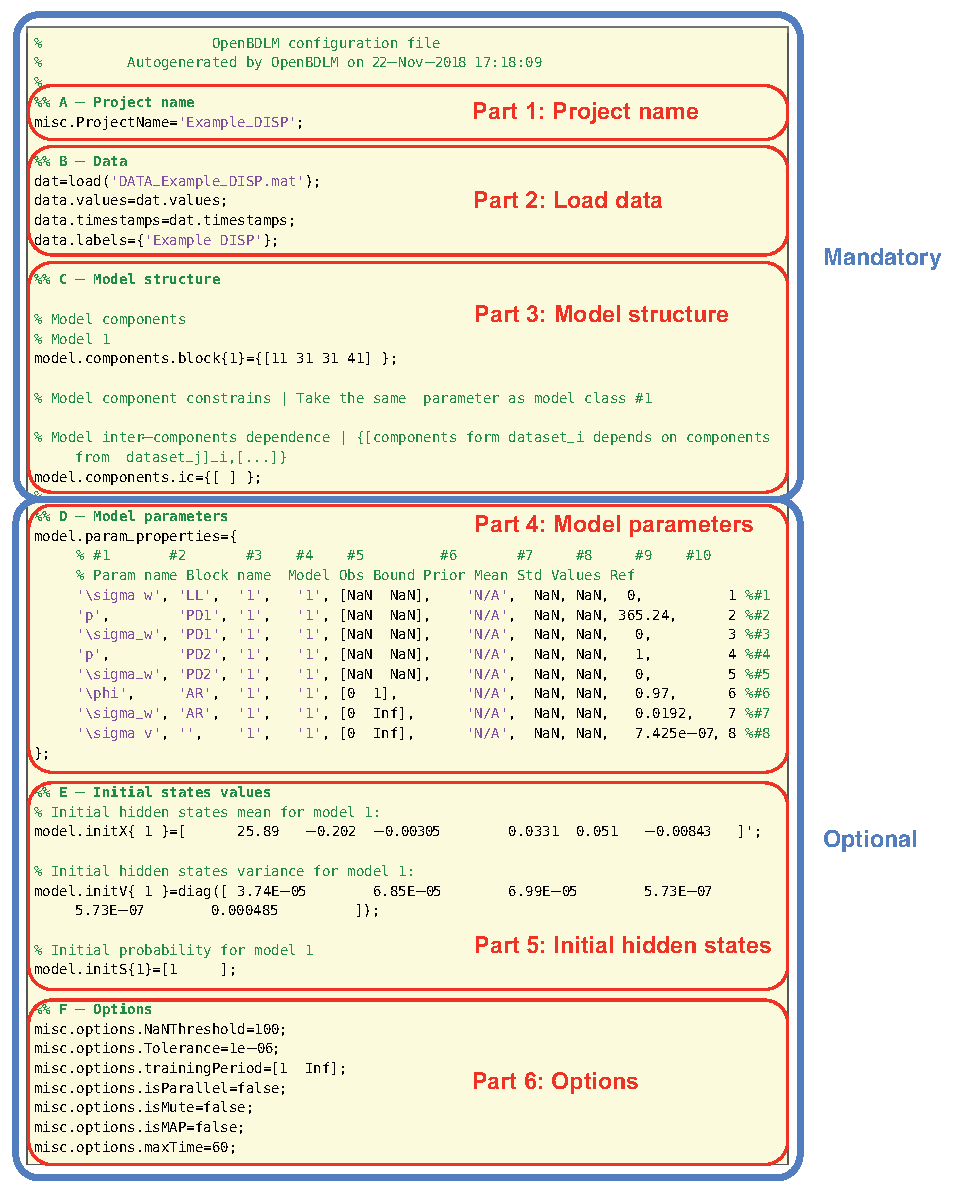
\includegraphics[width=140mm]{docfigs/Example_DISPSIM/listing/config_file_1.pdf}
\caption{Exemple of configuration file}
\label{fig:cfgfile}
\end{figure}

\subsection{Project name}
This section of the configuration file defines the name of the project as a vector of characters stored in the field \lstinline[basicstyle = \mlttfamily \small ]!ProjectName! of the \MATLAB{} variable \lstinline[basicstyle = \mlttfamily \small ]!misc!.

\subsection{Data}

This section of the configuration file defines information required for loading the data from a \lstinline[basicstyle = \mlttfamily \small ]!DATA_! file located in ``/data/mat'' subfolder.
The file must follow the format described in Section~\ref{SS:MATInput}.
The timestamp values, the amplitude values and the label values must be stored in the fields \lstinline[basicstyle = \mlttfamily \small]!timestamps!, \lstinline[basicstyle = \mlttfamily \small]!values!, and \lstinline[basicstyle = \mlttfamily \small]!labels! of the \MATLAB{} structure named \lstinline[basicstyle = \mlttfamily \small]!data!.

\subsection{Model structure}
\label{SS:ModelComponents}
This part of the configuration file defines the model in a \MATLAB{} structure named \lstinline[basicstyle = \mlttfamily \small]!model.component!.
The structure \lstinline[basicstyle = \mlttfamily \small]!model.component! must have three fields, named \lstinline[basicstyle = \mlttfamily \small]!model.component.block!, \lstinline[basicstyle = \mlttfamily \small]!model.component.ic!, and \lstinline[basicstyle = \mlttfamily \small]!model.component.const!.

\begin{itemize}

\item \lstinline[basicstyle = \mlttfamily \small ]!model.component.block!: it defines the block components associated with each time series.
The field \lstinline[basicstyle = \mlttfamily \small ]!block! stores $1\times \mathtt{S}$ cell array, where $\mathtt{S} = \{1,2 \}$ is the number of model classes.
Each cell array is a $1\times \mathtt{D}$ cell array of matrice, where $\mathtt{D}$ is the number of time series.
Each block component is associated with a reference number:
\begin{itemize}
\item 11: Local level 
\item 12: Local trend
\item 13: Local acceleration
\item 21: Local level compatible with local trend
\item 22: Local level compatible with local acceleration
\item 23: Local trend compatible with local acceleration
\item 31: Periodic
\item 41: First-order autoregressive
\item 51: Kernel regression
\item 61: Level intervention
\end{itemize}

\item  \lstinline[basicstyle = \mlttfamily \small ]!model.component.const!: it constrains model parameters between the block components from different model classes.
The field \lstinline[basicstyle = \mlttfamily \small ]!const! stores a $1\times \mathtt{S}$ cell array, where $\mathtt{S} = \{1, 2 \}$ is the total number of model classes.
It is defined only if $\mathtt{S} = 2$.
The first cell is empty, and the second cell is a $1\times \mathtt{D}$ cell array of array, where $\mathtt{D}$ is the number of time series.
The array contains $0$ and $1$ to indicate which block components of the second model class has the same model parameters than the corresponding component of the first model class. 
A value of $1$ indicates that the model parameters are constrained between the block components of the two model classes, $0$ otherwise.

\item  \lstinline[basicstyle = \mlttfamily \small ]!model.component.ic!:  it defines the dependencies among the time series.
The field \lstinline[basicstyle = \mlttfamily \small ]!ic! stores a $1\times \mathtt{D}$ cell array of $1\times (\mathtt{D}-1)$ matrix, where $\mathtt{D}$ is the number of time series.
Each time series depend on the time series corresponding to the indexes given in the $\mathtt{D}$ arrays.
If the array is empty, the time series are considered independent by default.

\end{itemize}


\subsection{Model parameters}
\label{SS:ModelParamProperties}
This part of the configuration file aims at defining the model parameter properties which are stored in the field named \lstinline[basicstyle = \mlttfamily \small ]!model.param_properties! of the \MATLAB{} structure \lstinline[basicstyle = \mlttfamily \small ]!model!.
The field \lstinline[basicstyle = \mlttfamily \small ]!model.param_properties! stores $\mathtt{K} \times 10$ cell array, where $\mathtt{K}$ is the total number of model parameters.
\begin{itemize}
\item column 1 must be a character vector that gives the name of the model parameters (e.g.  \lstinline[basicstyle = \mlttfamily \small ]!sigma_w!). 
\item column 2 must be a character vector that gives the reference name of the block associated with the parameter (e.g \lstinline[basicstyle = \mlttfamily \small ]!LL!, see Section~\ref{SS:BlockComponent}).
\item column 3 must be a character vector that gives the index corresponding to the model class associated with the parameter (e.g  either \lstinline[basicstyle = \mlttfamily \small ]!1! or \lstinline[basicstyle = \mlttfamily \small ]!2!) (see~\ref{SS:THSKF}).
\item column 4 must be a character vector that gives the index corresponding to the observation associated with the parameter (e.g \lstinline[basicstyle = \mlttfamily \small ]!3!).
\item column 5 must be a $1\times2$ array that gives the bound of the parameter (e.g \lstinline[basicstyle = \mlttfamily \small ]![NaN, NaN]!,  \lstinline[basicstyle = \mlttfamily \small ]![0, Inf]!, \lstinline[basicstyle = \mlttfamily \small ]![0, 1]!). 
The bounds are used to transform (if necessary) model parameters from a bounded to  an unbounded space during the optimization process (see Sections~\ref{S:PARAMESTIMATION} and~\ref{SS:THModelParameterEstimation}).
\item column 6 must be a character vector that gives the type of the prior used during the optimization process (e.g  either \lstinline[basicstyle = \mlttfamily \small ]!N/A! or \lstinline[basicstyle = \mlttfamily \small ]!normal!). 
\lstinline[basicstyle = \mlttfamily \small ]!N/A! indicates that no prior is used (see Sections~\ref{S:PARAMESTIMATION} and~\ref{SS:THModelParameterEstimation}).
\item column 7 must be a real number that gives the mean of the prior when a prior of type \lstinline[basicstyle = \mlttfamily \small ]!normal! is used, otherwise it must be set to \lstinline[basicstyle = \mlttfamily \small ]!NaN! (see Sections~\ref{S:PARAMESTIMATION} and~\ref{SS:THModelParameterEstimation}).
\item column 8 must be a real number that gives the standard deviation of the prior when a prior of type \lstinline[basicstyle = \mlttfamily \small ]!normal! is used, otherwise it must be set to \lstinline[basicstyle = \mlttfamily \small ]!NaN! (see Sections~\ref{S:PARAMESTIMATION} and~\ref{SS:THModelParameterEstimation}).
\item column 9 must be a real number that gives the value of the model parameters.
\item column 10 must be an integer that gives the reference number of the model parameters. The model parameters which share the same reference number are constrained to each other.
\end{itemize}

\subsection{Initial states values}
\label{SS:InitialHS}
This part of the configuration file defines the initial states values (at time $t=0$).
The initial mean and covariance hidden states values are stored in the \lstinline[basicstyle = \mlttfamily \small ]!model.initX! and \lstinline[basicstyle = \mlttfamily \small ]!model.initV! fields.
The initial probability for the model class is stored in the field \lstinline[basicstyle = \mlttfamily \small ]!model.initS!.

\begin{itemize}
\item \lstinline[basicstyle = \mlttfamily \small ]!model.initX!: $1\times \mathtt{S}$ cell array of array, where $\mathtt{S} \in \{1, 2 \}$ is the total number of model classes.
Each array is $\mathtt{L}\times1$ array of real number that stores the initial mean values associated with each hidden states variables, where $\mathtt{L}$ is the total number of hidden states variables associated with the model.
\item \lstinline[basicstyle = \mlttfamily \small ]!model.initV!: $1\times \mathtt{S}$ cell array of array, where $\mathtt{S} \in \{1, 2 \}$ is the total number of model classes.
Each array is $\mathtt{L}\times\mathtt{L}$ array of real number that stores the initial variance and covariances values associated with each hidden states variables.
\item \lstinline[basicstyle = \mlttfamily \small ]!model.initS!: $1\times \mathtt{S}$ cell array of array, where $\mathtt{S} \in \{1, 2 \}$ is the total number of model classes. 
Each array is $1\times1$ array of real number that gives the initial probability for the model class.
\end{itemize}

\subsection{Options}
\label{SS:options}
This part of the configuration file defines the options that control different aspect of the software regarding the data pre-processing, optimization, hidden states estimation, and aspects related to graphical outputs.
The options are stored in the field named \text{options} of the \MATLAB{} variable \lstinline[basicstyle = \mlttfamily \small ]!misc!.
\begin{itemize}

\item Options for the data pre-processing

\begin{itemize}
\item \lstinline[basicstyle = \mlttfamily \small ]!misc.options.NaNThreshold!: real number that gives, in percent, the amount of missing data allowed at each time slice.\\Default: \lstinline[basicstyle = \mlttfamily \small ]!100!.
\item \lstinline[basicstyle = \mlttfamily \small ]!misc.options.Tolerance!: real number that gives the duration (in number of days) after which two timestamps are not considered equal. \\Default: $10^{-6}$.

\end{itemize}


\item Options for the model parameters estimation

\begin{itemize}
\item \lstinline[basicstyle = \mlttfamily \small ]!misc.options.trainingPeriod!:  $1\times2$ array of real number that defines the training period, given in number of days since the first timestamp. \\Default: \lstinline[basicstyle = \mlttfamily \small ]![1 Inf]!. 
\item \lstinline[basicstyle = \mlttfamily \small ]!misc.options.isParallel!: logical that triggers or not the parallel computation for approximating the gradient in the optimization procedure. Note that parallel computation requires the \MATLAB{} \emph{Parallel Computing Toolbox}. \\Default: \lstinline[basicstyle = \mlttfamily \small ]!true!.
\item \lstinline[basicstyle = \mlttfamily \small ]!misc.options.maxIterations!: integer that gives the maximum number of iterations for the optimization procedure. Newton-Raphson only. \\Default: \lstinline[basicstyle = \mlttfamily \small ]!100!.
\item \lstinline[basicstyle = \mlttfamily \small ]!misc.options.maxTime!: real number that gives, in minutes, the maximum amount of  time to spend for the optimization procedure. \\Default: \lstinline[basicstyle = \mlttfamily \small ]!60!.
\item \lstinline[basicstyle = \mlttfamily \small ]!misc.options.isMAP!: logical that triggers or not the Maximum A Posteriori (MAP) estimation of the model parameters during the optimization procedure. MAP estimation includes prior information about the model parameters. \\Default: \lstinline[basicstyle = \mlttfamily \small ]!false!.
\item \lstinline[basicstyle = \mlttfamily \small ]!misc.options.isPredCap!: logical so that if \lstinline[basicstyle = \mlttfamily \small ]!isPredCap=true!, the Prediction Capacity (i.e. the log-likelihood over a test dataset) is used to drive the optimization process, otherwise the log-likelihood over the full dataset is used. This option is used only for Stochastic Gradient optimization. \\Default: \lstinline[basicstyle = \mlttfamily \small ]!false!.
\item \lstinline[basicstyle = \mlttfamily \small ]!misc.options.isLaplaceApprox!: logical so that if \lstinline[basicstyle = \mlttfamily \small ]!isLaplaceApprox=true! the posterior covariance matrix is estimated using Laplace approximation around the optimized model parameters values. This option is used only for Newton-Raphson optimization. \\Default: \lstinline[basicstyle = \mlttfamily \small ]!false!.
\item \lstinline[basicstyle = \mlttfamily \small ]!misc.options.NRTerminationTolerance!: real value determining the termination tolerance for the Newton-Raphson algorithm. \\Default: $10^{-7}$.
\item \lstinline[basicstyle = \mlttfamily \small ]!misc.options.NRLevelsLambdaRef!: integer that controls the number of trial loop for a parameter being optimized for theNewton-Raphson algorithm. \\Default: $4$.
\item \lstinline[basicstyle = \mlttfamily \small ]!misc.options.isMute!: logical so that if \lstinline[basicstyle = \mlttfamily \small ]!isMute=true!, no message are displayed on screen during the optimization procedure. \\Default: \lstinline[basicstyle = \mlttfamily \small ]!false!.
\item \lstinline[basicstyle = \mlttfamily \small ]!misc.options.maxEpochs!: integer that gives the maximum number of epochs the optimization procedure. This option is used only for Stochastic Gradient optimization. \\Default: \lstinline[basicstyle = \mlttfamily \small ]!50!.
\item \lstinline[basicstyle = \mlttfamily \small ]!misc.options.Optimizer!: vector of character that defines the optimizer for Stochastic Gradient algorithm. It must be either \lstinline[basicstyle = \mlttfamily \small ]!'MMT'!, \lstinline[basicstyle = \mlttfamily \small ]!'ADAM'!, \lstinline[basicstyle = \mlttfamily \small ]!'MMTbeta'!, \lstinline[basicstyle = \mlttfamily \small ]!'ADAMbeta'!. This option is used only for Stochastic Gradient optimization. \\Default: \lstinline[basicstyle = \mlttfamily \small ]!'MMT'!.
\item \lstinline[basicstyle = \mlttfamily \small ]!misc.options.SplitPercent!: real number that defines defines in percent the portion of the training data used for validation. \\Default: \lstinline[basicstyle = \mlttfamily \small ]!30!.
\item \lstinline[basicstyle = \mlttfamily \small ]!misc.options.MiniBatchSizePercent!: real number that defines defines the size of mini-batch, in percent of the training data. \\Default: \lstinline[basicstyle = \mlttfamily \small ]!20!.
\item \lstinline[basicstyle = \mlttfamily \small ]!misc.options.SGTerminationTolerance!: termination tolerance for the Stochastic gradient algorithm. This option is used only for Stochastic Gradient optimization. \\Default: \lstinline[basicstyle = \mlttfamily \small ]!0.95!.
\end{itemize}

\item Options for the estimation

\begin{itemize}
\item \lstinline[basicstyle = \mlttfamily \small ]!misc.options.MaxSizeEstimation!: real number that gives the maximum size, in Mb, for which the hidden states estimations are saved in the \lstinline[basicstyle = \mlttfamily \small ]!PROJ_! file at the end of the analysis. \\Default: \lstinline[basicstyle = \mlttfamily \small ]!100!.
\item \lstinline[basicstyle = \mlttfamily \small ]!misc.options.MethodStateEstimation!: vector of character. It must be either \lstinline[basicstyle = \mlttfamily \small ]!'kalman'! or \lstinline[basicstyle = \mlttfamily \small ]!'UD'!. it gives the method used for the estimation of the hidden states. \\Default: \lstinline[basicstyle = \mlttfamily \small ]!'kalman'!.
\item \lstinline[basicstyle = \mlttfamily \small ]!misc.options.DataPercent!: real number that gives in percent the amount of data, starting at $t=1$ used for the estimation of the initial hidden states. \\Default: \lstinline[basicstyle = \mlttfamily \small ]!100!.
\item \lstinline[basicstyle = \mlttfamily \small ]!misc.options.KRNumberControlPoints!: integer that gives the number of control points used for the periodic kernel regression component (see Section~\ref{SS:BlockComponent}). \\Default: \lstinline[basicstyle = \mlttfamily \small ]!100!.
\end{itemize}


\item Options for the synthetic data creation

\begin{itemize}
\item \lstinline[basicstyle = \mlttfamily \small ]!misc.options.Seed!: integer that controls the random number generation used to create synthetic data. Synthetic data created with the same seed are identical (useful to replicate results). If  \lstinline[basicstyle = \mlttfamily \small ]!misc.options.Seed=[]!, the seed is based on current time and therefore, a different sequence of random number  is generated at each run. \\Default: \lstinline[basicstyle = \mlttfamily \small ]!12345!.
\end{itemize}

\item Options for the graphical outputs

\begin{itemize}
\item \lstinline[basicstyle = \mlttfamily \small ]!misc.options.isPlotEstimations!: logical. if \lstinline[basicstyle = \mlttfamily \small ]!isPlotEstimations=true!, figures plotting the estimation results popup on screen each time the hidden states are estimated. \\Default: \lstinline[basicstyle = \mlttfamily \small ]!true!.
\item \lstinline[basicstyle = \mlttfamily \small ]!misc.options.FigurePosition!: $1\times4$ array of real number that gives the location and size of the drawable area, specified as a vector of the form [left bottom width height] in the current units of \MATLAB{}. \\Default: \lstinline[basicstyle = \mlttfamily \small ]![100, 100, 1300, 270]!
\item \lstinline[basicstyle = \mlttfamily \small ]!misc.options.isSecondaryPlot!: logical. if \lstinline[basicstyle = \mlttfamily \small ]!isSecondaryPlot=true!, a closeup over two weeks is plotted at the right of each figure. \\Default: \lstinline[basicstyle = \mlttfamily \small ]!false!.
\item \lstinline[basicstyle = \mlttfamily \small ]!misc.options.Subsample!: integer that controls the number of points that are displayed in the plots. The number of points to plot is divided by a factor given by the values of \lstinline[basicstyle = \mlttfamily \small ]!misc.options.Subsample!. \\Default: \lstinline[basicstyle = \mlttfamily \small ]!1!.
\item \lstinline[basicstyle = \mlttfamily \small ]!misc.options.Linewidth!: real number that controls the width of the line plotted in the figure. \\Default: \lstinline[basicstyle = \mlttfamily \small ]!1!.
\item \lstinline[basicstyle = \mlttfamily \small ]!misc.options.ndivx!: integer that controls the number of labels for abscissa x-axis in each figure. \\Default: \lstinline[basicstyle = \mlttfamily \small ]!4!.
\item \lstinline[basicstyle = \mlttfamily \small ]!misc.options.ndivy!: integer that controls the number of labels for ordinate y-axis in each figure. \\Default: \lstinline[basicstyle = \mlttfamily \small ]!3!.
\item \lstinline[basicstyle = \mlttfamily \small ]!misc.options.Xaxis_lag!: real number that gives in number of days the amount of time by which the x-axis is shifted on each figure. \\Default: \lstinline[basicstyle = \mlttfamily \small ]!0!. 
\item \lstinline[basicstyle = \mlttfamily \small ]!misc.options.isExportTEX!: logical so that if \lstinline[basicstyle = \mlttfamily \small ]!isExportTEX=true!, figures are exported in \LaTeX{} format. \\Default: \lstinline[basicstyle = \mlttfamily \small ]!false!.
\item \lstinline[basicstyle = \mlttfamily \small ]!misc.options.isExportPNG!: logical so that if \lstinline[basicstyle = \mlttfamily \small ]!isExportPNG=true!,  figures are exported in PNG format. \\Default: \lstinline[basicstyle = \mlttfamily \small ]!false!.
\item \lstinline[basicstyle = \mlttfamily \small ]!misc.options.isExportPDF!: logical so that if \lstinline[basicstyle = \mlttfamily \small ]!isExportPDF=true!,  figures are exported in PDF format. \\Default: \lstinline[basicstyle = \mlttfamily \small ]!false!.
\end{itemize}
\end{itemize}\clearpage

\section{OpenBDLM workflow}
\label{S:WORKFLOW}

%\begin{figure}[!h]
\begin{sidewaysfigure}
  \centering
  \captionsetup{justification=centering}
\scalebox{0.8}{
\begin{tikzpicture}

% Node position
\node[paraamber](rawdata){\begin{tabular}{c}  .MAT \\ and \\ .CSV data files \end{tabular}};
\node[esamber, below of=rawdata, yshift=-1.3cm] (preprocess) {\begin{tabular}{c}  pre- \\   processing \end{tabular} };
\node[test, below of=preprocess,  yshift=-1.3cm] (testpreprocess) {? };
\node[esbisque, right of=testpreprocess, xshift = 1.75cm ] (configmodel) {  \begin{tabular}{c}  model \\  configuration \end{tabular} };
\node[esbisque, right of=configmodel, xshift = 1.75cm ] (buildmodel) {   \phantom{} build model \phantom{} };
\node[esbabyblueeyes, right of=buildmodel, xshift=1.75cm] (paramlearning){\begin{tabular}{c}   parameters \\  learning \end{tabular}};
\node[parawhite, below of=paramlearning, xshift=0cm, yshift = -1.5cm] (inputcfg){\begin{tabular}{c}  CFG\_*.m \\  DATA\_*.mat \end{tabular}};
\node[test, right of=paramlearning, xshift = 1.5cm] (testparamlearning) {?};
\node[esceladon, right of=testparamlearning, xshift = 1.5cm] (stateestimation) {\begin{tabular}{c}   states \\   estimation \end{tabular}};
\node[test, right of=stateestimation, xshift = 1.5cm] (teststateestimation) {?};
\node[parawhite, right of=teststateestimation, xshift = 2.25cm] (results) {\begin{tabular}{c}  CFG\_*.m  \\  DATA\_*.mat \\ RES\_*.mat \\ PROJ\_*.mat \\  LOG\_*.txt  \end{tabular}};
\node[user, below of=testpreprocess, yshift=-2.5cm] (user1) { \includegraphics[height=0.45cm]{./docfigs/user_logo.png}};
\node[user, below of=configmodel, yshift=-2.5cm] (user2) { \includegraphics[height=0.45cm]{./docfigs/user_logo.png}};
\node[user, below of=testparamlearning, yshift=-2.5cm] (user3) { \includegraphics[height=0.45cm]{./docfigs/user_logo.png}};
\node[user, below of=teststateestimation, yshift=-2.5cm] (user4) { \includegraphics[height=0.45cm]{./docfigs/user_logo.png}};
\node[eslightgray, above of=paramlearning, yshift=4cm, xshift=0cm](syntheticdatacreation) {\phantom{} synthetic data creation \phantom{}};

 % Define path
\path[->, thick]  (rawdata)edge(preprocess);
\path[-, thick]  (preprocess)edge(testpreprocess);
\path[<->, thick]  (testpreprocess)edge(user1);
\path[-, thick]  (configmodel)edge(buildmodel);
\path[<->, thick]  (configmodel)edge(user2);
\path[-, thick]  (buildmodel)edge(paramlearning);
\path[-, thick]  (paramlearning)edge(testparamlearning);
\path[<->, thick]  (testparamlearning)edge(user3);
\path[-, thick]  (testparamlearning)edge(stateestimation);
\path[-, thick] (stateestimation) edge (teststateestimation);
\path[<->, thick]  (teststateestimation)edge(user4);
\path[-, thick] (testpreprocess) edge node[anchor=center, above] { yes}  (configmodel);
\path[->, draw, thick] (testpreprocess.west) -| (-1.25cm,-3cm) |- node[anchor=center, above, rotate=90, fill=none]{ no} (preprocess.west);
\path[->, thick] (teststateestimation) edge node[anchor=center, above] { yes}  (results);
\path[->, draw, thick] (testparamlearning.north) |- (9cm,-2.5cm) -| node[anchor=center, above, rotate=0, fill=none]{ no} (paramlearning.north);
\path[-, draw, thick] (testparamlearning)  edge node[anchor=center, above] { yes}  (stateestimation);
\path[->, draw, thick] (teststateestimation.north) |- (6cm,-2cm) -| node[anchor=center, above, rotate=0, fill=none]{ no} (buildmodel.north);
\path[->, draw, thick] (inputcfg) edge (paramlearning);

\path[->, draw, thick, dashed] (buildmodel.east) -| (6.75cm, -0.75cm) -| (syntheticdatacreation.south);
\path[->, draw, thick, dashed] (paramlearning.east) -| (9.75cm, -0.75cm) -| (syntheticdatacreation.south);
\path[->, draw, thick, dashed] (stateestimation.east) -| (14.5cm, -0.75cm) -| (syntheticdatacreation.south);
\path[->, draw, thick, dashed] (syntheticdatacreation.north) |- (9cm, 2cm) -| (rawdata.north);
\path[->, draw, thick, dashed] (syntheticdatacreation.north) |- (18cm, 2cm) -| (results.north);

 % Rectangle
\draw [draw=amber, line width=0.5mm, dashed ] (-3cm, -3cm) rectangle ++(5cm , 4cm );
\draw [draw=bisque, line width=0.5mm, dashed ] (0.95cm,-5.55cm) rectangle ++(5.85cm , 2cm );
\draw [draw=babyblueeyes, line width=0.5mm, dashed ] (7cm,-5.55cm) rectangle ++(2.5cm , 2cm );
\draw [draw=celadon, line width=0.5mm, dashed ] (11.85cm,-5.55cm) rectangle ++(2.75cm , 2cm );
\draw [draw=lightgray, line width=0.5mm, dashed ] (6cm,-0.5cm) rectangle ++(4.5cm , 1.75cm );
 
 % Text
\node[ above of = rawdata, xshift = -0.5cm, yshift = 0.325 cm, fill=white] { Section~\ref{S:DATALOADING} and~\ref{S:DATAEDITINGPREPROCESSING}};
\node[ above of = buildmodel, xshift = -1cm, yshift = 0.325 cm, fill=white] { Section~\ref{S:MODELCONFIGURATION} and~\ref{S:MODELCONSTRUCTION}};
\node[above of = paramlearning, xshift = 0cm, yshift = 0.325 cm,  fill=white] { Section~\ref{S:PARAMESTIMATION} };
\node[above of = stateestimation, xshift = 0cm, yshift = 0.325 cm,  fill=white] { Section~\ref{S:HIDDENSTATESESTIMATION} };
\node[above of = syntheticdatacreation, xshift = 0cm, yshift = 0.325 cm,  fill=white] { Section~\ref{S:SYNTHETIC}};



\end{tikzpicture} }
\caption{OpenBDLM workflow} \label{FIG:OpenBDLMworkflow}
%\end{figure}
\end{sidewaysfigure}\clearpage

\section{Generate synthetic data}
\label{S:SYNTHETIC}
The creation of synthetic data is possible using OpenBDLM.
The analysis of synthetic data is useful for validation, test, and debugging purposes because the true value of the hidden states and model parameters are known.
OpenBDLM uses the transition model  of the state-space modelling approach (see Section~\ref{SS:LGSSM}) to create realistic synthetic data.
There are two ways for creating synthetic data using OpenBDLM:

\begin{itemize}
\item From the interactive tool
\item From an existing project.
\end{itemize}

\subsection{Generate synthetic data using the interactive tool}
The creation of the synthetic data from the interactive tool (option \colorbox{light-gray}{\lstinline[basicstyle = \mlttfamily \small, backgroundcolor = \color{light-gray}]!0!} from the starting menu) enables the creation of synthetic data from scratch. 
OpenBDLM requests the user to provide the number of time series, and to define the time vector (starting time, end time, timestep).
In the next step, the user has to define the time-series dependence (if applicable), to provide the number of model class, and to define a set of block components for each time series, as well as model constrains between model classes (if applicable).
Default values for initial hidden states mean values and model parameters are automatically assigned for each block component.
In the case of two model classes, the synthetic baseline will switch between the first and the second model class according to the transition probability values (see Section~\ref{SS:THSKF}).
The amplitude of each synthetic anomaly (i.e. change of the local trend) is sampled randomly in a normal distribution of zero mean and standard deviation $\sigma_{w}^{12}$ as defined in the switching process noise transition matrix.
Alternately, the user may choose to create \emph{custom anomalies}.
In such a case, the beginning (in sample index), duration (in number of samples) and amplitude (in change of the local trend) of each anomaly is user specified.
The information about custom anomaly are stored in the field \lstinline[basicstyle = \mlttfamily \small, backgroundcolor = \color{light-gray}]!custom_anomalies! of the structure variable \lstinline[basicstyle = \mlttfamily \small, backgroundcolor = \color{light-gray}]!misc!:
\begin{itemize}
\item \lstinline[basicstyle = \mlttfamily \small, backgroundcolor = \color{light-gray}]!misc.custom_anomalies.start_custom_anomalies!: this field stores a $1\times \mathtt{A}$ vector of integers, where $\mathtt{A}$ is the total number of synthetic anomaly. Each value indicates the sample index of the anomaly start.
\item \lstinline[basicstyle = \mlttfamily \small, backgroundcolor = \color{light-gray}]!misc.custom_anomalies.duration_custom_anomalies!: this field stores a $1\times \mathtt{A}$ vector of integers, where $\mathtt{A}$ is the total number of synthetic anomaly. Each value indicates the anomaly duration in number of samples.
\item \lstinline[basicstyle = \mlttfamily \small, backgroundcolor = \color{light-gray}]!misc.custom_anomalies.amplitude_custom_anomalies!: this field stores a $1\times \mathtt{A}$ vector of real number, where $\mathtt{A}$ is the total number of synthetic anomaly. Each value indicates the amplitude of the anomaly in change of the local trend.
\end{itemize}
The synthetic data are saved in \lstinline[basicstyle = \mlttfamily \small, backgroundcolor = \color{light-gray}]!DATA_*.mat! and \lstinline[basicstyle = \mlttfamily \small, backgroundcolor = \color{light-gray}]!*.csv! data files, and a \lstinline[basicstyle = \mlttfamily \small, backgroundcolor = \color{light-gray}]!PROJ_*.mat! project file is created that stores the information about the model (structure variable \lstinline[basicstyle = \mlttfamily \small, backgroundcolor = \color{light-gray}]!model!), and the true hidden states (see structure variable \lstinline[basicstyle = \mlttfamily \small, backgroundcolor = \color{light-gray}]!estimation.ref!).





\begin{table}[h]
     \caption{Default value of model parameters and initial hidden states $\bm{\mu}_{0}$ and $\mathbf{\Sigma}_{0}$ for synthetic data generation.} 
     \centering
     \begin{tabular}{r|lp{3.1cm}p{4cm}}\toprule
        & $\bm{\theta}$ & $\bm{\mu}_{0}$ & diag$(\mathbf{\Sigma}_{0})$ \\\cmidrule(lr){1-4}
    $\mathtt{LL}$   &  $\sigma_{w}^{\mathtt{LL}}=0$ &$[10]$ & $[0.1^{2}]$ \\
    $\mathtt{LT}$    & $\sigma_{w}^{\mathtt{LT}}=10^{-7}$ &  $[10, -0.1\times10^{-2}]$ & $[0.1^{2}, 0.1^{2}]$ \\
     $\mathtt{LA}$   & $\sigma_{w}^{\mathtt{LA}}=10^{-8}$  &  $[10, -0.1\times10^{-2} , -0.1\times10^{-5}]$ & $[0.1^{2}, 0.1^{2}, 0.1^{2}]$ \\
     $\mathtt{P}$  &  $p=[365.24, 1, 182.62] $, $\sigma_{w}^{\mathtt{P}}=0$  &$[10, 10]$ & $[0.2^{2}, 0.2^{2}]$  \\
     $\mathtt{KR}$  & $p=[365.24]$, $\ell=0.5$, $\sigma_{w,0}^{\mathtt{KR}}=\sigma_{w,1}^{\mathtt{KR}}=0$ &  $[$$-0.97$, $1.65$, $1.73$, $-1.91$, $0.23$, $0.37$, $-2.89$, $-0.22$, $0.73$, $-1.83$$]$ & $[$$0.01^{2}$, $0.01^{2}$, $0.01^{2}$, $0.01^{2}$, $0.01^{2}$, $0.01^{2}$, $0.01^{2}$, $0.01^{2}$, $0.01^{2}$, $0.01^{2}$$]$  \\  
         $\mathtt{AR}$   &  $\phi^{\mathtt{AR}}=0.75$, $\sigma_{w}^{\mathtt{AR}}=1$  &$[0]$ & $[0.1^{2}]$ \\\bottomrule
     \end{tabular}
\label{table:defaultsynthetic}
\end{table}

\subsection{Generate synthetic data from an existing project}



Once a project is loaded, it is possible to create synthetic data from it (option \colorbox{light-gray}{\lstinline[basicstyle = \mlttfamily \small, backgroundcolor = \color{light-gray}]!16!} from the main menu (see Listing~\ref{LST:OpenBDLMMainMenu}).
The synthetic data time vector will be the same as the time vector in memory, and missing data will be replicated.
The model used to create the synthetic data will be the same as the model of the current project, including current initial hidden states as well as model parameters values.
The creation of synthetic data in this way is particularly useful to closely mimic real dataset.
The synthetic data are saved in \lstinline[basicstyle = \mlttfamily \small, backgroundcolor = \color{light-gray}]!DATA_new_*.mat! and \lstinline[basicstyle = \mlttfamily \small, backgroundcolor = \color{light-gray}]!*.csv! data files, and a \lstinline[basicstyle = \mlttfamily \small, backgroundcolor = \color{light-gray}]!PROJ_new_*.mat! new project file is created that stores the information about the model (structure variable \lstinline[basicstyle = \mlttfamily \small, backgroundcolor = \color{light-gray}]!model!), and the true hidden states (see structure variable \lstinline[basicstyle = \mlttfamily \small, backgroundcolor = \color{light-gray}]!estimation.ref!).






\subsection{Synthetic data generation functions}


The synthetic data creation workflow is presented Figure~\ref{FIG:SyntheticDataCreationWorkflow}. 
The OpenBLDM functions used for synthetic data creation are:

\begin{description}[style=unboxed]\setlength\itemsep{0em}
\item[Pilot function for synthetic data creation] \leavevmode
  \begin{lstlisting}[ basicstyle = \mlttfamily \small, breaklines=true]
[data,model,estimation,misc]=piloteSimulateData(data,model,estimation,misc)
  \end{lstlisting}

\item[Creates synthetic data] \leavevmode
  \begin{lstlisting}[ basicstyle = \mlttfamily \small, breaklines=true]
[data,model,estimation,misc]=SimulateData(data,model,misc,varargin)
  \end{lstlisting}

\item[Create synthetic data from transition probabilities] \leavevmode
  \begin{lstlisting}[ basicstyle = \mlttfamily \small, breaklines=true]
[data, model, estimation, misc]=simulateDataFromTransitionProbabilities(data,model,misc)
  \end{lstlisting}

\item[Create synthetic data from custom anomalies (for two model classes only)] \leavevmode
  \begin{lstlisting}[ basicstyle = \mlttfamily \small, breaklines=true]
[data,model,estimation,misc]=simulateDataFromCustomAnomalies(data,model,misc)
  \end{lstlisting}

  \item[Models configuration for synthetic data (for synthetic data creation from interactive tool only)] \leavevmode
  \begin{lstlisting}[ basicstyle = \mlttfamily \small, breaklines=true]
[data,model,estimation,misc]=configureModelForDataSimulation(data,model,estimation,misc)
 \end{lstlisting}
 
 \item[Requests user inputs to define the number of synthetic time series to create (for synthetic data creation from interactive tool only)] \leavevmode
  \begin{lstlisting}[ basicstyle = \mlttfamily \small, breaklines=true]
  [data,misc]=defineDataLabels(data,misc)
 \end{lstlisting}
 
\item[Requests user inputs to define synthetic data time vector (for synthetic data creation from interactive tool only)] \leavevmode
  \begin{lstlisting}[ basicstyle = \mlttfamily \small, breaklines=true]
[data,misc]=defineTimestamps(data,misc)
 \end{lstlisting}

\end{description}



\begin{figure}[h]
  \centering
  \captionsetup{justification=centering}
\scalebox{0.7}{
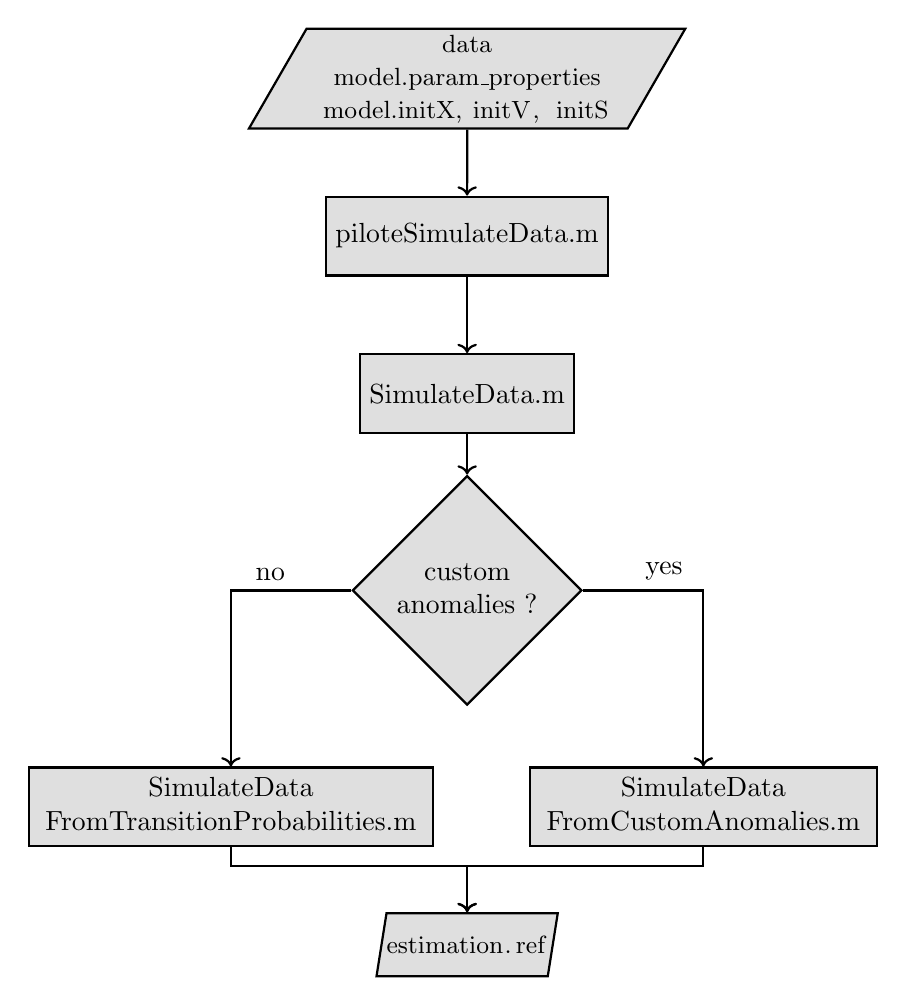
\begin{tikzpicture}

\node[paralightgray](inputSDC){\begin{tabular}{c}  \lstinline[ basicstyle = \mlttfamily \small]!data! \\ \lstinline[ basicstyle = \mlttfamily \small]!model.param_properties! \\ \lstinline[ basicstyle = \mlttfamily \small]!model.initX, initV, initS! \end{tabular}};
\node[eslightgray](piloteSDC)[below of = inputSDC, yshift = -1cm]{\phantom{} piloteSimulateData.m \phantom{}};
\node[eslightgray](SDC)[below of = piloteSDC, yshift = -1cm]{\phantom{} SimulateData.m \phantom{}};
\node[testlightgray](testCustom)[below of = SDC, yshift = -1.5cm]{\begin{tabular}{c}  custom  \\ anomalies ?  \end{tabular}};
\node[eslightgray](SDCtransition)[below of = testCustom, yshift = -1.75cm, xshift = -3cm]{\begin{tabular}{c} SimulateData \\ FromTransitionProbabilities.m \end{tabular}};
\node[eslightgray](SDCcustom)[below of = testCustom , yshift = -1.75cm, xshift = 3cm]{\begin{tabular}{c} SimulateData \\ FromCustomAnomalies.m \end{tabular}};
\node[paralightgray](outputSDC)[below of = inputSDC, yshift = -10cm]{\lstinline[ basicstyle = \mlttfamily \small]!estimation.ref!};
%
\path[->, draw, thick] (inputSDC)edge(piloteSDC);
\path[->, draw, thick] (piloteSDC)edge(SDC);
\path[->, draw, thick] (SDC)edge(testCustom);
\path[->, draw, thick] (testCustom.east) -| (2cm,-6.5cm) -| node[pos=0.25, above]{yes} (SDCcustom);
\path[->, draw, thick] (testCustom.west) -| (-2cm,-6.5cm) -| node[pos=0.25, above]{no} (SDCtransition);
\path[->, draw, thick] (SDCtransition.south) |- (0cm,-10cm) -|  (outputSDC.north);
\path[->, draw, thick] (SDCcustom.south) |- (0cm,-10cm) -|  (outputSDC.north);
\end{tikzpicture} } 
\caption{Synthetic data creation workflow} \label{FIG:SyntheticDataCreationWorkflow}
\end{figure}\clearpage

\section{Results}

\subsection{Visualizing results}
\label{S:VisualizingResults}

The figures that popup on screen aim to represent the data, the data summary, and the hidden states results for each step of the analysis.
Note that in contrast with the data plot, the data summary plot offers a way  to visualize the amplitude, the timesteps and the data availability in a compact way.
By default, a solid line connects two successive real-valued measurement, whatever the timestep.
Missing data (NaN) are not represented in the plot of the observed data, thus resulting in gap for large period  of time with missing data.
The data availability in the data summary plot indicates each missing data with a red cross, thus making it useful to detect sparse missing data which are invisible in the data amplitude plots.
The working period of the sensor is represented by a thick green line in the data availability plot.
The plot appearance may be controlled from the dedicated \lstinline[basicstyle = \mlttfamily \small]!misc.options!.

\subsubsection{Generating figures at any time}
The option \colorbox{light-gray}{\lstinline[basicstyle = \mlttfamily \small]!14!} from the main menu allows generating the different type of figure at any time (see~\ref{LST:PlotMenu}).

\subsubsection{Saving figures}
It is not advised to save figures ``manually'' using the Matlab.
It would most likely not save figures as seen on the screen.
Instead, use the OpenBDLM export facilities described in the Section~\ref{SS:ExportResults}, or set the \lstinline[basicstyle = \mlttfamily \small]!misc.options.isExportTEX!, \lstinline[basicstyle = \mlttfamily \small]!misc.options.isExportPDF!, \lstinline[basicstyle = \mlttfamily \small]!misc.options.isExportPDF! to \lstinline[basicstyle = \mlttfamily \small]!true! to automatically save the figure in a specific format each time a figure is created \footnote{Automatic figure saving is not recommanded because it is computationally expensive.}.
The workflow for visualization is shown in Figure~\ref{FIG:ResultsVisualizationsWorkflow}. 
The functions used to visualize the data and results are:

\begin{lstlisting}[ frame = single, basicstyle = \mlttfamily \small, caption = {OpenBDLM plot menu}, label = LST:PlotMenu ,  float =ht, linewidth=\linewidth, captionpos=b]
----------------------------
/    Plot
----------------------------

     1 ->  Plot data 
     2 ->  Plot data summary 
     3 ->  Plot hidden states 

     Type R to return to the previous menu

     choice >> 
\end{lstlisting}



\begin{description}[style=unboxed]
\item[Pilote function to plot data and estimations] \leavevmode
  \begin{lstlisting}[ basicstyle = \mlttfamily \small, breaklines=true]
  [misc] = pilotePlot(data,model,estimation,misc)
 \end{lstlisting}

\item[Plot data amplitude values and data timestep] \leavevmode
  \begin{lstlisting}[ basicstyle = \mlttfamily \small, breaklines=true]
[FigureNames] = plotData(data,misc,varargin)
 \end{lstlisting}

\item[Plot data amplitude, data time step, and data availability ]  \leavevmode
  \begin{lstlisting}[ basicstyle = \mlttfamily \small, breaklines=true]
  plotDataSummary(data, misc, varargin)
 \end{lstlisting}

 \item[Plot hidden states, predicted data, and model probability]  \leavevmode
  \begin{lstlisting}[ basicstyle = \mlttfamily \small, breaklines=true]
plotEstimations(data,model,estimation,misc,varargin)
 \end{lstlisting}
 
  \item[Plot true and estimated hidden states]  \leavevmode
  \begin{lstlisting}[ basicstyle = \mlttfamily \small, breaklines=true]
  [FigureNames] = plotHiddenStates(data,model,estimation,misc,varargin)
 \end{lstlisting}
 
   \item[Plot observed and predicted data]  \leavevmode
  \begin{lstlisting}[ basicstyle = \mlttfamily \small, breaklines=true]
  [FigureNames] = plotPredictedData(data,model,estimation,misc,varargin)
 \end{lstlisting}
 
    \item[Plot true and estimated model probability]  \leavevmode
  \begin{lstlisting}[ basicstyle = \mlttfamily \small, breaklines=true]
  [FigureNames] = plotModelProbability(data,model,estimation,misc,varargin)
 \end{lstlisting}
 
     \item[Waterfall plot for kernel regression component]  \leavevmode
  \begin{lstlisting}[ basicstyle = \mlttfamily \small, breaklines=true]
[FigureNames] = plotWaterfallKRegression(data,model,estimation,misc,varargin)
 \end{lstlisting}
 
 \item[Export the current figure in TeX (tikz) file using matlab2tikz]  \leavevmode
  \begin{lstlisting}[ basicstyle = \mlttfamily \small, breaklines=true]
 exportPlot(FigureName,varargin)
 \end{lstlisting}
 
\end{description}


\begin{figure}[!h]
  \centering
  \captionsetup{justification=centering}
\scalebox{0.8}{
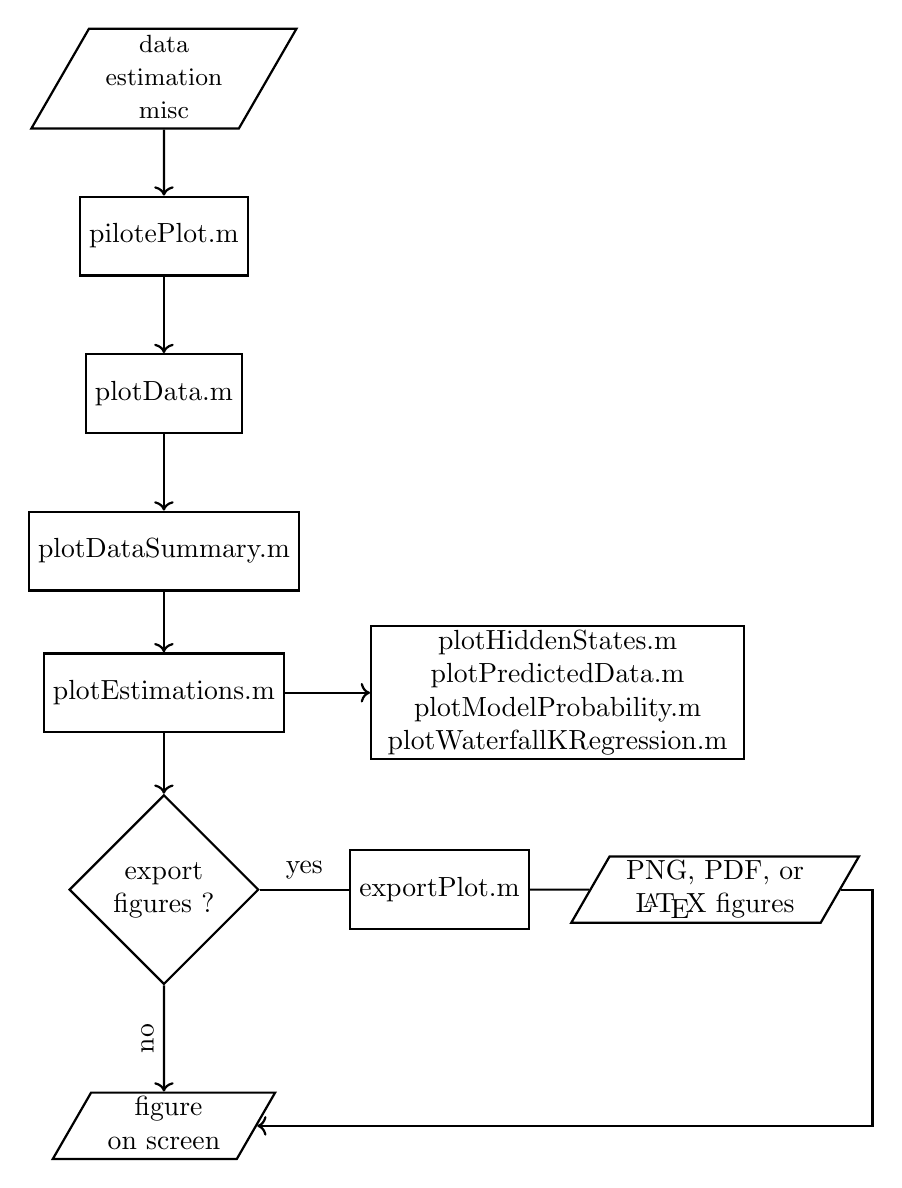
\begin{tikzpicture}

\node[parawhite](inputResultsVisualization){\begin{tabular}{c} \lstinline[basicstyle = \mlttfamily \small ]!data!  \\ \lstinline[basicstyle = \mlttfamily \small ]!estimation! \\ \lstinline[basicstyle = \mlttfamily \small ]!misc!  \end{tabular}};
\node[eswhite](pilote)[below of = inputResultsVisualization, yshift=-1cm, xshift = 0cm]{ \phantom{} pilotePlot.m \phantom{} };
\node[eswhite](plotData)[below of = pilote, yshift=-1cm, xshift = 0cm]{ \phantom{} plotData.m \phantom{} };
\node[eswhite](plotDataSummary)[below of = plotData, xshift = 0cm, yshift=-1cm, ]{ \phantom{} plotDataSummary.m \phantom{} };
\node[eswhite](plotEstimations)[below of = plotDataSummary, yshift= -0.8cm]{\phantom{} plotEstimations.m \phantom{}};
\node[eswhite](plotAll)[right of = plotEstimations, yshift= 0cm, xshift = 4cm]{\begin{tabular}{c} plotHiddenStates.m \\ plotPredictedData.m \\ plotModelProbability.m \\ plotWaterfallKRegression.m  \end{tabular}};
\node[testwhite](testExport)[below of = plotEstimations, yshift= -1.5cm, xshift = 0cm]{\begin{tabular}{c} export \\ figures ?  \end{tabular}};
\node[eswhite](Export)[right of = testExport , yshift=0cm, xshift = 2.5cm]{ \phantom{}  exportPlot.m \phantom{} };
\node[parawhite](outputExport)[right of = Export , yshift=0cm, xshift = 2.5cm]{ \begin{tabular}{c} PNG, PDF, or \\ \LaTeX{} figures \end{tabular}};
\node[parawhite](outputResultsVisualization1)[below of =testExport, yshift=-2cm, xshift = 0cm]{\begin{tabular}{c}  \MATLAB{} figure \\ on screen  \end{tabular}};

\path[->, thick] (inputResultsVisualization)edge(pilote);
\path[->, thick] (pilote)edge(plotData);
\path[->, thick] (plotData)edge(plotDataSummary);
\path[->, thick] (plotDataSummary)edge(plotEstimations);
\path[->, thick] (plotEstimations)edge(plotAll);
\path[->, thick] (plotEstimations)edge(testExport);
\path[-, thick] (testExport)edge  node[anchor=center, above, rotate=0, rotate=0]{ yes}  (Export);
\path[-, thick] (Export)edge(outputExport);
\path[->, thick] (testExport)edge node[anchor=center, above, rotate=0, rotate=90]{ no}  (outputResultsVisualization1);
\path[->, draw,  thick] (outputExport.east) -| (9cm, -12.95cm) |- (outputResultsVisualization1.east);

\end{tikzpicture} } 
\caption{Visualization results workflow} \label{FIG:ResultsVisualizationsWorkflow}
\end{figure}


\subsection{Exploring results}
\label{S:ExploringResults}

Exploring results (raw data and figures), is essential for interpretation, validation and reporting during and after the analysis.
During the analysis, the \MATLAB{} binary RES\_*.mat, PROJ\_*.mat and DATA\_*.mat files are automatically created for this purpose.
Moreover, OpenBDLM enables exporting results in user's specified format using the export menu (option \colorbox{light-gray}{\lstinline[basicstyle = \mlttfamily \small]!17!} from the main menu).
For instance, the results can be exported in CSV format for direct use in a third party software.
The figures can be exported in PDF, PNG, and \LaTeX{} (tikz) to create publication-quality figures.

\subsubsection{RES\_*.mat result file}

The \lstinline[basicstyle = \mlttfamily \small]!RES_*.mat! results file are located in the ``results/mat'' subfolder.
The \MATLAB{} binary .MAT contain four \MATLAB{} variables called  \lstinline[basicstyle = \mlttfamily \small]!timestamps!, \lstinline[basicstyle = \mlttfamily \small]!Mean!, \lstinline[basicstyle = \mlttfamily \small]!StandardDeviation!, and  \lstinline[basicstyle = \mlttfamily \small]!labels!.
\begin{itemize}
\item \lstinline[basicstyle = \mlttfamily \small]!timestamps!: $\mathtt{N}\times 1$ array containing the time vector.
\item \lstinline[basicstyle = \mlttfamily \small]!Mean!: $\mathtt{N}\times (\mathtt{L}+\mathtt{D}+1)$ array containing the filtered or smoothed posterior mean values of the hidden states, where $\mathtt{L}$ is the number of hidden states,  $\mathtt{D}$ is the number of time series.
\item \lstinline[basicstyle = \mlttfamily \small]!StandardDeviation!: $\mathtt{N}\times (\mathtt{L}+\mathtt{D}+1)$ array containing the filtered or smoothed posterior standard deviation values of the hidden states.
\item \lstinline[basicstyle = \mlttfamily \small]!labels!: $1\times (\mathtt{L}+\mathtt{D}+1)$ cell array containing the label of each column of the \lstinline[basicstyle = \mlttfamily \small]!Mean! and \lstinline[basicstyle = \mlttfamily \small]!StandardDeviation! arrays.
\end{itemize}

The function used to save the result is:

\begin{description}[style=unboxed]
\item[Save results in a .mat file] \leavevmode
  \begin{lstlisting}[ basicstyle = \mlttfamily \small, breaklines=true]
[misc]=saveResultsMAT(data,model,estimation,misc,varargin)
 \end{lstlisting}
\end{description}

\subsubsection{PROJ\_*.mat project file}

The \lstinline[basicstyle = \mlttfamily \small]!PROJ_*.mat! project file are located in the ``saved\_projects/mat'' subfolder.
This files  contains the internal variables \lstinline[basicstyle = \mlttfamily \small ]!model!,\lstinline[basicstyle = \mlttfamily \small ]!estimation!, \lstinline[basicstyle = \mlttfamily \small ]!misc!.
The  content of those internal variables is described in Section~\ref{S:OpenBDLMINPUTOUTPUT}.
The function used to save the project is:
\begin{description}[style=unboxed]
\item[Save the variables model, estimation, misc in a .mat project file] \leavevmode
  \begin{lstlisting}[ basicstyle = \mlttfamily \small, breaklines=true]
saveProject(model, estimation,misc,varargin)
 \end{lstlisting}
\end{description}

\subsubsection{DATA\_*.mat data file}

The \lstinline[basicstyle = \mlttfamily \small]!DATA_*.mat! data file are located in the ``data/mat'' subfolder.
This file contains three variables called \lstinline[basicstyle = \mlttfamily \small]!labels!, \lstinline[basicstyle = \mlttfamily \small]!timestamps!, and \lstinline[basicstyle = \mlttfamily \small]!values! that fully describe the time series data.
The content of those variables is described in Section~\ref{SS:MATInput}.
The function used to save the data is:
\begin{description}[style=unboxed]
\item[Save data in a binary Matlab .mat file] \leavevmode
  \begin{lstlisting}[ basicstyle = \mlttfamily \small, breaklines=true]
[misc, dataFilename] = saveDataBinary(data,misc,varargin)
 \end{lstlisting}
\end{description}

\subsubsection{Exporting results}
\label{SS:ExportResults}

The option \colorbox{light-gray}{\lstinline[basicstyle = \mlttfamily \small]!17!} from the main menu offers a way to export the data, the results, the project and the figures in specific format (see~\ref{LST:ExportMenu}).
It is possible to export the figures in PDF, PNG\footnote{Yair Altman, 2011, export\_fig, \url{https://www.mathworks.com/matlabcentral/fileexchange/23629-export\_fig}} and \LaTeX{}\footnote{Nico Schl�mer,2013, matlab2tikz, \url{https://www.mathworks.com/matlabcentral/fileexchange/22022-matlab2tikz-matlab2tikz}},\footnote{All the time-series figures shown in this document have been created from \LaTeX{} (tikz) files output from OpenBDLM. Minor post-processing have been done on the \LaTeX{} file. Compilation using LuaLatex.}.
It is possible to export the results and the data in .CSV files.
OpenBDLM creates one three-columns CSV file for each posterior filtered or smoothed hidden states for each time series, as well as CSV files for the predicted data for each time series, and a CSV file for the model probability.
The first column gives the timestamp, the second column the mean, and the third column the standard deviation.
The first line of each file is the header, that gives the reference name of the time-series associated with the hidden states as well as the date of the first timestamp in the \textquotesingle YYYY-DD-MM-HH-MM-SS\textquotesingle{} format. 
It is also possible to export the project in a configuration file that respects the format described in Section~\ref{S:CFGFile}.

\begin{lstlisting}[ frame = single, basicstyle = \mlttfamily \small, caption = {OpenBDLM export menu}, label = LST:ExportMenu ,  float =ht, linewidth=\linewidth, captionpos=b]
----------------------------------
/    Export
----------------------------------

     1 ->  Export the project in a configuration file
     2 ->  Export data in CSV format
     3 ->  Export results in CSV format
     4 ->  Create and export figures 

     Type R to return to the previous menu

     choice >> 
\end{lstlisting}

The export workflow is shown in Figure~\ref{FIG:ExportWorkflow}, and the functions used to export the results are:
\begin{description}[style=unboxed]
\item[Pilote function to export data, estimations and project] \leavevmode
  \begin{lstlisting}[ basicstyle = \mlttfamily \small, breaklines=true]
[misc]=piloteExport(data,model,estimation,misc)
 \end{lstlisting}

\item[Create and print a configuration file from project] \leavevmode
  \begin{lstlisting}[ basicstyle = \mlttfamily \small, breaklines=true]
  [configFilename] = printConfigurationFile(data,model,estimation,misc,varargin)
 \end{lstlisting}

\item[ Save time series data in separate .csv files] \leavevmode
  \begin{lstlisting}[ basicstyle = \mlttfamily \small, breaklines=true]
[misc] = saveDataCSV(data,misc,varargin)
 \end{lstlisting}

\item[ Save results in .CSV files] \leavevmode
  \begin{lstlisting}[ basicstyle = \mlttfamily \small, breaklines=true]
[misc]=saveResultsCSV(data, model, estimation, misc, varargin)
 \end{lstlisting}

\end{description}


\begin{figure}[!h]
  \centering
  \captionsetup{justification=centering}
\scalebox{0.8}{
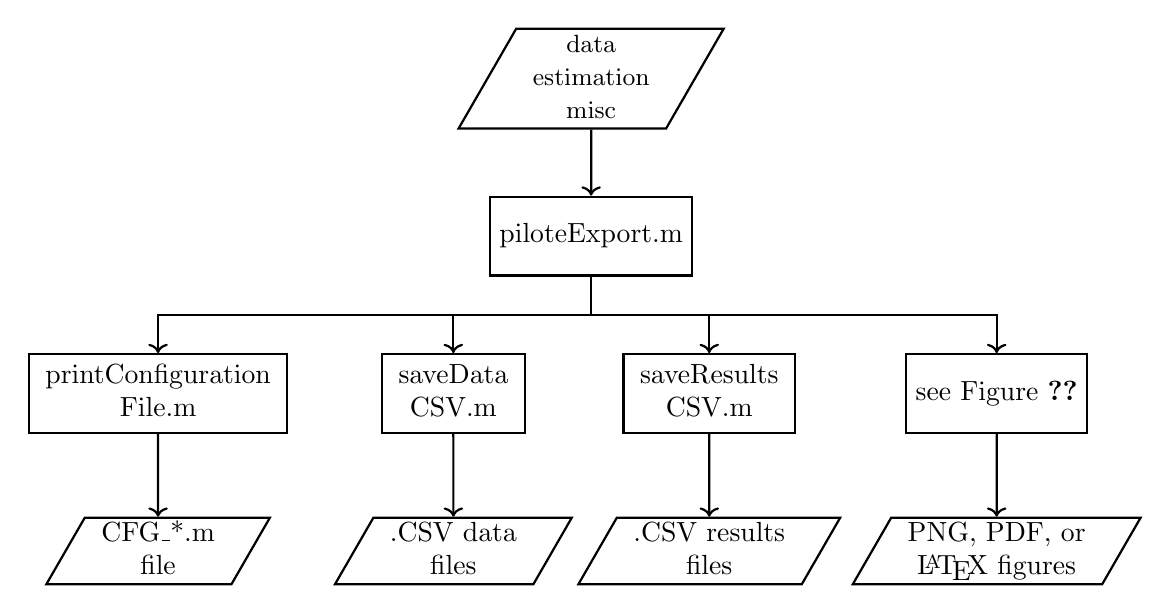
\begin{tikzpicture}

\node[parawhite](inputExport){\begin{tabular}{c} \lstinline[basicstyle = \mlttfamily \small ]!data!  \\ \lstinline[basicstyle = \mlttfamily \small ]!estimation! \\ \lstinline[basicstyle = \mlttfamily \small ]!misc!  \end{tabular}};
\node[eswhite](pilote)[below of = inputExport, yshift=-1cm, xshift = -0cm]{ \phantom{} piloteExport.m \phantom{} };
\node[eswhite](CFG)[below of = pilote, yshift=-1cm, xshift = -5.5cm]{\begin{tabular}{c} printConfiguration \\ File.m \end{tabular}};
\node[eswhite](DataCSV)[below of = pilote, yshift=-1cm, xshift = -1.75cm]{\begin{tabular}{c} saveData\\CSV.m   \end{tabular}};
\node[eswhite](ResultsCSV)[below of = pilote, yshift=-1cm, xshift = 1.5cm]{\begin{tabular}{c} saveResults\\CSV.m  \end{tabular} };
\node[eswhite](ExportFig)[below of = pilote, yshift=-1cm, xshift = 5.15cm]{ \phantom{} see Figure~\ref{FIG:ResultsVisualizationsWorkflow} \phantom{} };
\node[parawhite](outputCFG)[below of = CFG , yshift=-1cm, xshift = 0cm]{\begin{tabular}{c}  CFG\_*.m \\ file \end{tabular}};
\node[parawhite](outputDCSV)[below of = DataCSV , yshift=-1cm, xshift = 0cm]{\begin{tabular}{c} .CSV data \\ files \end{tabular}};
\node[parawhite](outputRCSV)[below of = ResultsCSV , yshift=-1cm, xshift = 0cm]{ \begin{tabular}{c} .CSV results \\ files \end{tabular}};
\node[parawhite](outputExport)[below of = ExportFig , yshift=-1cm, xshift = 0cm]{ \begin{tabular}{c} PNG, PDF, or \\ \LaTeX{} figures \end{tabular}};

\path[->, thick] (inputExport)edge(pilote);
\path[->, thick] (CFG)edge(outputCFG);
\path[->, thick] (DataCSV)edge(outputDCSV);
\path[->, thick] (ResultsCSV)edge(outputRCSV);
\path[->, thick] (ExportFig)edge(outputExport);
\path[->, draw,  thick] (pilote.south) |- (-4cm, -3cm) -| (CFG.north);
\path[->, draw,  thick] (pilote.south) |- (-2cm, -3cm) -| (DataCSV.north);
\path[->, draw,  thick] (pilote.south) |- (3cm, -3cm) -| (ResultsCSV.north);
\path[->, draw,  thick] (pilote.south) |- (5cm, -3cm) -| (ExportFig.north);

\end{tikzpicture} } 
\caption{Export options workflow} \label{FIG:ExportWorkflow}
\end{figure}







\clearpage

\input{section/OpenBDLMVersionControl}\clearpage

\section{Examples}

\section{Step-by-step example: single time-series analysis}
\label{S:ExampleDisp}

This example uses a single synthetic time series data that mimics displacement data measured on a bridge. 

\subsection{Step 1: start a project}

In the \MATLAB{} command window, type \colorbox{light-gray}{\lstinline[basicstyle = \mlttfamily \small, backgroundcolor = \color{light-gray}]!OpenBDLM_main;! }, and type $\dlsh$.
The \lstinline[basicstyle = \mlttfamily \small, backgroundcolor = \color{light-gray}]!OpenBDLM_main! starting menu appears.
The user has to provide an input from the command line each time a \lstinline[basicstyle = \mlttfamily \small, backgroundcolor = \color{light-gray}]!choice >>! appears.
The provided input is validated by typing $\dlsh$.
 \begin{lstlisting}[ frame = single, basicstyle = \mlttfamily \small, caption = {OpenBDLM command line interaction when calling \lstinline!OpenBDLM\_main();!} from \MATLAB{} command line, label = LST:OpenBDLMStartingMenuExample1 ,  float =h!, linewidth=\linewidth, captionpos=b]

------------------------------------------------
     Starting OpenBDLM_V1.0
------------------------------------------------
            Time series analysis using 
            Bayesian Dynamic Linear Models
------------------------------------------------
- Start a new project: 

     *      Enter a configuration filename 
     0   -> Interactive tool 

- Type D to Delete project(s), V for Version control, Q to Quit.

     choice >> 0
  
---------------------------------------
          Starting a new project...
----------------------------------------

- Enter a project name (max 25 characters):
     choice >> DISP
     
- Does this project aim to create synthetic data ? (y/n) 
     choice >> no

     Load data...

- Choose a database

     0   -> Build a new database     	
 
     choice >> 0
\end{lstlisting}

First, choose the interactive tool by typing \colorbox{light-gray}{\lstinline[basicstyle = \mlttfamily \small, backgroundcolor = \color{light-gray}]!0!}.
Secondly, provide a project name (e.i \lstinline[basicstyle = \mlttfamily \small, backgroundcolor = \color{light-gray}]!DISP!).
Then, answer \colorbox{light-gray}{\lstinline[basicstyle = \mlttfamily \small, backgroundcolor = \color{light-gray}]!no!} to indicate that you are not concerned with creating synthetic data.
The next step is to type \colorbox{light-gray}{\lstinline[basicstyle = \mlttfamily \small, backgroundcolor = \color{light-gray}]!0!} to indicate that you aim to load new data.

\subsection{Step 2: load the data}

At this stage, a graphical user interface \footnote{Douglas M. Schwarz, 2007, uipickfiles \url{https://www.mathworks.com/matlabcentral/fileexchange/10867-uipickfiles-uigetfile-on-steroids}} should appear on screen. 
Browse the ``data/csv'' folder to select the csv file named \lstinline[basicstyle = \mlttfamily \small, backgroundcolor = \color{light-gray}]!DISP_DISP.csv!.
Then, click on the Add button, and then the Done button, as highlighted in Figure~\ref{fig:DataLoadingUIPickFileExample1}.
You will notice that some basic information regarding the loaded time-series, such as the time series index, the reference name and the number of data points are now displayed in the \MATLAB{} command window, as depicted in Listing~\ref{LST:OpenBDLMDataAvailabilityExample1}.
At this time, three \MATLAB{} figures as those represented in Figure~\ref{fig:DataSummary1} should popup on screen.
The first figure represents the data amplitude; the second figure represents the data timestep, and the last figure the data availability.
The figures show that data points exist between August 2013 and October 2015 (see Figure~\ref{fig:DataSummary1}a).
The timestep is non-uniform; it varies from 1 hour to 25 hours (see Figure~\ref{fig:DataSummary1}b). 
The most frequent (i.e referent) time step is 1 hour.
There is no missing data (see Figure~\ref{fig:DataSummary1}c).

\begin{figure*}[h!]
\begin{center}
\includegraphics[width=0.9\linewidth]{./docfigs/Example_DISPSIM/dataloading_DISPSIM_uipickfiles_annoted.png}
\caption{Interactive data loading using the graphical user interface.}.
\label{fig:DataLoadingUIPickFileExample1}
\end{center}
\end{figure*}

 \begin{lstlisting}[ frame = single, basicstyle = \mlttfamily \small, caption = { \MATLAB{} command window output after selected data files.} from \MATLAB{} command line, label = LST:OpenBDLMDataAvailabilityExample1,  float =h!, linewidth=\linewidth, captionpos=b]
- Data available: 
 
     Time series number #      Reference name            Size                     	
     -----------------------------------------------------------------
     1                         DISP                      [19366x1]                	
     -----------------------------------------------------------------
\end{lstlisting}


\begin{figure*}[h!]
\centering
\begin{subfigure}{\linewidth}
\includegraphics[width=0.9\linewidth]{./docfigs/Example_DISPSIM/raw/ALL_AMPLITUDES.pdf}
\caption{Amplitude}
\end{subfigure}
\begin{subfigure}{\linewidth}
\includegraphics[width=0.9\linewidth]{./docfigs/Example_DISPSIM/raw/ALL_TIMESTEPS.pdf} 
\caption{Timestep}
\end{subfigure}
\begin{subfigure}{\linewidth}
\includegraphics[width=0.9\linewidth]{./docfigs/Example_DISPSIM/raw/AVAILABILITY.pdf}
\caption{Availbility}
\end{subfigure}
\caption{Data used in Section~\ref{S:ExampleDisp}}.
\label{fig:DataSummary1}
\end{figure*}

\subsection{Step 3: edit and pre-process the data}

The next step of the analysis consists in editing or preprocessing the data.
The data editing and preprocessing menu as depicted in Listing~\ref{LST:Editing_menu} appear.
In this example, the objective is to use the data as such, so no editing or preprocessing is done.
Therefore, type \colorbox{light-gray}{\lstinline[basicstyle = \mlttfamily \small, backgroundcolor = \color{light-gray}]!7!} to save the data as such, and continue analysis.

\subsection{Step 4: configure the model}

The next step is to configure the model.
First, the program requests the number of model class.
In this exemple, the time series data looks stationary and we are not interested in anomaly detection, so type type \colorbox{light-gray}{\lstinline[basicstyle = \mlttfamily \small, backgroundcolor = \color{light-gray}]!1!}.
Secondly, OpenBDLM asks for the type of block component. 
Type \colorbox{light-gray}{\lstinline[basicstyle = \mlttfamily \small, backgroundcolor = \color{light-gray}]![11 31 31 41]!} to define a model with a local level, a yearly periodic component, a daily periodic component and an autoregressive component.
The  output on \MATLAB{} command window during interactive model configuration is presented in Listing~\ref{LST:OpenBDLMModelConfigureExample1}.
Type $\dlsh$ to valid.
The model is then built, a {\lstinline[basicstyle = \mlttfamily \small, backgroundcolor = \color{light-gray}]!DATA_DISP.mat!} binary data file, a {\lstinline[basicstyle = \mlttfamily \small, backgroundcolor = \color{light-gray}]!CFG_DISP.m!} configuration file, as well as a {\lstinline[basicstyle = \mlttfamily \small, backgroundcolor = \color{light-gray}]!PROJ_DISP.mat!} project file are created.
The OpenBLDM main menu must appear on the \MATLAB{} command window (see Listing~\ref{LST:OpenBDLMMainMenu}).
Type \colorbox{light-gray}{\lstinline[basicstyle = \mlttfamily \small, backgroundcolor = \color{light-gray}]!Q!} to save and quit.

 \begin{lstlisting}[ frame = single, basicstyle = \mlttfamily \small, caption = { \MATLAB{} command window output during interactive model configuration.}, label = LST:OpenBDLMModelConfigureExample1,  float =h, linewidth=\linewidth, captionpos=b]
- How many model classes do you want for each time-series? 
     choice >> 1
     
     --------------------------------------------------------
     BDLM Component reference numbers
     --------------------------------------------------------
     11: Local level 
     12: Local trend 
     13: Local acceleration 
     21: Local level compatible with local trend 
     22: Local level compatible with local acceleration 
     23: Local trend compatible with local acceleration 
     31: Periodic 
     41: Autoregressive process (AR(1)) 
     51: Kernel regression 
     61: Level Intervention 
     --------------------------------------------------------

- Identify components for time series #1; e.g. [11 31 41]
     choice >> [11 31 31 41]

     Building model...
     Saving project...
     Project saved in saved_projects/PROJ_DISP.mat. 
     Printing configuration file...
     Saving data...

     Database saved in data/mat/DATA_DISP.mat 
     Configuration file saved in config_files/CFG_DISP.m. 

\end{lstlisting}


\subsection{Step 5: open the configuration file}

After the data loading and the model configuration, a configuration file named \lstinline[basicstyle = \mlttfamily \small, backgroundcolor = \color{light-gray}]!CFG_DISP.csv! is automatically created and saved in ``config\_files'' folder.
Open the configuration file from \MATLAB{} command line by typing  \colorbox{light-gray}{\lstinline[basicstyle = \mlttfamily \small, backgroundcolor = \color{light-gray}]!edit CFG_DISP.m!}.
The first part of this configuration file as it should appear on the \MATLAB{} editor is shown in Listing~\ref{LST:CFGFileExample1}.
The Model parameters section of the configuration file shows that the model totalizes 8 model parameters, that is 
\begin{gather*}
\bm\theta=\{\sigma_{w}^{LL}, p^{\text{PD1}}, \sigma_{w}^{\text{PD1}} , p^{\text{PD2}}, \sigma_{w}^{\text{PD2}}, \phi^{AR}, \sigma_{w}^{AR}, \sigma_{v}\}.
\end{gather*}
%The default value of the model parameters are assigned   using heuristic knowledge or computed from the data using statistics on the data.
The default model parameters values are 
\begin{gather*}
\bm\theta^{\text{default}}=\{0, 365.2422, 0, 1, 0, 0.75, 0.0174, 0.0087002 \}.
\end{gather*}
%In the same manner, default value for the initial hidden states are assigned using heuristic knowledge or computed using statistics on the data.
The default  hidden states mean  and covariance values are 
\begin{align*}
\bm \mu^{\text{default}}_{0} & = [25.8 , 5  ,   	0     ,	5   ,  	0    , 	0     ]^{\intercal}, \text{and} \\
 \text{diag}(\bm\Sigma^{\text{default}}_{0}) & = [	0.121 	,0.121 ,	0.121 ,	0.121 ,	0.121 	, 0.0303     ], 
 \end{align*}
 respectively.

%\subsection{Step 6: results using defaults model parameters and default initial hidden states}

%Note that, by default, OpenBDLM considers that the parameters $\sigma_{w}^{LL}$, $P1$, $\sigma_{w}^{P1}$ , $P2$, $\sigma_{w}^{P2}$ are known.


% \lstinline[basicstyle = \mlttfamily \small ]!model.param_properties! 

\begin{lstlisting}[linewidth=\linewidth, style=Matlab-editor,  basicstyle = \mlttfamily \scriptsize, backgroundcolor = \color{matlab-yellow}, caption = {Example of a configuration file}, label=LST:CFGFileExample1, ,captionpos=b, float=h!]
%                    OpenBDLM configuration file                          
%          Autogenerated by OpenBDLM on 22-Nov-2018 17:18:09              
%
%% A - Project name
misc.ProjectName='DISP';

%% B - Data
dat=load('DATA_DISP.mat'); 
data.values=dat.values;
data.timestamps=dat.timestamps;
data.labels={'DISP'};

%% C - Model structure 
% Components reference numbers
% 11: Local level
% 12: Local trend
% 13: Local acceleration
% 21: Local level compatible with local trend
% 22: Local level compatible with local acceleration
% 23: Local trend compatible with local acceleration
% 31: Periodic
% 41: Autoregressive
% 51: Kernel regression
% 61: Level Intervention

% Model components
% Model 1
model.components.block{1}={[11 31 31 41] };

% Model component constrains | Take the same  parameter as model class #1
 
% Model inter-components dependence | {[components form dataset_i depends on components from  dataset_j]_i,[...]}
model.components.ic={[ ] };
%
%% D - Model parameters 
model.param_properties={
     % #1       #2       #3    #4    #5         #6       #7     #8     #9    #10
     % Param name Block name  Model Obs Bound Prior Mean Std Values Ref
     '\sigma_w', 'LL',  '1',   '1', [NaN  NaN],    'N/A',  NaN, NaN,  0,          1 %#1   
     'p',        'PD1', '1',   '1', [NaN  NaN],    'N/A',  NaN, NaN, 365.24,      2 %#2   
     '\sigma_w', 'PD1', '1',   '1', [NaN  NaN],    'N/A',  NaN, NaN,   0,         3 %#3   
     'p',        'PD2', '1',   '1', [NaN  NaN],    'N/A',  NaN, NaN,   1,         4 %#4   
     '\sigma_w', 'PD2', '1',   '1', [NaN  NaN],    'N/A',  NaN, NaN,   0,         5 %#5   
     '\phi',     'AR',  '1',   '1', [0  1],        'N/A',  NaN, NaN,   0.75,      6 %#6   
     '\sigma_w', 'AR',  '1',   '1', [0  Inf],      'N/A',  NaN, NaN,   0.0174,    7 %#7   
     '\sigma_v', '',    '1',   '1', [0  Inf],      'N/A',  NaN, NaN,   0.0087002, 8 %#8   
};

%% E - Initial states values 
% Initial hidden states mean for model 1:
model.initX{ 1 }=[	25.8  	5     	0     	5     	0     	0     ]';

% Initial hidden states variance for model 1: 
model.initV{ 1 }=diag([ 	0.121 	0.121 	0.121 	0.121 	0.121 	0.0303 ]);

% Initial probability for model 1
model.initS{1}=[1     ];

\end{lstlisting}

\subsection{Step 6: estimate the hidden states}

Type \colorbox{light-gray}{\lstinline[basicstyle = \mlttfamily \small, backgroundcolor = \color{light-gray}]!OpenBDLM_main('CFG_DISP.m');!} in the \MATLAB{} command line.
Once, the main menu appears, type  \colorbox{light-gray}{\lstinline[basicstyle = \mlttfamily \small, backgroundcolor = \color{light-gray}]!3!}, then \colorbox{light-gray}{\lstinline[basicstyle = \mlttfamily \small, backgroundcolor = \color{light-gray}]!1!} to estimate the filtered hidden states using the default model parameters and default initial hidden states values.
The value of the log-likelihood is $38627$, and the estimated hidden states are presented in Figure~\ref{fig:DISPSIMDefaultDefaultExample1}.

\begin{figure*}[h!]
\centering
\begin{subfigure}{\linewidth}
\includegraphics[width=0.9\linewidth]{./docfigs/Example_DISPSIM/default/DISP_ObservedPredicted.pdf} 
\caption{Observed and estimated displacement data}
\end{subfigure}
\begin{subfigure}{\linewidth}
\includegraphics[width=0.9\linewidth]{./docfigs/Example_DISPSIM/default/DISP_LL_1.pdf}
\caption{Estimated displacement local level component}.
\end{subfigure}
\begin{subfigure}{\linewidth}
\includegraphics[width=0.9\linewidth]{./docfigs/Example_DISPSIM/default/DISP_S1_2.pdf}
\caption{Estimated displacement yearly periodic component}
\end{subfigure}
\begin{subfigure}{\linewidth}
\includegraphics[width=0.9\linewidth]{./docfigs/Example_DISPSIM/default/DISP_S1_4.pdf}
\caption{Estimated displacement daily periodic component}
\end{subfigure}
\begin{subfigure}{\linewidth}
\includegraphics[width=0.9\linewidth]{./docfigs/Example_DISPSIM/default/DISP_AR_6.pdf} 
\caption{Estimated displacement autoregressive component}
\end{subfigure}
\caption{Estimated results using OpenBDLM defaults model parameters and default initial hidden states. The hidden states are estimated from the data presented in Figure~\ref{fig:DataSummary1}a. The solid line and shaded area represent the mean and standard deviation of the estimated hidden states, respectively.}
\label{fig:DISPSIMDefaultDefaultExample1}
\end{figure*}

\subsection{Step 7: estimate the model parameters from the data}

Type \colorbox{light-gray}{\lstinline[basicstyle = \mlttfamily \small, backgroundcolor = \color{light-gray}]!OpenBDLM_main('CFG_DISP.m');!} in the \MATLAB{} command line.
Once, the main menu appears, type  \colorbox{light-gray}{\lstinline[basicstyle = \mlttfamily \small, backgroundcolor = \color{light-gray}]!1!}, then \colorbox{light-gray}{\lstinline[basicstyle = \mlttfamily \small, backgroundcolor = \color{light-gray}]!1!} to estimate the model parameters using Newton-Raphson (type  \colorbox{light-gray}{\lstinline[basicstyle = \mlttfamily \small, backgroundcolor = \color{light-gray}]!1!} to use the Stochastic Gradient instead).
The model parameters learning procedure starts, and messages are printed on \MATLAB{} command window to monitor the convergence through iterations (see Listing~\ref{LST:OpenBLDMModelParameterLearning}).
Note that, by default, OpenBDLM considers that the parameters $\sigma_{w}^{LL}$, $PD1$, $\sigma_{w}^{PD1}$ , $PD2$, $\sigma_{w}^{PD2}$ are known.
Therefore, there are three model parameters to be learned from the data in this example.
The estimation of the model parameters may take several hours.
Once the algorithm converged, the optimized model parameters values should be close to \footnote{Note that it is possible to get slightly different value of parameters with the same performance.}
\begin{gather*}
\bm\theta^{\text{*}}=\{0, 365.2422, 0, 1, 0, 0.97, 0.0192, 7.4258\times10^{-7} \}.
\end{gather*}

\subsection{Step 8: estimate the hidden states using the optimized model parameters values}

Type \colorbox{light-gray}{\lstinline[basicstyle = \mlttfamily \small, backgroundcolor = \color{light-gray}]!OpenBDLM_main('CFG_DISP_optim.m');!} in the \MATLAB{} command line to load the configuration file  \lstinline[basicstyle = \mlttfamily \small, backgroundcolor = \color{light-gray}]!CFG_DISP_optim.m'!.
 \lstinline[basicstyle = \mlttfamily \small, backgroundcolor = \color{light-gray}]!CFG_DISP_optim.m'! contains optimized model parameters previously estimated using the Newton-Raphson algorithm.
Once the main menu appears, type  \colorbox{light-gray}{\lstinline[basicstyle = \mlttfamily \small, backgroundcolor = \color{light-gray}]!3!}, then \colorbox{light-gray}{\lstinline[basicstyle = \mlttfamily \small, backgroundcolor = \color{light-gray}]!1!} to estimate the filtered hidden states using the optimized model parameters and default initial hidden states values.
The value of the log-likelihood is now $48819$.
The estimated hidden states are presented in Figure~\ref{fig:DISPSIMOptimizedDefaultExample1}.

\begin{figure*}[h!]
\begin{center}
\begin{subfigure}{\linewidth}
\includegraphics[width=0.9\linewidth]{./docfigs/Example_DISPSIM/optim_param_default_initialhiddenstate/DISP_ObservedPredicted.pdf}
\caption{Observed and estimated displacement data}
\end{subfigure}
\begin{subfigure}{\linewidth}
\includegraphics[width=0.9\linewidth]{./docfigs/Example_DISPSIM/optim_param_default_initialhiddenstate/DISP_LL_1.pdf}
\caption{Estimated displacement local level.}
\end{subfigure}
\begin{subfigure}{\linewidth}
\includegraphics[width=0.9\linewidth]{./docfigs/Example_DISPSIM/optim_param_default_initialhiddenstate/DISP_S1_2.pdf}
\caption{Estimated displacement yearly periodic component (first hidden state)}
\end{subfigure}
\begin{subfigure}{\linewidth}
\includegraphics[width=0.9\linewidth]{./docfigs/Example_DISPSIM/optim_param_default_initialhiddenstate/DISP_S1_4.pdf} 
\caption{Estimated displacement daily periodic component (first hidden state)}
\end{subfigure}
\begin{subfigure}{\linewidth}
\includegraphics[width=0.9\linewidth]{./docfigs/Example_DISPSIM/optim_param_default_initialhiddenstate/DISP_AR_6.pdf} 
\caption{Estimated displacement autoregressive component}
\end{subfigure}
\caption{Estimated results using OpenBDLM optimized model parameters and default initial hidden states. The hidden states are estimated from the data presented in Figure~\ref{fig:DataSummary1}a. The solid line and shaded area represent the mean and standard deviation of the estimated hidden states, respectively.}
\label{fig:DISPSIMOptimizedDefaultExample1}
\end{center}
\end{figure*}

\subsection{Step 9: estimate the initial hidden states}

Type \colorbox{light-gray}{\lstinline[basicstyle = \mlttfamily \small, backgroundcolor = \color{light-gray}]!OpenBDLM_main('CFG_DISP_optim.m');!} in the \MATLAB{} command line.
Then, type  \colorbox{light-gray}{\lstinline[basicstyle = \mlttfamily \small, backgroundcolor = \color{light-gray}]!2!}, to optimize the initial hidden states value.
The estimated initial hidden states mean and covariance values are 
\begin{align*}
\bm \mu^{*}_{0} & = [	25.9  ,	-0.204,	-0.00288 ,	0.0341,	0.0521	, -0.0436  ]^{\intercal}, \text{and} \\
 \text{diag}(\bm\Sigma^{*}_{0}) & = [	3.74\times10^{-5} ,	6.87\times10^{-5}	, 7\times10^{-5} ,	5.73\times10^{-7} ,	5.73\times10^{-7} ,	0.000493    ], 
 \end{align*}
 respectively.
Once it is done, type  \colorbox{light-gray}{\lstinline[basicstyle = \mlttfamily \small, backgroundcolor = \color{light-gray}]!2!}, and then  \colorbox{light-gray}{\lstinline[basicstyle = \mlttfamily \small, backgroundcolor = \color{light-gray}]!1!} to compute the filtered hidden states using the optimized model parameters and optimized initial hidden states.
The value of the log-likelihood is $49056$.
The estimated hidden states are presented in Figure~\ref{fig:DISPSIMOptimizedOptimizedExample1}.


\begin{figure*}[h!]
\begin{center}
\begin{subfigure}{\linewidth}
\includegraphics[width=0.9\linewidth]{./docfigs/Example_DISPSIM/optim_param_optim_initialhiddenstate/DISP_ObservedPredicted.pdf} 
\caption{Observed and estimated displacement data}
\end{subfigure}
\begin{subfigure}{\linewidth}
\includegraphics[width=0.9\linewidth]{./docfigs/Example_DISPSIM/optim_param_optim_initialhiddenstate/DISP_LL_1.pdf}
\caption{Estimated displacement local level component.}
\end{subfigure}
\begin{subfigure}{\linewidth}
\includegraphics[width=0.9\linewidth]{./docfigs/Example_DISPSIM/optim_param_optim_initialhiddenstate/DISP_S1_2.pdf} 
\caption{Estimated displacement yearly periodic component (first hidden state)}
\end{subfigure}
\begin{subfigure}{\linewidth}
\includegraphics[width=0.9\linewidth]{./docfigs/Example_DISPSIM/optim_param_optim_initialhiddenstate/DISP_S1_4.pdf}
\caption{Estimated displacement daily periodic component (first hidden state)}
\end{subfigure}
\begin{subfigure}{\linewidth}
\includegraphics[width=0.9\linewidth]{./docfigs/Example_DISPSIM/optim_param_optim_initialhiddenstate/DISP_AR_6.pdf} 
\caption{Estimated displacement autoregressive component}
\end{subfigure}
\caption{Estimated results using OpenBDLM optimized model parameters and optimized initial hidden states. The hidden states are estimated from the data presented in Figure~\ref{fig:DataSummary1}a. The solid line and shaded area represent the mean and standard deviation of the estimated hidden states, respectively.}
\label{fig:DISPSIMOptimizedOptimizedExample1}
\end{center}
\end{figure*}\clearpage

\subsection{Example \#2: dependence model between two time series}
\label{S:ExampleDispTemp}

\subsubsection{Data description}

This example uses two synthetic time series that mimics the displacement and temperature data measured on a bridge.
The  Figure~\ref{fig:DataSummaryRaw2}a shows that data points exist between August 2013 and October 2015.
The timestep in the original data is non-uniform; it varies from 1 hour to 25 hours (see Figure~\ref{fig:DataSummaryRaw2}b). 
The timestep vector is not identical on each time series. 
It means that the time series are not synchronized between each other.
The most frequent (i.e referent) time step is 1 hour for both time series (Section~\ref{SS:NonUniform}).
There is no missing data (\lstinline[basicstyle = \mlttfamily \small, backgroundcolor = \color{light-gray}]!NaN!) on the displacement time series, but there are missing data on the temperature time series as indicated by the red crosses on the Figure~\ref{fig:DataSummaryRaw2}c.
Each red cross indicates the presence of a Not a Number (\lstinline[basicstyle = \mlttfamily \small, backgroundcolor = \color{light-gray}]!NaN!) value in the time series.
After data synchronization, the time step vectors are identical on each time series (Figure~\ref{fig:DataSummaryDefaultPreProcessed2}).
Both time series are stationary, and they exhibit a level, a yearly and daily periodic pattern as well as an autoregressive pattern.
The periodic patterns observed on the displacement time series is due to the temperature variations observed in the temperature time series.

In this example, we choose to resample the original data in order to have timesteps of 6h instead of 1h. 

\begin{figure*}[h!]
\centering
\begin{subfigure}{\linewidth}
\centering
\includegraphics[width=0.9\linewidth]{./docfigs/Example_DISPTEMPSIM/raw/ALL_AMPLITUDES.pdf} 
\caption{Amplitude}
\end{subfigure}
\begin{subfigure}{\linewidth}
\centering
\includegraphics[width=0.9\linewidth]{./docfigs/Example_DISPTEMPSIM/raw/ALL_TIMESTEPS.pdf}
\caption{Timestep}
\end{subfigure}
\begin{subfigure}{\linewidth}
\centering
\includegraphics[width=0.9\linewidth]{./docfigs/Example_DISPTEMPSIM/raw/AVAILABILITY.pdf}
\caption{Availability}
\end{subfigure}
\caption{Raw data in the example \#2 where the reference timestep is 1h.}
\label{fig:DataSummaryRaw2}
\end{figure*}


\begin{figure*}[h!]
\centering
\begin{subfigure}{\linewidth}
\centering
\includegraphics[width=0.9\linewidth]{./docfigs/Example_DISPTEMPSIM/preprocessed_default/ALL_AMPLITUDES.pdf} 
\caption{Amplitude}
\end{subfigure}
\begin{subfigure}{\linewidth}
\centering
\includegraphics[width=0.9\linewidth]{./docfigs/Example_DISPTEMPSIM/preprocessed_default/ALL_TIMESTEPS.pdf}
\caption{Timestep}
\end{subfigure}
\begin{subfigure}{\linewidth}
\centering
\includegraphics[width=0.9\linewidth]{./docfigs/Example_DISPTEMPSIM/preprocessed_default/AVAILABILITY.pdf}
\caption{Availability}
\end{subfigure}
\caption{Data used in example \#2 after resampling to obtain a reference timestep of 6h.}
\label{fig:DataSummaryDefaultPreProcessed2}
\end{figure*}



\subsubsection{Model description}
\label{SS:ModelConstructionExample2}

The model includes one model class, and the hidden state variables are 
\begin{gather*}
\textbf{x}=[x^{\mathtt{LL}}_{\mathtt{D}}, x^{\mathtt{AR}}_{\mathtt{D}}, x^{\mathtt{LL}}_{\mathtt{T}}, x^{\mathtt{P1}\text{,yearly}}_{\mathtt{T}}, x^{\mathtt{P2}\text{,yearly}}_{\mathtt{T}}, x^{\mathtt{P1}\text{,daily}}_{\mathtt{T}} , x^{\mathtt{P2}\text{,daily}}_{T}, x^{\mathtt{AR}}_{\mathtt{T}}],
\end{gather*}
where $\mathtt{D}$ and $\mathtt{T}$ refer to the displacement and temperature time series, respectively.
The periodic patterns observed on the displacement are considered through a dependency of the displacement on the hidden state variables of the periodic  and autoregressive components of the temperature time series (Section~\ref{S:Dependencies}).
The associated model parameters are
\begin{align*}
\bm\theta & =[\sigma_{w, \mathtt{D}}^{\mathtt{LL}}, \phi^{\mathtt{AR}}_{D}, \sigma_{w, \mathtt{D}}^{\mathtt{AR}}, \sigma_{v, \mathtt{D}},  \\
&  \sigma_{w, \mathtt{T}}^{\mathtt{LL}},  p^{\mathtt{P}, \text{yearly}}_{\mathtt{T}}, \sigma_{w, \mathtt{T}}^{\mathtt{P}, \text{yearly}} , p^{\mathtt{P}, \text{daily}}_{\mathtt{T}} , \sigma_{w, \mathtt{T}}^{\mathtt{P}, \text{daily}}, \phi^{\mathtt{AR}}_{\mathtt{T}}, \sigma_{w, \mathtt{T}}^{\mathtt{AR}}, \sigma_{v, \mathtt{T}},\phi^{\mathtt{D}|\mathtt{T}}_{\mathtt{P}_{y}},\phi^{\mathtt{D}|\mathtt{T}}_{\mathtt{P}_{d}},\phi^{\mathtt{D}|\mathtt{T}}_{\mathtt{AR}}].
\end{align*}
The optimized model parameters values computed using the Newton-Raphson algorithm (see~\ref{SS:THModelParameterEstimation}) with a training period of 180 days are
\begin{align*}
 \bm\theta^{\text{*}}& =[0, 0.90, 0.037, 1.94\times10^{-5},  \\
 & 0, 365.2422, 0, 1, 0, 0.98, 0.86, 1.14\times10^{-4}, -0.013, 0.0706, 0.00073 ].
\end{align*}
The estimated initial hidden states mean and covariance values are 
\begin{align*}
\bm \mu^{*}_{0} & = [	25.9,-2.55\times10^{-5},5.53,16.3,-0.999,0.263,0.669,3.77 ]^{\intercal}, \text{and} \\
\bm\Sigma^{*}_{0} & = \text{diag}([4.27\times10^{-5},1.68\times10^{-3},0.715,0.338,0.341,6.73\times10^{-5},6.73\times10^{-5},1.81]).
 \end{align*}
The hidden states computed using the estimated model parameters and initial hidden states are presented in Figure~\ref{fig:DISPTEMPSIMOptimizedOptimizedExample2}.


\subsubsection{Run the example from the pre-existing configuration file}
\label{SS:LoadConfigFileEx2}
There is a configuration file CFG\_Example\_DISPTEMP\_optim.m which is located in the ``config\_files'' folder of the OpenBDLM package.
CFG\_Example\_DISPTEMP\_optim.m contains the optimized model parameters and optimized initial hidden states values.
There is also a data file DATA\_Example\_DISPTEMP\_optim.mat that is located in the ``data/mat'' subfolder.
Therefore, it is possible to run the example \#2 by following the steps below while interacting with the \MATLAB{} command line:
\begin{enumerate}
\item Start OpenBDLM. Type \colorbox{light-gray}{\lstinline[basicstyle = \mlttfamily \small, backgroundcolor = \color{light-gray}]!OpenBDLM_main('CFG_Example_DISPTEMP_optim.m');!}.
\item Access hidden states estimation menu. Type \colorbox{light-gray}{\lstinline[basicstyle = \mlttfamily \small, backgroundcolor = \color{light-gray}]!3!}.
\item Run the Kalman filter to estimate the hidden states. Type \colorbox{light-gray}{\lstinline[basicstyle = \mlttfamily \small, backgroundcolor = \color{light-gray}]!1!}.
\item Save and quit. Type \colorbox{light-gray}{\lstinline[basicstyle = \mlttfamily \small, backgroundcolor = \color{light-gray}]!Q!}.
\end{enumerate}


\subsubsection{Run the example from command line interaction}

The analysis of a new dataset usually requires to start from scratch.
This section explains how to run the example \#2 from scratch, that is, how to load  and resample the data presented in Figure~\ref{fig:DataSummaryRaw2}, configure the model, estimate the model parameters and estimate the hidden states.
This may be done by following steps below while interacting with the \MATLAB{} command line:
\begin{enumerate}
\item Start OpenBDLM. Type \colorbox{light-gray}{\lstinline[basicstyle = \mlttfamily \small, backgroundcolor = \color{light-gray}]!OpenBDLM_main;!}.
\item Choose the interactive tool. Type \colorbox{light-gray}{\lstinline[basicstyle = \mlttfamily \small, backgroundcolor = \color{light-gray}]!0!}.
\item Enter the project name. Type \colorbox{light-gray}{\lstinline[basicstyle = \mlttfamily \small, backgroundcolor = \color{light-gray}]!Example_DISPTEMP!}. 
\item Disregard generating synthetic data. Type \colorbox{light-gray}{\lstinline[basicstyle = \mlttfamily \small, backgroundcolor = \color{light-gray}]!no!}. 
\item Load new data. Type \colorbox{light-gray}{\lstinline[basicstyle = \mlttfamily \small, backgroundcolor = \color{light-gray}]!0!}.
\item Select from the graphical user interface the data files located in the ``/data/csv/Example\_DISPTEMP/'' folder. The Figure~\ref{fig:DataSummaryRaw2} that represents the raw data should popup on screen.
\item Access the resampling menu. Type \colorbox{light-gray}{\lstinline[basicstyle = \mlttfamily \small, backgroundcolor = \color{light-gray}]!4!}. 

\item Resample data to obtain timesteps of 6h (0.25 day). Type \colorbox{light-gray}{\lstinline[basicstyle = \mlttfamily \small, backgroundcolor = \color{light-gray}]!0.25!}. The Figure \ref{fig:DataSummaryDefaultPreProcessed2} should popup on the screen this time for the resampled data.

\item Save and continue. Type \colorbox{light-gray}{\lstinline[basicstyle = \mlttfamily \small, backgroundcolor = \color{light-gray}]!7!}. The same figures should popup on the screen again.
\item Select dependency for the time series \#1. Type \colorbox{light-gray}{\lstinline[basicstyle = \mlttfamily \small, backgroundcolor = \color{light-gray}]![2]!}.
\item Select dependency for the time series \#2. Type \colorbox{light-gray}{\lstinline[basicstyle = \mlttfamily \small, backgroundcolor = \color{light-gray}]![0]!}.
\item Select the number of model classes. Type \colorbox{light-gray}{\lstinline[basicstyle = \mlttfamily \small, backgroundcolor = \color{light-gray}]!1!}. 
\item Select the model block components for time series \#1. Type \colorbox{light-gray}{\lstinline[basicstyle = \mlttfamily \small, backgroundcolor = \color{light-gray}]![11 41]!}.
\item Select the model block components for time series \#2. Type \colorbox{light-gray}{\lstinline[basicstyle = \mlttfamily \small, backgroundcolor = \color{light-gray}]![11 31 31 41]!}.

\item Access the training period modification menu. Type \colorbox{light-gray}{\lstinline[basicstyle = \mlttfamily \small, backgroundcolor = \color{light-gray}]!13!}. 

\item Modify the training period. Type \colorbox{light-gray}{\lstinline[basicstyle = \mlttfamily \small, backgroundcolor = \color{light-gray}]!1!}. 

\item Choose the starting time (day). Type \colorbox{light-gray}{\lstinline[basicstyle = \mlttfamily \small, backgroundcolor = \color{light-gray}]!1!}. 

\item Choose the end time (day). Type \colorbox{light-gray}{\lstinline[basicstyle = \mlttfamily \small, backgroundcolor = \color{light-gray}]!180!}. 

%\item Access hidden states estimation menu. Type \colorbox{light-gray}{\lstinline[basicstyle = \mlttfamily \small, backgroundcolor = \color{light-gray}]!3!}. 
%\item Change the state estimation method to UD\footnote{The UD computation is required in this case because of the presence of missing data. See Section~\ref{SS:KFUD} for more details.}. Type \colorbox{light-gray}{\lstinline[basicstyle = \mlttfamily \small, backgroundcolor = \color{light-gray}]!3!}. 
%\item Return to the main menu. Type \colorbox{light-gray}{\lstinline[basicstyle = \mlttfamily \small, backgroundcolor = \color{light-gray}]!R!}.
\item Access model parameter estimation menu. Type \colorbox{light-gray}{\lstinline[basicstyle = \mlttfamily \small, backgroundcolor = \color{light-gray}]!1!}. 
\item Start the Newton-Raphson algorithm. Type \colorbox{light-gray}{\lstinline[basicstyle = \mlttfamily \small, backgroundcolor = \color{light-gray}]!1!}. Once the algorithm has converged, the optimized model parameters values should be close to the values presented in \S\ref{SS:ModelConstructionExample2}. Note also that it is possible to get slightly different parameter values\footnote{Keep in mind that the optimization may take several minutes. It is possible to abort the analysis here and to load the configuration file called CFG\_Example\_DISPTEMP\_optim.m to load pre-computed values of model parameters, as presented in Section~\ref{SS:LoadConfigFileEx2}.}.
\item Estimate the initial hidden states values. Type \colorbox{light-gray}{\lstinline[basicstyle = \mlttfamily \small, backgroundcolor = \color{light-gray}]!2!}.
\item Estimate the hidden states using the Kalman filter. Type \colorbox{light-gray}{\lstinline[basicstyle = \mlttfamily \small, backgroundcolor = \color{light-gray}]!1!}. The estimation should be similar to the results presented in Figure~\ref{fig:DISPTEMPSIMOptimizedOptimizedExample2}.
\item Access export menu. Type \colorbox{light-gray}{\lstinline[basicstyle = \mlttfamily \small, backgroundcolor = \color{light-gray}]!17!}. 
\item Export the current project in a configuration file. Type \colorbox{light-gray}{\lstinline[basicstyle = \mlttfamily \small, backgroundcolor = \color{light-gray}]!1!}.
\item Save and quit OpenBDLM. Type \colorbox{light-gray}{\lstinline[basicstyle = \mlttfamily \small, backgroundcolor = \color{light-gray}]!Q!}.
\end{enumerate}




%\subsection{Step 4: configure the model}
%
%The next step is to configure the model.
%First, the program requests the number of model class.
%In this exemple, the time series data looks stationary and we are not interested in anomaly detection, and therefore we type \colorbox{light-gray}{\lstinline[basicstyle = \mlttfamily \small, backgroundcolor = \color{light-gray}]!1!}.
%Secondly, because there are several time series, OpenBDLM needs to know if there are dependencies between the time series.
%Typing \colorbox{light-gray}{\lstinline[basicstyle = \mlttfamily \small, backgroundcolor = \color{light-gray}]!2!} for the first time series, and \colorbox{light-gray}{\lstinline[basicstyle = \mlttfamily \small, backgroundcolor = \color{light-gray}]!0!} for the second time series means that the model will consider the irreversible components (if any) of the second (temperature) time series as covariates to describe the irreversible patterns observed in the first (displacement) time series.
%Then, OpenBDLM asks for the type of block component for each time series. 
%Type \colorbox{light-gray}{\lstinline[basicstyle = \mlttfamily \small, backgroundcolor = \color{light-gray}]![11 41]!} for the displacement time series and \colorbox{light-gray}{\lstinline[basicstyle = \mlttfamily \small, backgroundcolor = \color{light-gray}]![11 31 31 41]!} for the temperature time series.
%The yearly and daily periodic patterns observed in the displacement time series are modelled using the dependence on the periodic components defined for modelling the temperature time series data.
%Note that because an autoregressive component is chosen for the displacement time series data, the time-dependent model error on the displacement is modelled using a dependence on the autoregressive component of the temperature time series data, as well as an independent autoregressive component.
%The  output on \MATLAB{} command window during interactive model configuration is presented in Listing~\ref{LST:OpenBDLMModelConfigureExample2}.
%Type $\dlsh$ to valid.
%The model is then built, a \lstinline[basicstyle = \mlttfamily \small, backgroundcolor = \color{light-gray}]!DATA_DISPTEMP.mat! binary data file, a \lstinline[basicstyle = \mlttfamily \small, backgroundcolor = \color{light-gray}]!CFG_DISPTEMP.m! configuration file, as well as a \lstinline[basicstyle = \mlttfamily \small, backgroundcolor = \color{light-gray}]!PROJ_DISPTEMP.mat! project file are created.
%The OpenBLDM main menu must appear on the \MATLAB{} command window (see Listing~\ref{LST:OpenBDLMMainMenu}).
%Type \colorbox{light-gray}{\lstinline[basicstyle = \mlttfamily \small, backgroundcolor = \color{light-gray}]!Q!} to save and quit.



% \begin{lstlisting}[ frame = single, basicstyle = \mlttfamily \small, caption = { \MATLAB{} command window output during model configuration}, label = LST:OpenBDLMModelConfigureExample2,  float =h!, linewidth=\linewidth, captionpos=b, breaklines=true]
%- Identifies dependence between time series; use [0] to indicate no dependence
%    time serie #1 depends on time series # >> [2]
%
%- Identifies dependence between time series; use [0] to indicate no dependence
%    time serie #2 depends on time series # >> [0]
%
%- How many model classes do you want for each time series? 
%     choice >> 1
%     
%     ------------------------------------
%          BDLM Component reference numbers
%     ------------------------------------
%     11: Local level 
%     12: Local trend 
%     13: Local acceleration 
%     21: Local level compatible with local trend 
%     22: Local level compatible with local acceleration 
%     23: Local trend compatible with local acceleration 
%     31: Periodic 
%     41: Autoregressive process (AR(1)) 
%     51: Kernel regression 
%     61: Level Intervention 
%     --------------------------------------
%
%- Identify components for time series #1; e.g. [11 31 41]
%     choice >> [11 41]
%
%- Identify components for time series #2; e.g. [11 31 41]
%     choice >> [11 31 31 41]
%
%     Building model...
%     Saving project...
%     Project saved in saved_projects/PROJ_Example_DISPTEMP.mat. 
%     Printing configuration file...
%     Saving data...
%     Database saved in data/mat/DATA_Example_DISPTEMP.mat 
%     Configuration file saved in config_files/CFG_Example_DISPTEMP.m. 
%\end{lstlisting}


%\subsection{Step 5: open the configuration file}
%
%After the data loading and the model configuration, a configuration file named \lstinline[basicstyle = \mlttfamily \small, backgroundcolor = \color{light-gray}]!CFG_Example_DISPTEMP.m! configuration file is automatically created and saved in ``config\_files'' folder.
%Open the configuration file from \MATLAB{} command line by typing  \colorbox{light-gray}{\lstinline[basicstyle = \mlttfamily \small, backgroundcolor = \color{light-gray}]!edit CFG_Example_DISPTEMP.m!}.
%%The first part of this configuration file as it should appear on the \MATLAB{} editor is shown in Listing~\ref{LST:CFGFileExample1}.
%The Model parameters section of the configuration file shows that the model totalizes 15 model parameters, that is 
%\begin{gather*}
%\bm\theta=\{\sigma_{w, \mathtt{D}}^{LL},  \phi^{AR}_{\mathtt{D}}, \sigma_{w,\mathtt{D}}^{AR} ,\sigma_{v,\mathtt{D}},  \\
% \sigma_{w, \mathtt{T}}^{LL}, p^{\text{PD1}}_{\mathtt{T}}, \sigma_{w,\mathtt{T}}^{\text{PD1}} , p^{\text{PD2}}_{T}, \sigma_{w, \mathtt{T}}^{\text{PD2}}, \phi^{AR}_{T}, \sigma_{w, \mathtt{T}}^{AR}, \sigma_{v,\mathtt{T}}, \phi^{\mathtt{D}|\mathtt{T}}_{PD1}, \phi^{\mathtt{D}|\mathtt{T}}_{PD2},  \phi^{\mathtt{D}|\mathtt{T}}_{AR}\}.
%\end{gather*}
%%The default value of the model parameters are assigned  using heuristic knowledge or computed from the data using statistics on the data.
%The default model parameters values are 
%\begin{gather*}
%\bm\theta^{\text{default}}=\{0, 0.75, 0.017, 0.0087, \\
%0, 365.24, 0, 1, 0, 0.75, 1.2905, 0.64526, 0.5, 0.5, 0.5 \}.
%\end{gather*}
%%In the same manner, default value for the initial hidden states are assigned using heuristic knowledge or computed using statistics on the data.
%The default initial hidden states mean  and covariance values are 
%\begin{align*}
% \bm \mu^{\text{default}}_{0} & = [	25.7  ,	0  ,   	16.7  	, 5     ,	0   ,  	5   ,  	0    , 	0        ]^{\intercal}, \text{and} \\
% \text{diag}(\bm\Sigma^{\text{default}}_{0})  & = [	0.122, 	0.0305,	666,   	666,   	666,   	666,   	666 ,  	167     ],
%\end{align*}
%respectively.
%%$\bm \mu^{\text{default}}_{0} = [	25.7  ,	0  ,   	16.7  	, 5     ,	0   ,  	5   ,  	0    , 	0        ]$, and $\text{diag}(\bm\Sigma^{\text{default}}_{0}) = [	0.122, 	0.0305,	666,   	666,   	666,   	666,   	666 ,  	167     ]$, respectively.
%In the Options section, change \lstinline[basicstyle = \mlttfamily \small, backgroundcolor = \color{light-gray}]!misc.options.MethodStateEstimation='kalman'! to \lstinline[basicstyle = \mlttfamily \small, backgroundcolor = \color{light-gray}]!misc.options.MethodStateEstimation='UD'!. 
%In this specific example, the presence of missing data requires the use of UD computations instead of the standard, default, Kalman computation.
%Note that the choice about UD or Kalman is problem dependent. 
%
%\subsection{Step 6: estimate the hidden states}
%
%Type \colorbox{light-gray}{\lstinline[basicstyle = \mlttfamily \small, backgroundcolor = \color{light-gray}]!OpenBDLM_main('CFG_Example_DISPTEMP.m');!} in the \MATLAB{} command line.
%Once, the main menu appears, type  \colorbox{light-gray}{\lstinline[basicstyle = \mlttfamily \small, backgroundcolor = \color{light-gray}]!3!}, then \colorbox{light-gray}{\lstinline[basicstyle = \mlttfamily \small, backgroundcolor = \color{light-gray}]!1!} to estimate the filtered hidden states using the default model parameters and default initial hidden states values.
%The value of the log-likelihood is $-3800091$.
%The estimated hidden states are presented in Figure~\ref{fig:DISPTEMPSIMDefaultDefaultExample2}.


%\subsection{Step 7: estimate the model parameters from the data}
%
%Type \colorbox{light-gray}{\lstinline[basicstyle = \mlttfamily \small, backgroundcolor = \color{light-gray}]!OpenBDLM_main('CFG_Example_DISPTEMP.m');!} in the \MATLAB{} command line.
%Once, the main menu appears, type  \colorbox{light-gray}{\lstinline[basicstyle = \mlttfamily \small, backgroundcolor = \color{light-gray}]!1!}, then \colorbox{light-gray}{\lstinline[basicstyle = \mlttfamily \small, backgroundcolor = \color{light-gray}]!1!} to estimate the model parameters using Newton-Raphson (type  \colorbox{light-gray}{\lstinline[basicstyle = \mlttfamily \small, backgroundcolor = \color{light-gray}]!1!} to use the Stochastic Gradient instead).
%The model parameters learning procedure should start (see for example Listing~\ref{LST:OpenBLDMModelParameterLearning}).
%Note that, by default, OpenBDLM considers that the parameters $\sigma_{w, \mathtt{D}}^{LL}$, $\sigma_{w, \mathtt{T}}^{LL}$, $p^{\text{PD1}}_{\mathtt{T}}$, $\sigma_{w, \mathtt{T}}^{\text{PD1}}$ , $p^{\text{PD2}}_{\mathtt{T}}$, $\sigma_{w,\mathtt{T}}^{\text{PD2}}$ are known.
%Therefore, there are nine model parameters to be learned from the data in this example.
%The estimation of the model parameters may take several hours.
%Therefore, press combinations \colorbox{light-gray}{\lstinline[basicstyle = \mlttfamily \small, backgroundcolor = \color{light-gray}]!Ctrl!} + \colorbox{light-gray}{\lstinline[basicstyle = \mlttfamily \small, backgroundcolor = \color{light-gray}]!c!} to abort the process.
%Once the algorithm is converged, the optimized model parameters values should be close to  \footnote{Note that it is possible to get slightly different value of parameters with the same performance.}
%\begin{gather*}
% \bm\theta^{\text{*}}=\{0, 0.97, 0.019, 7.42\times10^{-7}, 0, 365.2422, 0, 1, 0, 0.99, 0.43, 2.67\times10^{-5},  \\
% -0.011, 0.0711, 0.000292 \}
%\end{gather*}


%\subsection{Step 8: estimate the hidden states using the optimized model parameters. values}
%
%In the ``examples/Example\_DISPTEMP'' folder, there is a configuration file named \lstinline[basicstyle = \mlttfamily \small, backgroundcolor = \color{light-gray}]!CFG_Example_DISPTEMP_optim.m! that contains optimized model parameters estimated using the Newton-Raphson algorithm.
%Copy and paste \lstinline[basicstyle = \mlttfamily \small, backgroundcolor = \color{light-gray}]!CFG_Example_DISPTEMP_optim.m! from  the ``examples/Example\_DISPTEMP'' subfolder  to the ``config\_files'' folder.
%Type \colorbox{light-gray}{\lstinline[basicstyle = \mlttfamily \small, backgroundcolor = \color{light-gray}]!OpenBDLM_main('CFG_Example_DISPTEMP_optim.m');!} in the \MATLAB{} command line to load the configuration file  \lstinline[basicstyle = \mlttfamily \small, backgroundcolor = \color{light-gray}]!CFG_Example_DISPTEMP_optim.m!.
%Once the main menu appears, type  \colorbox{light-gray}{\lstinline[basicstyle = \mlttfamily \small, backgroundcolor = \color{light-gray}]!3!}, then \colorbox{light-gray}{\lstinline[basicstyle = \mlttfamily \small, backgroundcolor = \color{light-gray}]!1!} to estimate the filtered hidden states using the optimized model parameters and default initial hidden states values.
%The value of the log-likelihood is now $38085$.
%The estimated hidden states are presented in Figure~\ref{fig:DISPTEMPSIMOptimizedDefaultExample2}.

%\subsection{Step 9: estimate the initial hidden states}
%
%Type \colorbox{light-gray}{\lstinline[basicstyle = \mlttfamily \small, backgroundcolor = \color{light-gray}]!OpenBDLM_main('CFG_Example_DISPTEMP_optim.m');!} in the \MATLAB{} command line.
%Then, type  \colorbox{light-gray}{\lstinline[basicstyle = \mlttfamily \small, backgroundcolor = \color{light-gray}]!2!}, to optimize the initial hidden states value.
%The estimated initial hidden states mean and covariance values are 
%\begin{align*}
%\bm \mu^{*}_{0} & = [	 25.9  ,	-0.0595	, 5.45  	, 17.6  ,	-0.934	, 0.678 ,	0.41  ,	2.1]^{\intercal}, \text{and} \\
% \text{diag}(\bm\Sigma^{*}_{0}) & = [	3.71\times10^{-5},	0.000457	, 0.287 	, 0.263 ,	0.265 	,8.14\times10^{-5}	, \\
% & 8.14\times10^{-5}	, 0.71    ], 
% \end{align*}
% respectively.
%Once it is done, type  \colorbox{light-gray}{\lstinline[basicstyle = \mlttfamily \small, backgroundcolor = \color{light-gray}]!3!}, and then  \colorbox{light-gray}{\lstinline[basicstyle = \mlttfamily \small, backgroundcolor = \color{light-gray}]!1!} to compute the filtered hidden states using the optimized model parameters and optimized initial hidden states.
%The value of the log-likelihood is $38120$.
%The estimated hidden states are presented in Figure~\ref{fig:DISPTEMPSIMOptimizedOptimizedExample2}.


%\begin{figure*}[h!]
%\centering
%\begin{subfigure}{\linewidth}
%\includegraphics[width=0.9\linewidth]{./docfigs/Example_DISPTEMPSIM/default/DISP_ObservedPredicted.pdf}
%\caption{Observed and estimated displacement data} 
%\end{subfigure}
%\begin{subfigure}{\linewidth}
%\includegraphics[width=0.9\linewidth]{./docfigs/Example_DISPTEMPSIM/default/DISP_LL_1.pdf}
%\caption{Estimated displacement local level component.}
%\end{subfigure}
%\begin{subfigure}{\linewidth}
%\includegraphics[width=0.9\linewidth]{./docfigs/Example_DISPTEMPSIM/default/DISP_AR_2.pdf}
%\caption{Estimated displacement autoregressive component.}
%\end{subfigure}
%\end{figure*}
%\begin{figure*}[h!]
%\ContinuedFloat
%\begin{subfigure}{\linewidth}
%\includegraphics[width=0.9\linewidth]{./docfigs/Example_DISPTEMPSIM/default/TEMP_ObservedPredicted.pdf} 
%\caption{Observed and estimated temperature data}
%\end{subfigure}
%\begin{subfigure}{\linewidth}
%\includegraphics[width=0.9\linewidth]{./docfigs/Example_DISPTEMPSIM/default/TEMP_LL_1.pdf} 
%\caption{Estimated temperature local level component.}
%\end{subfigure}
%\begin{subfigure}{\linewidth}
%\includegraphics[width=0.9\linewidth]{./docfigs/Example_DISPTEMPSIM/default/TEMP_S1_2.pdf} 
%\caption{Estimated temperature yearly component (first hidden state)}
%\end{subfigure}
%\begin{subfigure}{\linewidth}
%\includegraphics[width=0.9\linewidth]{./docfigs/Example_DISPTEMPSIM/default/TEMP_S1_4.pdf} 
%\caption{Estimated temperature daily component (first hidden state)}
%\end{subfigure}
%\begin{subfigure}{\linewidth}
%\includegraphics[width=0.9\linewidth]{./docfigs/Example_DISPTEMPSIM/default/TEMP_AR_6.pdf} 
%\caption{Estimated temperature autoregressive component}
%\end{subfigure}
%\caption{Estimated results using OpenBDLM default model parameters and default initial hidden states. The hidden states are estimated from the data presented in Figure~\ref{fig:DataSummaryDefaultPreProcessed2}a. The solid line and shaded area represent the mean and standard deviation of the estimated hidden states, respectively.}
%\label{fig:DISPTEMPSIMDefaultDefaultExample2}
%\end{figure*}

%\begin{figure*}[h!]
%\centering
%\begin{subfigure}{\linewidth}
%\includegraphics[width=0.9\linewidth]{./docfigs/Example_DISPTEMPSIM/optim_param_default_initialhiddenstate/DISP_ObservedPredicted.pdf}
%\caption{Observed and estimated displacement data} 
%\end{subfigure}
%\begin{subfigure}{\linewidth}
%\includegraphics[width=0.9\linewidth]{./docfigs/Example_DISPTEMPSIM/optim_param_default_initialhiddenstate/DISP_LL_1.pdf}
%\caption{Estimated displacement local level component.}
%\end{subfigure}
%\begin{subfigure}{\linewidth}
%\includegraphics[width=0.9\linewidth]{./docfigs/Example_DISPTEMPSIM/optim_param_default_initialhiddenstate/DISP_AR_2.pdf}
%\caption{Estimated displacement autoregressive component.}
%\end{subfigure}
%\end{figure*}
%\begin{figure*}[h!]
%\ContinuedFloat
%\begin{subfigure}{\linewidth}
%\includegraphics[width=0.9\linewidth]{./docfigs/Example_DISPTEMPSIM/optim_param_default_initialhiddenstate/TEMP_ObservedPredicted.pdf} 
%\caption{Observed and estimated temperature data}
%\end{subfigure}
%\begin{subfigure}{\linewidth}
%\includegraphics[width=0.9\linewidth]{./docfigs/Example_DISPTEMPSIM/optim_param_default_initialhiddenstate/TEMP_LL_1.pdf} 
%\caption{Estimated temperature local level component.}
%\end{subfigure}
%\begin{subfigure}{\linewidth}
%\includegraphics[width=0.9\linewidth]{./docfigs/Example_DISPTEMPSIM/optim_param_default_initialhiddenstate/TEMP_S1_2.pdf} 
%\caption{Estimated temperature yearly component (first hidden state)}
%\end{subfigure}
%\begin{subfigure}{\linewidth}
%\includegraphics[width=0.9\linewidth]{./docfigs/Example_DISPTEMPSIM/optim_param_default_initialhiddenstate/TEMP_S1_4.pdf} 
%\caption{Estimated temperature daily component (first hidden state)}
%\end{subfigure}
%\begin{subfigure}{\linewidth}
%\includegraphics[width=0.9\linewidth]{./docfigs/Example_DISPTEMPSIM/optim_param_default_initialhiddenstate/TEMP_AR_6.pdf} 
%\caption{Estimated temperature autoregressive component}
%\end{subfigure}
%\caption{Estimated results using OpenBDLM optimized model parameters and default initial hidden states. The hidden states are estimated from the data presented in Figure~\ref{fig:DataSummaryDefaultPreProcessed2}a. The solid line and shaded area represent the mean and standard deviation of the estimated hidden states, respectively.}
%\label{fig:DISPTEMPSIMOptimizedDefaultExample2}
%\end{figure*}

\begin{figure*}[h!]
\centering
\begin{subfigure}{\linewidth}\centering
\includegraphics[width=0.9\linewidth]{./docfigs/Example_DISPTEMPSIM/optim_param_optim_initialhiddenstate/DISP_ObservedPredicted.pdf}
\caption{Observed and estimated displacement data} 
\end{subfigure}
\begin{subfigure}{\linewidth}\centering
\includegraphics[width=0.9\linewidth]{./docfigs/Example_DISPTEMPSIM/optim_param_optim_initialhiddenstate/DISP_LL_1.pdf}
\caption{Estimated displacement local level component.}
\end{subfigure}
\begin{subfigure}{\linewidth}\centering
\includegraphics[width=0.9\linewidth]{./docfigs/Example_DISPTEMPSIM/optim_param_optim_initialhiddenstate/DISP_AR_2.pdf}
\caption{Estimated displacement autoregressive component.}
\end{subfigure}
\end{figure*}
\begin{figure*}[h!]
\ContinuedFloat
\begin{subfigure}{\linewidth}\centering
\includegraphics[width=0.9\linewidth]{./docfigs/Example_DISPTEMPSIM/optim_param_optim_initialhiddenstate/TEMP_ObservedPredicted.pdf} 
\caption{Observed and estimated temperature data}
\end{subfigure}
\begin{subfigure}{\linewidth}\centering
\includegraphics[width=0.9\linewidth]{./docfigs/Example_DISPTEMPSIM/optim_param_optim_initialhiddenstate/TEMP_LL_1.pdf} 
\caption{Estimated temperature local level component.}
\end{subfigure}
\begin{subfigure}{\linewidth}\centering
\includegraphics[width=0.9\linewidth]{./docfigs/Example_DISPTEMPSIM/optim_param_optim_initialhiddenstate/TEMP_S1_2.pdf} 
\caption{Estimated temperature yearly component (first hidden state)}
\end{subfigure}
\begin{subfigure}{\linewidth}\centering
\includegraphics[width=0.9\linewidth]{./docfigs/Example_DISPTEMPSIM/optim_param_optim_initialhiddenstate/TEMP_S1_4.pdf} 
\caption{Estimated temperature daily component (first hidden state)}
\end{subfigure}
\begin{subfigure}{\linewidth}\centering
\includegraphics[width=0.9\linewidth]{./docfigs/Example_DISPTEMPSIM/optim_param_optim_initialhiddenstate/TEMP_AR_6.pdf} 
\caption{Estimated temperature autoregressive component}
\end{subfigure}
\caption{Estimated results using OpenBDLM with the optimized model parameters and initial hidden states. The hidden states are estimated from the data presented in Figure~\ref{fig:DataSummaryDefaultPreProcessed2}a. The solid line and shaded area represent the mean and standard deviation of the estimated hidden states, respectively.}
\label{fig:DISPTEMPSIMOptimizedOptimizedExample2}
\end{figure*}\clearpage

\section{Example \#3: time-series with anomaly}
\label{S:ExampleDispAnomaly}


\subsection{Data description}
This example uses a synthetic time series data that mimics displacement data measured on a bridge. 
The Figure~\ref{fig:DataSummaryRaw3}a shows that data points exist between May 2008 and April 2012.
The timestep is non-uniform; it varies from 1 hour to 10 days (see Figure~\ref{fig:DataSummaryRaw3}b). 
The most frequent (i.e referent) time step is 12 hour (see Section~\ref{S:NonUniform}).
There is no missing data on the displacement time-series.
The baseline switches between a trend stationary to acceleration stationary dynamics during a specific time window to mimic a fictitious anomaly.
The anomalous time window is of 26 days duration, starting on June 25, 2010.
The displacement also exhibits a yearly periodic and autoregressive patterns.

\begin{figure*}[h!]
\centering
\begin{subfigure}{\linewidth}
\includegraphics[width=0.9\linewidth]{./docfigs/Example_DISPSIM_ANOMALY/raw/ALL_AMPLITUDES.pdf} 
\caption{Amplitude}
\end{subfigure}
\begin{subfigure}{\linewidth}
\includegraphics[width=0.9\linewidth]{./docfigs/Example_DISPSIM_ANOMALY/raw/ALL_TIMESTEPS.pdf}
\caption{Timestep}
\end{subfigure}
\begin{subfigure}{\linewidth}
\includegraphics[width=0.9\linewidth]{./docfigs/Example_DISPSIM_ANOMALY/raw/AVAILABILITY.pdf}
\caption{Availability}
\end{subfigure}
\caption{Data used in example \#3}.
\label{fig:DataSummaryRaw3}
\end{figure*}



\subsection{Model description}
\label{SS:ModelConstructionExample3}
The model includes two model classes, and the block components are 
\begin{gather*}
\mathbf{x}^{1}=[x^{\mathtt{LL}}, x^{\mathtt{LT}}, x^{\mathtt{LAc}}, x^{\mathtt{P1}\text{,yearly}} , x^{\mathtt{P2}\text{,yearly}}, x^{\mathtt{AR}}]
 \end{gather*}
for the model class \#1, and
\begin{gather*}
\mathbf{x}^{2}=[x^{\mathtt{LL}}, x^{\mathtt{LT}}, x^{\mathtt{LA}}, x^{\mathtt{P1}\text{,yearly}} , x^{\mathtt{P2}\text{,yearly}}, x^{\mathtt{AR}}]
 \end{gather*}
for the model class \#2.
The associated model parameters are
\begin{gather*}
\bm\theta=\{\sigma_{w}^{\mathtt{TcA},1}, p^{\mathtt{P}, \text{yearly}}, \sigma_{w}^{\mathtt{P}, \text{yearly}}, \phi^{\mathtt{AR}}, \sigma_{w}^{\mathtt{AR}}, \\
 \sigma_{w}^{\mathtt{LA},2}, \sigma_{w}^{\mathtt{TcA}, 12}, \sigma_{w}^{\mathtt{LA}, 21}, \sigma^{1}_{v}, \sigma^{2}_{v}, Z^{11},   Z^{22}\} \text{.}
 \end{gather*}
The optimized model parameters values computed using the Newton-Raphson algorithm (see~\ref{SS:THModelParameterEstimation}) are
\begin{gather*}
\bm\theta^{\text{*}}=\{0, 365.24, 0, 0.75, 0.213, \\
0.001, 8.1224\times10^{-6}, 1.5018\times10^{-5}, 0.10671, 0.10671, 0.99997, 0.99957\}.
\end{gather*}
The optimized initial hidden states mean, covariance  and model probability values for model class \#1 are 
\begin{align*}
 \bm \mu^{1,\text{*}}_{0} & = [	-9.43 ,	-0.0109	, -5.03\times 10^{-9}	, 1.08  ,	-0.00634	, -0.548    ]^{\intercal}, \text{and} \\
\bm\Sigma^{1,\text{*}}_{0}  & = \text{diag}[	0.139 ,	0.000877,	2.26  	,0.00224	,0.00105,	0.32     ],  \text{and} \\
 \pi_{0}^{1,\text{*}} & = 0.997,
\end{align*}
respectively.
The optimized initial hidden states mean, covariance  and model probability values for model class \#2 are 
\begin{align*}
 \bm \mu^{2,\text{*}}_{0} & = [	-9.53 ,	0.102 ,	-0.0599	,  1.08  ,	-0.00636, 	-0.482     ]^{\intercal}, \text{and} \\
 \bm\Sigma^{2,\text{*}}_{0}  & = \text{diag}[	0.674 	,0.418 ,	0.803 ,	0.00224,	0.00105	, 0.759    ], \text{and} \\
 \pi_{0}^{2,\text{*}} & = 0.00279,
\end{align*}
respectively.
The hidden states computed using the estimated model parameters and initial hidden states are presented in Figure~\ref{fig:DISPSIMANOMALYOptimizedOptimizedExample3}.

\begin{figure*}[h!]
\centering
\begin{subfigure}{\linewidth}
\includegraphics[width=0.9\linewidth]{./docfigs/Example_DISPSIM_ANOMALY/optim_param_optim_initialhiddenstate/DISP_ObservedPredicted.pdf}
\caption{Observed and estimated displacement data}
\end{subfigure}
\begin{subfigure}{\linewidth}
\includegraphics[width=0.9\linewidth]{./docfigs/Example_DISPSIM_ANOMALY/optim_param_optim_initialhiddenstate/ModelProbability.pdf} 
\caption{Estimated probability of anomaly (probability of model class 2)}
\end{subfigure}
\begin{subfigure}{\linewidth}
\includegraphics[width=0.9\linewidth]{./docfigs/Example_DISPSIM_ANOMALY/optim_param_optim_initialhiddenstate/DISP_LL_1.pdf} 
\caption{Estimated displacement local level component}
\end{subfigure}
\begin{subfigure}{\linewidth}
\includegraphics[width=0.9\linewidth]{./docfigs/Example_DISPSIM_ANOMALY/optim_param_optim_initialhiddenstate/DISP_LT_2.pdf}
\caption{Estimated displacement local trend component.}
\end{subfigure}
\begin{subfigure}{\linewidth}
\includegraphics[width=0.9\linewidth]{./docfigs/Example_DISPSIM_ANOMALY/optim_param_optim_initialhiddenstate/DISP_LAc_3.pdf}
\caption{Estimated displacement local acceleration component.}
\end{subfigure}
\end{figure*}
\begin{figure*}[h!]
\ContinuedFloat
\begin{subfigure}{\linewidth}
\includegraphics[width=0.9\linewidth]{./docfigs/Example_DISPSIM_ANOMALY/optim_param_optim_initialhiddenstate/DISP_S1_4.pdf}
\caption{Estimated displacement yearly periodic component (first hidden state)}
\end{subfigure}
\begin{subfigure}{\linewidth}
\includegraphics[width=0.9\linewidth]{./docfigs/Example_DISPSIM_ANOMALY/optim_param_optim_initialhiddenstate/DISP_AR_6.pdf} 
\caption{Estimated displacement autoregressive component}
\end{subfigure}
\caption{Estimated results using OpenBDLM optimized model parameters and optimized initial hidden states. The hidden states are estimated from the data presented in Figure~\ref{fig:DataSummaryRaw3}a. The solid line and shaded area represent the mean and standard deviation of the estimated hidden states, respectively.}
\label{fig:DISPSIMANOMALYOptimizedOptimizedExample3}
\end{figure*}



\subsection{Run the example from pre-existing configuration file}
There is a configuration file CFG\_Example\_DISP\_ANOMALY\_optim.m which is located in the ``config\_files'' folder of the OpenBDLM package.
CFG\_Example\_DISP\_ANOMALY\_optim.m contains the optimized model parameters and optimized initial hidden states values.
There is also a data file DATA\_Example\_DISP\_ANOMALY\_optim.mat that is located in the ``data/mat'' subfolder.
Therefore, it is possible to run the example \#1 by following the following steps from the \MATLAB{} command line:
\begin{enumerate}
\item Start OpenBDLM. Type \colorbox{light-gray}{\lstinline[basicstyle = \mlttfamily \small, backgroundcolor = \color{light-gray}]!OpenBDLM_main('CFG_Example_DISP_ANOMALY_optim.m');!}.
\item Access hidden states estimation menu. Type \colorbox{light-gray}{\lstinline[basicstyle = \mlttfamily \small, backgroundcolor = \color{light-gray}]!3!}.
\item Run the Kalman filter to estimate the hidden states. Type \colorbox{light-gray}{\lstinline[basicstyle = \mlttfamily \small, backgroundcolor = \color{light-gray}]!1!}.
\item Save and quit. Type \colorbox{light-gray}{\lstinline[basicstyle = \mlttfamily \small, backgroundcolor = \color{light-gray}]!Q!}.
\end{enumerate}


\subsection{Run the example from command line interaction}

The analysis of a new dataset usually requires to start from scratch.
This section explains how to run the example \#1 from scratch, that is, how to load the data presented in Figure~\ref{fig:DataSummaryRaw3}, configure the model, estimate the model parameters and estimate the hidden states.
This may be done by following the following steps from the \MATLAB{} command line:
\begin{enumerate}
\item Start OpenBDLM. Type \colorbox{light-gray}{\lstinline[basicstyle = \mlttfamily \small, backgroundcolor = \color{light-gray}]!OpenBDLM_main();!}.
\item Choose the interactive tool. Type \colorbox{light-gray}{\lstinline[basicstyle = \mlttfamily \small, backgroundcolor = \color{light-gray}]!0!}.
\item Enter the project name. Type \colorbox{light-gray}{\lstinline[basicstyle = \mlttfamily \small, backgroundcolor = \color{light-gray}]!Example_DISP_ANOMALY!}. 
\item Disregard generating synthetic data. Type \colorbox{light-gray}{\lstinline[basicstyle = \mlttfamily \small, backgroundcolor = \color{light-gray}]!no!}. 
\item Load new data. Type \colorbox{light-gray}{\lstinline[basicstyle = \mlttfamily \small, backgroundcolor = \color{light-gray}]!0!}.
\item Select the /data/csv/Example\_DISP\_ANOMALY/Example\_DISP\_ANOMALY\_DISP.csv data file from the graphical user interface.
\item Save and continue without pre-processing. Type \colorbox{light-gray}{\lstinline[basicstyle = \mlttfamily \small, backgroundcolor = \color{light-gray}]!7!}. 
\item Select the number of model classes. Type \colorbox{light-gray}{\lstinline[basicstyle = \mlttfamily \small, backgroundcolor = \color{light-gray}]!2!}. 
\item Select the model block components for model class \#1. Type \colorbox{light-gray}{\lstinline[basicstyle = \mlttfamily \small, backgroundcolor = \color{light-gray}]![23 31 41]!}.
\item Select the model block components for model class \#2. Type \colorbox{light-gray}{\lstinline[basicstyle = \mlttfamily \small, backgroundcolor = \color{light-gray}]![13 31 41]!}.
\item Select the model parameter constrains. Type \colorbox{light-gray}{\lstinline[basicstyle = \mlttfamily \small, backgroundcolor = \color{light-gray}]![0 1 1]!}.
\item Access model parameter estimation menu. Type \colorbox{light-gray}{\lstinline[basicstyle = \mlttfamily \small, backgroundcolor = \color{light-gray}]!1!}. 
\item Start Newton-Raphson algorithm. Type \colorbox{light-gray}{\lstinline[basicstyle = \mlttfamily \small, backgroundcolor = \color{light-gray}]!1!}. Once the algorithm is converged, the optimized model parameters values should be close to the values presented in Section~\ref{SS:ModelConstructionExample3}. See also \footnote{Note that it is possible to get slightly different value of parameters with the same performance.}.
\item Estimate the initial hidden states values. Type \colorbox{light-gray}{\lstinline[basicstyle = \mlttfamily \small, backgroundcolor = \color{light-gray}]!2!}.
\item Access hidden states estimation menu. Type \colorbox{light-gray}{\lstinline[basicstyle = \mlttfamily \small, backgroundcolor = \color{light-gray}]!3!}. 
\item Estimate the hidden states using Kalman filter. Type \colorbox{light-gray}{\lstinline[basicstyle = \mlttfamily \small, backgroundcolor = \color{light-gray}]!1!}. The estimation should be similar to the results presented in Figure~\ref{fig:DISPSIMANOMALYOptimizedOptimizedExample3}.
\item Access export menu. Type \colorbox{light-gray}{\lstinline[basicstyle = \mlttfamily \small, backgroundcolor = \color{light-gray}]!17!}. 
\item Export the current project in a configuration file. Type \colorbox{light-gray}{\lstinline[basicstyle = \mlttfamily \small, backgroundcolor = \color{light-gray}]!1!}.
\item Save and quit OpenBDLM. Type \colorbox{light-gray}{\lstinline[basicstyle = \mlttfamily \small, backgroundcolor = \color{light-gray}]!Q!}.
\end{enumerate}


\clearpage

\subsection{Example \#4: single time series analysis with non-harmonic periodic pattern}
\label{S:Example_TRAFFIC}
\subsubsection{Data description}

This case-study is conducted on the traffic loading data collected on the Tamar Bridge \citep{Goulet2017BDLMEmprical,Nguyen2019KRBDLM}. 
The Figure~\ref{fig:DataSummaryTraffic}a shows that data points exist between  September $01$ and October $21$, $2007$.
The timestep is $30$\,minutes for all data points (Figure~\ref{fig:DataSummaryTraffic}a ), and there is no missing data (Figure~\ref{fig:DataSummaryTraffic}c).
The time series is stationnary with a level, a periodic pattern with a period of $7$\,days, and autoregressive pattern.
%The traffic loading on weekends is much lighter than those on weekdays. 
%For most of the day, the traffic load presents a high volume between $8$\,am and $4$\,pm, yet it drops out after $20$\,pm at night. 



\begin{figure*}[h]
\centering
\begin{subfigure}{\linewidth}
\includegraphics[width=0.9\linewidth]{./docfigs/Example_TRAFFIC/raw/ALL_AMPLITUDES.pdf}
\caption{Amplitude}
\end{subfigure}
\begin{subfigure}{\linewidth}
\includegraphics[width=0.9\linewidth]{./docfigs/Example_TRAFFIC/raw/ALL_TIMESTEPS.pdf} 
\caption{Timestep}
\end{subfigure}
\begin{subfigure}{\linewidth}
\includegraphics[width=0.9\linewidth]{./docfigs/Example_TRAFFIC/raw/AVAILABILITY.pdf}
\caption{Availability}
\end{subfigure}
\caption{Data used in the example \#4.}
\label{fig:DataSummaryTraffic}
\end{figure*}


\subsubsection{Model description}
\label{SS:ModelConstructionExampleTraffic}

The model includes one model class, and the hidden states variables are 
\begin{gather*}
\begin{array}{rcl}
\mathbf{x} &=& \left[x^{\mathtt{LL}}, x_{0}^{\mathtt{KR}}, x_{1}^{\mathtt{KR}},\cdots,x_{100}^{\mathtt{KR}}, x^{\mathtt{AR}}\right]^{\intercal}.
\end{array}
\end{gather*}
The associated model parameters are
\begin{equation}
\label{EQ:PTL}
\bm\theta = \left[\sigma^{\mathtt{LL}}_{w}, \sigma_{w,0}^{\mathtt{KR}}, \sigma_{w,1}^{\mathtt{KR}}, \ell^{\mathtt{KR}}, p^{\mathtt{KR}}, \phi^{\mathtt{AR}}, \sigma^{\mathtt{AR}}_{w}, \sigma_{v}\right],
\end{equation}
The optimized model parameters values computed using the Newton-Raphson algorithm (see~\ref{SS:THModelParameterEstimation}) are
\begin{gather*}
\bm\theta^{\text{*}}=[0 , 3.37\times10^{-5}, 0, 0.05, 7, 0.77, 0.34, 1.18\times10^{-5}].
\end{gather*}
The optimized initial hidden states mean and covariance values are 
\begin{align*}
%\bm \mu^{*}_{0} & = [	 3.12  ,	0  ,   	-2.28  ,	-1.42  ,	-2.83 ,	-2.66 ,	-3    	,-2.68  \\
%&	-3.04 ,	-2.76 ,	-2.84 ,	-2.46 ,	-2.03 ,	-1.77 ,	-2.29 ,	-1.66  \\
%&	-2.81 ,	-1.12 ,	-3.01 ,	-2.38 ,	-2.94 ,	-2.14 ,	-4.11 ,	-0.562  \\
%&	-5.66 ,	4.08  ,	4.37  ,	2.45  ,	6.1   	2.23  ,	6.65  ,	0.261 ,	2.02  \\
%&	-3.09 ,	-2.05 ,	-1.01 ,	-3.75 ,	-1.3  	-3.71, 	0.13  ,	7.36  ,	1.01  \\
%&	7.83  ,	1.34  ,	6.47  ,	2.51  ,	1.08  ,	-1.13 ,	-3.78 	-0.0821,	-3.46  \\
%&	-2.67 ,	-1.99 ,	-3.81 ,	8.39  ,	0.615 ,	6.58  ,	2.37  	6.78  ,	2.88  \\
%&	1.27  ,	0.435 ,	-4.15 ,	-0.547,	-2.58 ,	-3.7 , 	-0.459	, -5.28  \\
%&	5.88  ,	2.47  ,	6.48  ,	4.43  ,	3.85  ,	6.17  ,	0.338 ,	1.41  \\
%&	-3.44 ,	-1.96 ,	-1.23 ,	-4.17 ,	-0.604,	-4.94 ,	2.38  ,	5.72  \\
%&	3.55  ,	5.32  ,	4.28  ,	4.23  ,	2.63  ,	-0.57 ,	-1.42 ,	-3.68  \\
%&	-0.623,	-4.01 ,	-1.72 ,	-3.56 ,	-1.27 ,	-1.42 ,	0.601 ,	-0.864	 \\
%& -0.961,	-1.48 ,	-0.109]^{\intercal}, \text{and} \\
\bm \mu^{*}_{0} & = [	 3.12  ,	0  ,   	-2.28  ,	-1.42 ,	\dots, -0.109]^{\intercal}, \text{and} \\
\bm\Sigma^{*}_{0} & = \text{diag}[   0.0819,	8.11,  0.471 ,	0.466, \dots, 0.246 ].
 \end{align*}
The hidden states computed using the estimated model parameters and initial hidden states are presented in Figure~\ref{fig:Example_TrafficOptimizedOptimized}.





\begin{figure*}[h!]
\begin{center}
\begin{subfigure}{\linewidth}
\includegraphics[width=0.9\linewidth]{./docfigs/Example_TRAFFIC/optim_param_optim_initialhiddenstate/TrafficLoad_ObservedPredicted.pdf} 
\caption{Observed and estimated traffic load data}
\end{subfigure}
\begin{subfigure}{\linewidth}
\includegraphics[width=0.9\linewidth]{./docfigs/Example_TRAFFIC/optim_param_optim_initialhiddenstate/TrafficLoad_LL_1.pdf}
\caption{Estimated displacement local level component.}
\end{subfigure}
\begin{subfigure}{\linewidth}
\includegraphics[width=0.9\linewidth]{./docfigs/Example_TRAFFIC/optim_param_optim_initialhiddenstate/TrafficLoad_KR0_2.pdf} 
\caption{Estimated traffic load yearly periodic component (first hidden state)}
\end{subfigure}
\begin{subfigure}{\linewidth}
\includegraphics[width=0.9\linewidth]{./docfigs/Example_TRAFFIC/optim_param_optim_initialhiddenstate/TrafficLoad_KR1_3.pdf}
\caption{Estimated traffic load yearly periodic component (second hidden state)}
\end{subfigure}
\begin{subfigure}{\linewidth}
\includegraphics[width=0.9\linewidth]{./docfigs/Example_TRAFFIC/optim_param_optim_initialhiddenstate/TrafficLoad_AR_4.pdf} 
\caption{Estimated traffic load autoregressive component}
\end{subfigure}
\caption{Estimated results using OpenBDLM optimized model parameters and optimized initial hidden states. The hidden states are estimated from the data presented in Figure~\ref{fig:DataSummaryTraffic}a. The solid line and shaded area represent the mean and standard deviation of the estimated hidden states, respectively.}
\label{fig:Example_TrafficOptimizedOptimized}
\end{center}
\end{figure*}



\subsubsection{Run the example from pre-existing configuration file}
\label{SS:LoadConfigFileTraffic}


There is a configuration file CFG\_Example\_TRAFFIC\_optim.m which is located in the ``config\_files'' folder of the OpenBDLM package.
CFG\_Example\_TRAFFIC\_optim.m contains the optimized model parameters and optimized initial hidden states values.
There is also a data file DATA\_Example\_TRAFFIC\_optim.mat that is located in the ``data/mat'' subfolder.
Therefore, it is possible to run the example \#4 by following the following steps from the \MATLAB{} command line:
\begin{enumerate}
\item Start OpenBDLM. Type \colorbox{light-gray}{\lstinline[basicstyle = \mlttfamily \small, backgroundcolor = \color{light-gray}]!OpenBDLM_main('CFG_Example_TRAFFIC_optim.m');!}.
\item Access hidden states estimation menu. Type \colorbox{light-gray}{\lstinline[basicstyle = \mlttfamily \small, backgroundcolor = \color{light-gray}]!3!}.
\item Run the Kalman filter to estimate the hidden states. Type \colorbox{light-gray}{\lstinline[basicstyle = \mlttfamily \small, backgroundcolor = \color{light-gray}]!1!}.
\item Save and quit. Type \colorbox{light-gray}{\lstinline[basicstyle = \mlttfamily \small, backgroundcolor = \color{light-gray}]!Q!}.
\end{enumerate}


\subsubsection{Run the example from command line interaction}

The analysis of a new dataset usually requires to start from scratch.
This section explains how to run the example \#4 from scratch, that is, how to load the data presented in Figure~\ref{fig:DataSummaryTraffic}, configure the model, estimate the model parameters and estimate the hidden states as presented in Figure~\ref{fig:Example_DISPSIMOptimizedOptimizedExampleTraffic}.
This may be done by following the following steps from the \MATLAB{} command line:
\begin{enumerate}
\item Start OpenBDLM. Type \colorbox{light-gray}{\lstinline[basicstyle = \mlttfamily \small, backgroundcolor = \color{light-gray}]!OpenBDLM_main;!}.
\item Choose the interactive tool. Type \colorbox{light-gray}{\lstinline[basicstyle = \mlttfamily \small, backgroundcolor = \color{light-gray}]!0!}.
\item Enter the project name. Type \colorbox{light-gray}{\lstinline[basicstyle = \mlttfamily \small, backgroundcolor = \color{light-gray}]!Example_TRAFFIC!}. 
\item Disregard generating synthetic data. Type \colorbox{light-gray}{\lstinline[basicstyle = \mlttfamily \small, backgroundcolor = \color{light-gray}]!no!}. 
\item Load new data. Type \colorbox{light-gray}{\lstinline[basicstyle = \mlttfamily \small, backgroundcolor = \color{light-gray}]!0!}.
\item Select from the graphical user interface the data file Example\_TRAFFIC\_TrafficLoad.csv located in the folder ``/data/csv/Example\_TRAFFIC''. The Figure~\ref{fig:DataSummaryTraffic} that represents the raw data should popup on screen.
\item Save and continue without pre-processing. Type \colorbox{light-gray}{\lstinline[basicstyle = \mlttfamily \small, backgroundcolor = \color{light-gray}]!7!}. The Figure~\ref{fig:DataSummaryTraffic} should popup on screen again,.
\item Select the number of model classes. Type \colorbox{light-gray}{\lstinline[basicstyle = \mlttfamily \small, backgroundcolor = \color{light-gray}]!1!}. 
\item Select the model block components. Type \colorbox{light-gray}{\lstinline[basicstyle = \mlttfamily \small, backgroundcolor = \color{light-gray}]![11 51 41]!}.
\item Access model parameters menu. Type \colorbox{light-gray}{\lstinline[basicstyle = \mlttfamily \small, backgroundcolor = \color{light-gray}]!11!}.
\item Modify a model parameter. Type \colorbox{light-gray}{\lstinline[basicstyle = \mlttfamily \small, backgroundcolor = \color{light-gray}]!1!}.
\item Modify the third model parameter (period of the kernel regression component). Type \colorbox{light-gray}{\lstinline[basicstyle = \mlttfamily \small, backgroundcolor = \color{light-gray}]!3!}.
\item Provide new value for  the period. Type \colorbox{light-gray}{\lstinline[basicstyle = \mlttfamily \small, backgroundcolor = \color{light-gray}]!7!}.
\item Provide new bounds for the period. Type \colorbox{light-gray}{\lstinline[basicstyle = \mlttfamily \small, backgroundcolor = \color{light-gray}]![NaN NaN]!}.
\item Access model parameter estimation menu. Type \colorbox{light-gray}{\lstinline[basicstyle = \mlttfamily \small, backgroundcolor = \color{light-gray}]!1!}. 
\item Start Newton-Raphson algorithm. Type \colorbox{light-gray}{\lstinline[basicstyle = \mlttfamily \small, backgroundcolor = \color{light-gray}]!1!}. Once the algorithm has converged, the optimized model parameters values should be close to the values presented in Section~\ref{SS:ModelConstructionExampleTraffic}. Note that it is possible to get slightly different value of parameters with the same performance\footnote{Keep in mind that the optimization may take several minutes to several hours. It is possible to abort the analysis here and to load the configuration file called CFG\_Example\_TRAFFIC\_optim.m to load pre-computed values of model parameters, as presented in Section~\ref{SS:LoadConfigFileTraffic}.}.
\item Estimate the initial hidden states values. Type \colorbox{light-gray}{\lstinline[basicstyle = \mlttfamily \small, backgroundcolor = \color{light-gray}]!2!}.
\item Access hidden states estimation menu. Type \colorbox{light-gray}{\lstinline[basicstyle = \mlttfamily \small, backgroundcolor = \color{light-gray}]!3!}. 
\item Estimate the filtered hidden states. Type \colorbox{light-gray}{\lstinline[basicstyle = \mlttfamily \small, backgroundcolor = \color{light-gray}]!1!}. The estimation should be similar to the results presented in Figure~\ref{fig:Example_DISPSIMOptimizedOptimizedExample1}.
\item Access export menu. Type \colorbox{light-gray}{\lstinline[basicstyle = \mlttfamily \small, backgroundcolor = \color{light-gray}]!17!}. 
\item Export the current project in a configuration file. Type \colorbox{light-gray}{\lstinline[basicstyle = \mlttfamily \small, backgroundcolor = \color{light-gray}]!1!}.
\item Save and quit OpenBDLM. Type \colorbox{light-gray}{\lstinline[basicstyle = \mlttfamily \small, backgroundcolor = \color{light-gray}]!Q!}.
\end{enumerate}


\clearpage

\section{Step-by-step example: generate and analyze synthetic data }
\label{S:EXAMPLESYNTHETICDATA}


%This example shows how to generate and analyze synthetic data using OpenBDLM.
The objective is to create synthetic time series data with an acceleration stationary baseline, and a yearly periodic pattern as well as a autoregressive process superimposed into it. 
This example corresponds to the OpenBDLM demo presented in Section~\ref{S:OPENBDLMGETTINGSTARTED}.

\subsection{Step 1: start a project}

First, choose the interactive tool by typing \colorbox{light-gray}{\lstinline[basicstyle = \mlttfamily \small, backgroundcolor = \color{light-gray}]!0!}.
Secondly, provide a project name (i.e. \lstinline[basicstyle = \mlttfamily \small, backgroundcolor = \color{light-gray}]!Example_SYNTHETIC!).
Then, answer \colorbox{light-gray}{\lstinline[basicstyle = \mlttfamily \small, backgroundcolor = \color{light-gray}]!yes!} to indicate that you would like to create synthetic data.
Finally, type \colorbox{light-gray}{\lstinline[basicstyle = \mlttfamily \small, backgroundcolor = \color{light-gray}]!1!} to create one single synthetic time series. 

\subsection{Step 2: define the time step vector}

Type \colorbox{light-gray}{\lstinline[basicstyle = \mlttfamily \small, backgroundcolor = \color{light-gray}]!2000-01-01!}, \colorbox{light-gray}{\lstinline[basicstyle = \mlttfamily \small, backgroundcolor = \color{light-gray}]!2005-01-01!} and \colorbox{light-gray}{\lstinline[basicstyle = \mlttfamily \small, backgroundcolor = \color{light-gray}]!1!}, to provide the date corresponding of the first and last data sample of the synthetic data, as well as the timestep in days.


\subsection{Step 3: configure the model}

First, the program requests the number of model class.
In this example, we would like to create synthetic data with no anomaly.
In such case, we type \colorbox{light-gray}{\lstinline[basicstyle = \mlttfamily \small, backgroundcolor = \color{light-gray}]!1!} to choose a single model class.
Then, OpenBDLM asks for the type of block component.
As mentionned earlier, the objective is to create synthetic time series data with an acceleration stationary baseline, and a yearly periodic pattern superimposed into it. 
%The presence of a daily periodic pattern is unclear.
Therefore, we choose \colorbox{light-gray}{\lstinline[basicstyle = \mlttfamily \small, backgroundcolor = \color{light-gray}]![13 31 41]!}.
This model considers a trend stationary model with a yearly periodic pattern, and an autoregressive process to be more realistic.
At this time, three figures  that represent the amplitude, timestep and availability of the newly created synthetic data (as shown in Figure~\ref{fig:DataSummaryRaw4}) should popup on the screen.
Type \colorbox{light-gray}{\lstinline[basicstyle = \mlttfamily \small, backgroundcolor = \color{light-gray}]!Q!} to save and quit.

\subsection{Step 4: explore the model}
From the main menu, type  \colorbox{light-gray}{\lstinline[basicstyle = \mlttfamily \small, backgroundcolor = \color{light-gray}]!11!} to see what are the values of model parameters which have been assigned to create the synthetic data.
The model totalizes 6 model parameters, that is 
\begin{gather*}
\bm\theta=\{\sigma_{w, \text{D}}^{LA}, p^{\text{PD1}}_{\text{D}}, \sigma_{w,\text{D}}^{\text{PD1}}, \phi^{AR}_{\text{D}}, \sigma_{w,\text{D}}^{AR}, \sigma_{v,\text{D}}\} 
 \end{gather*}
The default model parameters values are 
\begin{gather*}
\bm\theta^{\text{default}}=\{1\times10^{-8}, 365.24, 0, 0.75, 0.01, 0.01\}, 
\end{gather*}
in agreement with the values indicated in Table~\ref{table:defaultsynthetic}.
Type \colorbox{light-gray}{\lstinline[basicstyle = \mlttfamily \small, backgroundcolor = \color{light-gray}]!R!} to return to the main menu.
Then, type \colorbox{light-gray}{\lstinline[basicstyle = \mlttfamily \small, backgroundcolor = \color{light-gray}]!12!} the see that the default initial hidden states mean, covariance  and model probability values are 
\begin{align*}
 \bm \mu^{1,\text{default}}_{0} & = [	10  , -1\times10^{-5}  ,	-0.001	,	10  ,  	10    ,	0         ]^{\intercal}, \text{and} \\
 \text{diag}(\bm\Sigma^{1,\text{default}}_{0})  & = [	0.01  ,	0.01  ,	0.01  	,0.04  ,	0.04  ,	0.01     ], \text{and} \\
 \pi_{0}^{1,\text{default}} & = 1.
\end{align*}
respectively, in agreement with the values indicated in Table~\ref{table:defaultsynthetic}.
Type \colorbox{light-gray}{\lstinline[basicstyle = \mlttfamily \small, backgroundcolor = \color{light-gray}]!R!} to return to the main menu.

\begin{figure*}[h!]
\centering
\begin{subfigure}{\linewidth}
\includegraphics[width=0.9\linewidth]{./docfigs/Example_SYNTHETIC/raw/ALL_AMPLITUDES.pdf} 
\caption{Amplitude}
\end{subfigure}
\begin{subfigure}{\linewidth}
\includegraphics[width=0.9\linewidth]{./docfigs/Example_SYNTHETIC/raw/ALL_TIMESTEPS.pdf}
\caption{Timestep}
\end{subfigure}
\begin{subfigure}{\linewidth}
\includegraphics[width=0.9\linewidth]{./docfigs/Example_SYNTHETIC/raw/AVAILABILITY.pdf}
\caption{Availability}
\end{subfigure}
\caption{Data used in Section~\ref{S:EXAMPLESYNTHETICDATA}}.
\label{fig:DataSummaryRaw4}
\end{figure*}


\subsection{Step 5: estimate the hidden states}

From the main menu, type  \colorbox{light-gray}{\lstinline[basicstyle = \mlttfamily \small, backgroundcolor = \color{light-gray}]!3!}, then \colorbox{light-gray}{\lstinline[basicstyle = \mlttfamily \small, backgroundcolor = \color{light-gray}]!1!} to estimate the filtered hidden states using the default model parameters and default initial hidden states values.
The value of the log-likelihood is $4976$, and the estimated hidden states are presented in Figure~\ref{fig:SYNTHETICDefaultDefaultExample4}.
For each figure, the red dashed line represents the true known values of the hidden states.

\begin{figure*}[h!]
\centering
\begin{subfigure}{\linewidth}
\includegraphics[width=0.9\linewidth]{./docfigs/Example_SYNTHETIC/default/TS01_ObservedPredicted.pdf}
\caption{Observed and estimated displacement data}
\end{subfigure}
\begin{subfigure}{\linewidth}
\includegraphics[width=0.9\linewidth]{./docfigs/Example_SYNTHETIC/default/TS01_LL_1.pdf} 
\caption{Estimated displacement local level component}
\end{subfigure}
\begin{subfigure}{\linewidth}
\includegraphics[width=0.9\linewidth]{./docfigs/Example_SYNTHETIC/default/TS01_LT_2.pdf}
\caption{Estimated displacement local trend component.}
\end{subfigure}
\begin{subfigure}{\linewidth}
\includegraphics[width=0.9\linewidth]{./docfigs/Example_SYNTHETIC/default/TS01_LA_3.pdf}
\caption{Estimated displacement local acceleration component.}
\end{subfigure}
\end{figure*}
\begin{figure*}[h!]
\ContinuedFloat
\begin{subfigure}{\linewidth}
\includegraphics[width=0.9\linewidth]{./docfigs/Example_SYNTHETIC/default/TS01_S1_4.pdf}
\caption{Estimated displacement yearly periodic component (first hidden state)}
\end{subfigure}
\begin{subfigure}{\linewidth}
\includegraphics[width=0.9\linewidth]{./docfigs/Example_SYNTHETIC/default/TS01_AR_6.pdf} 
\caption{Estimated displacement autoregressive component}
\end{subfigure}
\caption{Estimated results using OpenBDLM default model parameters and default initial hidden states. The hidden states are estimated from the data presented in Figure~\ref{fig:DataSummaryRaw4}a. The solid line and shaded area represent the mean and standard deviation of the estimated hidden states, respectively. The red dashed line represent the true the hidden state value.}
\label{fig:SYNTHETICDefaultDefaultExample4}
\end{figure*}

\subsection{Step 6: estimate the initial hidden states}

From the main menu, type  \colorbox{light-gray}{\lstinline[basicstyle = \mlttfamily \small, backgroundcolor = \color{light-gray}]!2!}, to optimize the initial hidden states value.
The estimated initial hidden states mean and covariance values are 
\begin{align*}
\bm \mu^{*}_{0} & = [	10 ,   	-0.00103,	-9.68\times10^{-6},	10   , 	10    ,	-0.0106  ]^{\intercal}, \text{and} \\
 \text{diag}(\bm\Sigma^{*}_{0}) & = [	2.35\times10^{-5}	, 1.33\times10^{-9},	3.3\times10^{-14}	, 1.9\times10^{-6}	, 2.03\times10^{-6}	,0.000353    ], 
 \end{align*}
 respectively.
Once it is done, type  \colorbox{light-gray}{\lstinline[basicstyle = \mlttfamily \small, backgroundcolor = \color{light-gray}]!3!}, and then  \colorbox{light-gray}{\lstinline[basicstyle = \mlttfamily \small, backgroundcolor = \color{light-gray}]!1!} to compute the filtered hidden states using the optimized model parameters and optimized initial hidden states.
The value of the log-likelihood is $5011$.
The estimated hidden states are presented in Figure~\ref{fig:SYNTHETICOptimizedOptimizedExample4}.


\begin{figure*}[h!]
\centering
\begin{subfigure}{\linewidth}
\includegraphics[width=0.9\linewidth]{./docfigs/Example_SYNTHETIC/optim_param_optim_initialhiddenstate/TS01_ObservedPredicted.pdf}
\caption{Observed and estimated displacement data}
\end{subfigure}
\begin{subfigure}{\linewidth}
\includegraphics[width=0.9\linewidth]{./docfigs/Example_SYNTHETIC/optim_param_optim_initialhiddenstate/TS01_LL_1.pdf} 
\caption{Estimated displacement local level component}
\end{subfigure}
\begin{subfigure}{\linewidth}
\includegraphics[width=0.9\linewidth]{./docfigs/Example_SYNTHETIC/optim_param_optim_initialhiddenstate/TS01_LT_2.pdf}
\caption{Estimated displacement local trend component.}
\end{subfigure}
\begin{subfigure}{\linewidth}
\includegraphics[width=0.9\linewidth]{./docfigs/Example_SYNTHETIC/optim_param_optim_initialhiddenstate/TS01_LA_3.pdf}
\caption{Estimated displacement local acceleration component.}
\end{subfigure}
\end{figure*}
\begin{figure*}[h!]
\ContinuedFloat
\begin{subfigure}{\linewidth}
\includegraphics[width=0.9\linewidth]{./docfigs/Example_SYNTHETIC/optim_param_optim_initialhiddenstate/TS01_S1_4.pdf}
\caption{Estimated displacement yearly periodic component (first hidden state)}
\end{subfigure}
\begin{subfigure}{\linewidth}
\includegraphics[width=0.9\linewidth]{./docfigs/Example_SYNTHETIC/optim_param_optim_initialhiddenstate/TS01_AR_6.pdf} 
\caption{Estimated displacement autoregressive component}
\end{subfigure}
\caption{Estimated results using OpenBDLM default model parameters and optimized initial hidden states. The hidden states are estimated from the data presented in Figure~\ref{fig:DataSummaryRaw4}a. The solid line and shaded area represent the mean and standard deviation of the estimated hidden states, respectively. The red dashed line represent the true the hidden state value.}
\label{fig:SYNTHETICOptimizedOptimizedExample4}
\end{figure*}


\clearpage

\section{FAQ Troubleshooting}
\noindent \todo{To be completed}\clearpage

\section{Reference Theory}
This section presents a summary of the theory behind Bayesian Dynamic Linear Models. For in-depth details, the reader should consult the following references:\\[4pt]

\noindent \emph{A Kernel-based Method for Modeling Non-Harmonic Periodic Phenomena in Bayesian Dynamic Linear Models}\\{\small
            Nguyen, L.H., Gaudot, I., Shervin Khazaeli and Goulet, J.-A.\\
            Frontiers in Built Environment. Vol. 5, pp8, 2019\\}
      [\href{https://www.polymtl.ca/cgm/jagoulet/Site/Papers/Nguyen_et_al_KR_BDLM_2019.pdf}{PDF}] [\href{https://www.polymtl.ca/cgm/jagoulet/Site/Papers/2019_Nguyen_BDLM_KR.enw}{EndNote}]  [\href{https://www.polymtl.ca/cgm/jagoulet/Site/Papers/2019_Nguyen_BDLM_KR.bib}{BibTex}] [\href{https://doi.org/10.3389/fbuil.2019.00008}{DOI link}] \cite{Nguyen2019KRBDLM}\\[4pt]

\noindent \emph{Uncertainty quantification for model parameters and hidden state variables in bayesian dynamic linear models}\\{\small
            Nguyen, L.H., Gaudot, I., and Goulet, J.-A.\\
            Structural Control and Health Monitoring. Vol. 26, Issue 3, pp.e2136, 2019\\}
      [\href{https://www.polymtl.ca/cgm/jagoulet/Site/Papers/Nguyen_Gaudot_Goulet_MCMC_BDLM_2018.pdf}{PDF}] [\href{https://www.polymtl.ca/cgm/jagoulet/Site/Papers/2019_Nguyen_BDLM_UC.xml}{EndNote}]  [\href{https://www.polymtl.ca/cgm/jagoulet/Site/Papers/2019_Nguyen_BDLM_UC.bib}{BibTex}] [\href{https://doi.org/10.1002/stc.2309}{DOI link}] \cite{Nguyen2018UncertaintyBDLM}\\[4pt]
      
      \noindent \emph{Anomaly Detection with the Switching Kalman Filter for Structural Health Monitoring}\\{\small
            Nguyen, L.H. and Goulet, J.-A.\\
            Structural Control and Health Monitoring. Vol. 24, Issue 4, pp.e2136, 2018\\}
      [\href{https://www.polymtl.ca/cgm/jagoulet/Site/Papers/2017_Nguyen_and_Goulet_AD-SKF.pdf}{PDF}] [\href{https://www.polymtl.ca/cgm/jagoulet/Site/Papers/Nguyen_SKF_2018.xml}{Endnote}]  [\href{https://www.polymtl.ca/cgm/jagoulet/Site/Papers/Nguyen_SKF_2018.ris}{BibTeX}] [\href{https://doi.org/10.1002/stc.2136}{DOI link}] \cite{Nguyen2018}\\[4pt]

\noindent \emph{Structural health monitoring with dependence on non-harmonic periodic hidden covariates}\\{\small
            Nguyen, L.H. and Goulet, J.-A.\\
            Engineering Structures, 166:187 Ð 194., 2018\\}
      [\href{https://www.polymtl.ca/cgm/jagoulet/Site/Papers/2018_Nguyen_et_Goulet_SHMHNHC.pdf}{PDF}] [\href{https://www.polymtl.ca/cgm/jagoulet/Site/Papers/2018_Nguyen_et_Goulet_HNHC.xml}{Endnote}]  [\href{https://www.polymtl.ca/cgm/jagoulet/Site/Papers/2018_Nguyen_et_Goulet_HNHC.bib}{BibTeX}] [\href{https://doi.org/10.1016/j.engstruct.2018.03.080}{DOI link}] \cite{Nguyen2018187}\\[4pt]

\noindent \emph{Empirical validation of Bayesian Dynamic Linear Models in the context of Structural Health Monitoring}\\{\small
            Goulet, J.-A. and Koo, K.\\
            Journal of Bridge Engineering. Vol. 23, Issue 2, pp. 05017017, 2018\\}
      [\href{https://www.polymtl.ca/cgm/jagoulet/Site/Papers/Goulet_BDLM_tamar_2017.pdf}{PDF}] [\href{https://www.polymtl.ca/cgm/jagoulet/Site/Papers/Goulet_BDLM_2018.xml}{Endnote}]  [\href{https://www.polymtl.ca/cgm/jagoulet/Site/Papers/Goulet_BDLM_2018.ris}{BibTeX}] [\href{https://doi.org/10.1061/\%28ASCE\%29BE.1943-5592.0001190}{DOI link}] \cite{Goulet2017BDLMEmprical}\\[4pt]

\noindent \emph{Bayesian dynamic linear models for structural health monitoring}\\{\small
            Goulet, J.-A.\\
            Structural Control and Health Monitoring. Vol. 24, Issue 12, pp.e2025, 2017\\}
      [\href{https://www.polymtl.ca/cgm/jagoulet/Site/Papers/Goulet_BDLM_SHM_2017_preprint.pdf}{PDF}] [\href{https://www.polymtl.ca/cgm/jagoulet/Site/Papers/Goulet_BDLM_2017.xml}{Endnote}]  [\href{https://www.polymtl.ca/cgm/jagoulet/Site/Papers/Goulet_BDLM_2017.ris}{BibTeX}] [\href{https://doi.org/10.1002/stc.2035}{DOI link}] \cite{STC:STC2035} \\

 
\subsection{Linear gaussian state-space model}
\label{SS:LGSSM}
OpenBDLM builds on Bayesian dynamic linear models (BDLMs).
Bayesian dynamic linear models \cite{west1999bayesian} are a class of linear gaussian state-space models which can be described from the transition and the observation equations.
The transition equation describes the dynamics of the system, and is formulated as
\begin{equation}
  \mathbf{x}_{t}=\mathbf{A}_{t}\mathbf{x}_{t-1}+\mathbf{w}_{t},\quad\left\{
  \begin{array}{l}
\mathbf{x}_{t}\sim \mathcal{N}(\bm{\mu}_{t},\bm{\Sigma}_{t})\\[4pt]
\mathbf{w}_{t}\sim \mathcal{N}(\mathbf{0},
\mathbf{Q}_{t}),
\end{array}\right.
\label{EQ:SSM_Transition}
\end{equation}
where, for each each time $t=1, \dots ,\mathtt{T}$, the variables $\mathbf{x}_{t}$ follow a Gaussian distribution with mean $\bm{\mu}_{t}$ and covariance matrix $\bm{\Sigma}_{t}$, $\mathbf{A}_{t}$ is the transition matrix, and $\mathbf{w}_{t}$ represents Gaussian model errors with zero mean and covariance matrix $\mathbf{Q}_{t}$.
The variables $\mathbf{x}_{t}$ are referred to as hidden states because they are not directly observed.
The relationship between the observations $\mathbf{y}_{t}$ and the hidden states $\mathbf{x}_{t}$ is given by the observation equation, such as
\begin{equation}
\mathbf{y}_{t}=\mathbf{C}_{t}\mathbf{x}_{t}+\mathbf{v}_{t},\quad\left\{\begin{array}{l}
\mathbf{v}_{t}\sim \mathcal{N}(\mathbf{0},\mathbf{R}_{t}),
\end{array}\right.
\label{EQ:SSM_Observation}
\end{equation}
where $\mathbf{C}_{t}$ is the observation matrix, and $\mathbf{v}_{t}$ is the Gaussian measurement error with zero mean and covariance matrix $\mathbf{R}_{t}$.
BDLMs are capable of analyzing multiple time series simultaneously.
In case of dependencies between the time series, regression coefficients are added in $\mathbf{C}_{t}$ (see Section~\ref{S:Dependencies} and \cite{STC:STC2035}).
One particularity of BDLMs is their capacity to update the current estimated state with the current observations, thus allowing to perform online state estimation for non-stationary time series.

\subsection{Kalman filter \& UD filters}
\label{SS:KFUD}
The analytical solutions for the prediction, observation and update step are available through either the Kalman filter (KF) or the UD filter, which can be expressed in its short form as
\begin{equation}
    \begin{split}
      (\bm{\mu}_{t|t},\bm{\Sigma}_{t|t}, \mathcal{L}_{t}) = \text{Filter}(\bm{\mu}_{t-1|t-1},\bm{\Sigma}_{t-1|t-1},\mathbf{y}_{t}, \mathbf{A}_{t},  \mathbf{Q}_{t},   \mathbf{C}_{t},  \mathbf{R}_{t}),
      \end{split}
\label{EQ:KF}
\end{equation}
where $\mathcal{L}_{t}$ is the marginal likelihood describing the probability of observing observations $\mathbf{y}_{t}$ at time $t$ given all the observations up to time $t-1$ \cite{sarkka2013bayesian}. 
Note that the UD and Kalman filter are two different methods for calculating the same results. On one hand, the Kalman filter is faster and computationally simpler to implement, and on the other hand, the UD filter is more robust toward numerical instabilities.   


The standard Kalman filter expressed in Eq.~\ref{EQ:KF} can process stationary, trend stationary, and acceleration stationary time series, but it is not capable of handling non-stationary time series, which is needed when it comes to anomaly detection (see \S\ref{S:ExampleDispAnomaly}).
The generalization of the Kalman Filter for non-stationary time series is found in the Switching Kalman filter (SKF) equations.

\subsection{Switching Kalman filter}
\label{SS:THSKF}
We may be interested in anomaly detection, that is, modelling and detecting the changes of regimes in the dynamics of the baseline response of the time series.
One way to model changing dynamics is to run in parallel a collection of ${\mathtt{S}}$ linear models, each having their own system dynamics $\mathbf{A}_{t}$ and $ \mathbf{Q}_{t}$.
%In the Switching Kalman filter (SKF) approach \citep{Murphy1998}, a collection of $S$ linear models are run in parallel.
%Each linear model has its own system dynamics (i.e their own $\mathbf{A}_{t}$ and $ \mathbf{Q}_{t}$ matrices).
In such approach, a discrete markovian switching variable $s_{t}= 1, ..,j,.. ,\mathtt{S}$ with a transition probabilities matrix $\mathbf{Z}_{t}$ and probabilities $\bm{\pi}_{t}$ is introduced to indicate which dynamics is used at time $t$.
The problem of incorporating switching dynamics into the model is that the state vector grows in a way that the dimension of the state vector at time $t$ is $\mathtt{S}^{t}$.
Therefore, the estimation quickly becomes intractable.
One solution is to merge at each time $t$ the states sharing the same dynamics using gaussian mixture.
This technique, known as the Switching Kalman filter, allows to keep the dimension of the state vector equal to $\mathtt{S}$ at each time $t$ \cite{murphy2012machine}.
The SKF algorithm can be divided into two successive steps, (i) the ``Filter'' and, (ii) the ``Collapse'' step.
Following the notation used in Eq.~\ref{EQ:KF} the first step can be expressed in its short form as
\begin{equation}
  \begin{split}
  (\bm{\mu}_{t|t}^{i(j)},\bm{\Sigma}_{t|t}^{i(j)}, \mathcal{L}_{t}^{i(j)}) = \text{Filter}(\bm{\mu}_{t-1|t-1}^{i},\bm{\Sigma}_{t-1|t-1}^{i}, \mathbf{y}_{t}, \mathbf{A}_{t}^{j},  \mathbf{Q}_{t}^{i(j)},   \mathbf{C}^{j}_{t},  \mathbf{R}^{j}_{t}),
    \end{split}
\label{EQ:SKF1}
\end{equation}
where the superscripts $i(j)$ indicates that the current state at time $t$ is $s_{t}=j$ given the state at time $t-1$ is $s_{t-1}=i$, and
$ \mathcal{L}_{t}^{i(j)}$  the marginal likelihood that describes the probability of observing observations $\mathbf{y}_{t}$ at time $t$ given all the observations up to time $t-1$, and given the state at time $t_1$ was $s_{t-1} = i$ and that it switches to $s_{t} = j$ at time $t$.
The state probability $\mathbf{\pi}_{t|t}^{j}$ at each time $t$ is computed from the previous state probabilities $\bm{\pi}_{t-1|t-1}$, the likelihood $\mathcal{L}_{t}^{i(j)}$, and the transition probability $Z_{t}^{i(j)}$, such as
\begin{equation}
\pi_{t|t}^{j} = \sum_{i=1}^{\mathtt{S}} \frac{\mathcal{L}_{t}^{i(j)} \pi_{t-1|t-1}^{i} Z^{i(j)}_{t} }{c},
\label{EQ:StateProbability}
\end{equation}
where $c$ is a normalization constant ensuring that $ \sum_{j=1}^{\mathtt{S}} \pi_{t|t}^{j} = 1 $.
Moreover, the state switching probability is defined as
\begin{equation}
W_{t-1|t}^{i(j)} = \frac{\mathcal{L}_{t}^{i(j)} \pi_{t-1|t-1}^{i} Z^{i(j)}_{t} }{c\pi_{t|t}^{j}}.
\label{EQ:StateSwitchingProbability}
\end{equation}
$W_{t|t-1}^{i(j)}$ are required to perform the ``Collapse'' step, which can be expressed in its short form as
\begin{equation}
  \begin{split}
  (\bm{\mu}_{t|t}^{j},\bm{\Sigma}_{t|t}^{j}) = \text{Collapse}(\bm{\mu}_{t|t}^{i(j)},\bm{\Sigma}_{t|t}^{i(j)}, W_{t-1|t}^{i(j)} ),
    \end{split}
\label{EQ:SKF2}
\end{equation}
where state switching probabilities $W_{t|t-1}^{i(j)}$ are used as weighting factors for the gaussian mixture.
From Eq.~\ref{EQ:SKF2}, the SKF algorithm provides a set a $\mathtt{S}$ state vectors at each time $t$.
However, for the ease of interpretation, it is generally more convenient to have a single state vector at each time $t$.
Therefore, we hereafter introduce the ``Merge'' step.
Similarly to the ``Collapse'' step of the SKF algorithm, the ``Merge'' step uses the gaussian mixture technique, and it can be expressed in its short form as
\begin{equation}
  \begin{split}
  (\bm{\mu}_{t|t},\bm{\Sigma}_{t|t}) = \text{Merge}(\bm{\mu}_{t|t}^{j},\bm{\Sigma}_{t|t}^{j},  \pi_{t|t}^{j} ),
    \end{split}
\label{EQ:SKFCollapse}
\end{equation}
where the state probabilities $\pi_{t|t}^{j}$ is used as weighting factors for the gaussian mixture \cite{Nguyen2018}.

\subsection{Model parameter estimation}
\label{SS:THModelParameterEstimation}
The model matrices $\left\{\mathbf{A}_{t}, \mathbf{Q}_{t}, \mathbf{C}_{t}, \mathbf{R}_{t}\right\}$ contain a vector of unknown model parameters $\bm{\theta}$ to be learned from data $\mathbf{y}_{1:\mathtt{Tr}}$.
This section presents different methods for optimizing the vector of model parameter in OpenBDLM.
\subsubsection{Likelihood}
The likelihood is the joint prior probability density of observations, i.e. the plausibility of the available observations $\mathbf{y}_{1:\mathtt{Tr}}$ given a vector of model parameters $\bm\theta$.  
Assuming that the observations are conditionally independent from each other, the joint likelihood function is defined as the product of the marginal likelihoods such that
\begin{equation}
p(\mathbf{y}_{1:\mathtt{Tr}}|\bm\theta)  = \displaystyle\prod_{t=1}^{\mathtt{Tr}} p(\mathbf{y}_{t}|\mathbf{y}_{1:t-1},\bm \theta) = \displaystyle\prod_{t=1}^{\mathtt{Tr}}\prod_{j=1}^{\mathtt{S}} \prod_{i=1}^{\mathtt{S}} \mathcal{L}_{t}^{i(j)}\cdot Z_{t}^{i(j)}\cdot\pi_{t-1|t-1}^{i} ,
\label{EQ:LP}
\end{equation}
where $\mathcal{L}_{t}^{i(j)}$ is defined in Equation \ref{EQ:SKF1}, $\mathtt{S}$ is the number of model class (see \ref{SS:THSKF}), $Z_{t}^{i(j)}$ is the transition probability, and $\pi_{t-1|t-1}^{i}$ the previous state probability. In order to avoid the underflow and overflow issue, the joint likelihood function presented in Equation \ref{EQ:LP} is transformed into the nature logarithm space, so that
\begin{equation}
\ln p(\mathbf{y}_{1:\mathtt{Tr}}|\bm\theta)  =  \displaystyle\sum_{t=1}^{\mathtt{Tr}} \ln \left[ \sum_{j=1}^{\mathtt{S}} \sum_{i=1}^{\mathtt{S}} \mathcal{L}_{t}^{i(j)}\cdot Z_{t}^{i(j)}\cdot\pi_{t-1|t-1}^{i} \right],
\label{EQ:LP}
\end{equation}
where $\ln p(\mathbf{y}_{1:\mathtt{Tr}}|\bm\theta) $ is the log-likelihood function. Note that when a single regime is employed, Equation \ref{EQ:LP} simplifies to
\begin{equation}
\ln p(\mathbf{y}_{1:\mathtt{Tr}}|\bm\theta)  =  \displaystyle\sum_{t=1}^{\mathtt{Tr}} \ln  \mathcal{L}_{t},
\end{equation}


\subsubsection{Maximum Likelihood Estimation (MLE)}

The \emph{Maximum Likelihood Estimation} (MLE) \cite{gelman2014bayesian} consists in finding a single vector that maximizes the log-likelihood function presented in Equation \ref{EQ:LP},
\begin{equation*}
\bm\theta^{*} = \underset{\bm\theta}{\text{arg}\max}\left[\ln  p(\mathbf{y}_{1:\mathtt{Tr}}|\bm\theta) \right] \text{,}
\end{equation*}
where $\bm\theta^{*}$ is the optimal vector of model parameters. The optimization task can be done using the gradient-based optimization algorithm such as \emph{gradient ascent} and \emph{stochastic gradient ascent}  \cite{Goodfellow-et-al-2016}.

\subsubsection{Gradient-based optimization}
In OpenBDLM, the gradient-based optimization method available are  the \emph{batch gradient ascent algorithm} and \emph{stochastic gradient ascent algorithm}.  For the purpose of simplicity, the log-likelihood function presented in Equation \ref{EQ:LP} is denoted as $\mathcal{T}(\bm\theta, \mathbf{y}_{1:\mathtt{Tr}})$ that is a function of a vector of model parameter $\bm\theta$ and a training dataset $\mathbf{y}_{1:\mathtt{Tr}}$.

\paragraph{Batch Gradient Ascent  (BGA)}
The BGA algorithm is used to maximize the log-likelihood function by updating the vector of model parameters with a small step $\Delta_{\bm\theta}$ in the direction of gradient for the entire training data $\mathbf{y}_{1:\mathtt{Tr}}$,
\begin{equation}
\bm\theta^{n} = \bm\theta^{n-1} + \underbrace{\eta\cdot \nabla\mathcal{T}(\bm\theta^{n-1}, \mathbf{y}_{1:\mathtt{Tr}})}_{\Delta_{\bm\theta}},
\end{equation}
where $n$ corresponds the optimization loop, $\eta$ is the learning rate to be defined by the user, and $\nabla$ is the operator for evaluating the first derivative of the log-likelihood function. The BGA algorithm only optimizes one model parameters at a time. The parameter-wise Newton-Raphson (NR) algorithm \cite{gelman2014bayesian} that uses both the first and second derivatives for performing the model parameter updates is implemented for the BGA. For the BGA algorithm a converged vector $\bf{c}$ is defined following
\begin{equation}
\mathbf{c}(i) = \left\{\begin{array}{lll}
1&\text{if} ~\mathcal{T}(\bm\theta^{n}, \mathbf{y}_{1:\mathtt{Tr}})> \mathcal{T}(\bm\theta^{n-1}, \mathbf{y}_{1:\mathtt{Tr}})~\text{and}~\left|\tfrac{\mathcal{T}(\bm\theta^{n}, \mathbf{y}_{1:\mathtt{Tr}})- \mathcal{T}(\bm\theta^{n-1}, \mathbf{y}_{1:\mathtt{Tr}})}{\mathcal{T}(\bm\theta^{n-1}, \mathbf{y}_{1:\mathtt{Tr}})}\right|<\tau\\
0 &\text{otherwise},
\end{array}\right.
\end{equation}
where $\tau$ is a termination tolerance and $i$ corresponds to $i^{th}$ model parameter of $\bm\theta$. The convergence criteria is reached when all elements of $\bf{c}$ are equal to $1$, or if the number of iteration reaches the maximal number of specified by the user. 



\paragraph{Stochastic Gradient Ascent (SGA)}  In order to improve the computational efficiency when using large datasets, OpenBDLM employs Stochastic Gradient Ascent SGA. The SGA optimization algorithms available in OpenBDLM are : \emph{momentum} and  \emph{adaptive moment estimation} \cite{Goodfellow-et-al-2016}. Instead of using a full batch dataset, the SGA algorithms employ mini-batches of the training data to update $\bm\theta$. The update equation is given by
\begin{equation}
\bm\theta^{n} = \bm\theta^{n-1} + \eta\cdot \nabla\mathcal{T}(\bm\theta^{n-1}, \mathbf{y}_{t:t+l_{\mathtt{MB}})},
\end{equation}
where $l_{\mathtt{MB}}$ is the length of the mini-batch. The SGA can update the model parameters either once at time, or all at once.  An epoch  is completed when the vector of  model parameters is updated $\mathtt{round}(\mathtt{Tr}/ l_{\mathtt{MB}})$ times, where $\mathtt{round}$ provides the closest integer. In order to avoid biasing the SGA algorithm, the mini-batch is randomly selected at every update. The SGA stops when the number of epochs reach the limit specified by the user.

\paragraph{Approximation of the derivatives}

In BDLMs, the derivatives of the log-likelihood function are  approximated numerically using the central differentiation scheme, so that
\begin{equation}
\begin{array}{lcl}
 \nabla \mathcal{T}(\bm\theta(i),\mathbf{y}_{1:\mathtt{Tr}}) & = &\dfrac{\mathcal{T}(\bm\theta(i) + \delta_{\theta}, \mathbf{y}_{1:\mathtt{Tr}}) - \mathcal{T}(\bm\theta(i) - \delta_{\theta}, \mathbf{y}_{1:\mathtt{Tr}})}{2\delta_{\theta}}\\[12pt]
 
 \nabla \nabla \mathcal{T}(\bm\theta(i),\mathbf{y}_{1:\mathtt{Tr}}) & = & \dfrac{\mathcal{T}(\bm\theta(i) + \delta_{\theta}, \mathbf{y}_{1:\mathtt{Tr}}) - \mathcal{T}(\bm\theta(i), \mathbf{y}_{1:\mathtt{Tr}}) + \mathcal{T}(\bm\theta(i) - \delta_{\theta}, \mathbf{y}_{1:\mathtt{Tr}})}{\delta_{\theta}^{2}},
\label{EQ:numericaldiff}
\end{array}
\end{equation}
where $\delta_{\theta}$ is a small perturbation to the value of the $i^{\text{th}}$ model parameter.
\subsubsection{Laplace Approximation}

The MLE approach are point estimation methods which do not take into account the uncertainty in the parameter estimates $\bm\theta^{*}$. 
The model parameter uncertainties can be quantified using the Laplace approximation \cite{gelman2014bayesian} such that
$$p(\bm\theta|\mathbf{y}_{1:\mathtt{Tr}})  \approx  \mathcal{N}\left(\bm\theta;\bm\theta^{*},-\mathbf{H}(\bm\theta^{*})^{-1}\right),
\label{EQ: LaA}
$$
where $\mathbf{H}(\bm\theta^{*})$ is the second derivative of the negative log-likelihood function evaluated at the optimal vector of model parameters $\bm\theta^{*}$. 

\subsubsection{Model parameter space transformation}
\label{SS:THSpaceTransformation}

In OpenBDLM, some model parameters  are defined in a bounded interval. During the learning procedure, it may happen that new model parameters $\bm\theta_{\text{new}}$ are proposed outside their valid interval.
Those parameters must be rejected, which hinders the computational efficiency of the optimization algorithm.
The solution to tackle this problem proposed for OpenBDLM is to transform these bounded model parameters into an unbounded space, where the parameters lie in the interval $[ -\infty, +\infty ]$. The transformation is done using a function $g(.)$ so that, 
\begin{equation}
\theta^{\text{tr}} = g(\theta) \text{, }\quad \theta^{\text{tr}} \in [-\infty, +\infty ] \text{.}
\end{equation}
The choice of the function $g(.)$ depends on the bound of $\theta$. 
Three cases generally occur:
\begin{itemize}
\item $ \theta \in [-\infty, +\infty ]$ , $g(\theta) = 1$, so that $\theta^{\text{tr}} = \theta$ and $\theta = \theta^{\text{tr}} $
\item $ \theta \in [0, +\infty ]$, $g(\theta) = \ln(\theta)$, so that $\theta^{\text{tr}} = \ln(\theta) $ and $\theta = e^{\theta^{\text{tr}}} $
\item $ \theta \in [\text{a}, \text{b}]$, $g(\theta) = \text{sigmoid}(\theta)$, so that $\theta^{\text{tr}} = -\ln \left( \frac{b-a}{\theta-a} - 1\right) $, and $\theta = \left( \frac{b-a}{1+e^{-\theta^{\text{tr}}}} + a \right).$
\end{itemize}
%For instance, the standard deviation model parameters are real numbers that lie in the $[0, +\infty]$ interval and the logarithm transformation is used.
%Moreover, the autoregression coefficient model parameters are real numbers that lie in the $[0, 1]$ interval, and the sigmoid transformation is used.

%\subsection{Model parameter estimation}
%\label{SS:THModelParameterEstimation}
%The matrices $\mathbf{A}_{t}$,  $\mathbf{Q}_{t}$,   $\mathbf{C}_{t}$ and  $\mathbf{R}_{t}$ depend on a set of model parameters $\bm{\theta}$.
%In most cases, $\bm{\theta}$ are unknown, and they can be learned from a training dataset $\mathbf{y}_{1:\mathtt{Tr}}$.
%The procedure of learning the model parameters is hereafter referred to as model parameters estimation.
%\subsubsection{Maximum log A Posteriori (MAP)}
%
%The log a posteriori probability density function (PDF) is defined as
%\begin{equation}
%%\begin{array}{rcl}
%\ln p(\bm\theta|\mathbf{y}_{1:\mathtt{Tr}}) \, \propto \, \ln p(\mathbf{y}_{1:\mathtt{Tr}}|\bm\theta) + \ln p(\bm\theta),
%%\end{array}
%\label{EQ:BT}
%\end{equation} 
%where $p(\mathbf{y}_{1:\mathtt{Tr}}|\bm\theta)$ is the likelihood,  $p(\bm\theta)$ is the prior PDF.
%The likelihood PDF is the joint prior probability density of observations, that is, plausibility of the available observations $\mathbf{y}_{1:\mathtt{Tr}}$ given the parameter vector $\bm\theta$.  
%Assuming that the observations errors are independent from each other, the joint log-likelihood function is defined as the sum of the marginal log-likelihoods, such as 
%\begin{equation}
%\ln p(\mathbf{y}_{1:\mathtt{Tr}}|\bm\theta)  = \displaystyle\sum_{t=1}^{\mathtt{Tr}} \ln p(\mathbf{y}_{t}|\mathbf{y}_{1:t-1},\bm \theta) = \displaystyle\sum_{t=1}^{\mathtt{Tr}} \ln \left[ \sum_{j=1}^{\mathtt{S}} \sum_{i=1}^{\mathtt{S}} \mathcal{L}_{t}^{i(j)} \pi_{t-1|t-1}^{i} Z_{t}^{i(j)} \right] \text{,}
%\label{EQ:LP}
%\end{equation}
%where $\mathcal{L}_{t}^{i(j)}$ and  $\pi_{t-1|t-1}^{i}$ are computed at each time $t$ from the Switching Kalman Filter; $\mathtt{S}$ is the total number of model class, and the values of $Z_{t}^{i(j)}$ are known from the current set of model parameters.
%The maximum log a posteriori procedure consists in identifying the point estimates by maximizing the log A Posteriori PDF, such as
%\begin{equation*}
%\bm\theta^{*} = \underset{\bm\theta}{\text{arg}\max}\left[\ln p(\bm\theta|\mathbf{y}_{1:\mathtt{Tr}}) \right] \text{,}
%\end{equation*}
%where $\bm\theta^{*}$ are the optimized model parameters values.
%
%\subsubsection{Maximum log Likelihood Estimation (MLE)}
%
%The Maximum log Likelihood Estimation (MLE) is a special case of the MAP where the prior PDF $p(\bm\theta)$ is assumed to be uniform \cite{gelman2014bayesian}.
%Therefore, the Maximum log Likelihood procedure consists in identifying the point estimates by maximizing the log likelihood PDF, such as
%\begin{equation*}
%\bm\theta^{*} = \underset{\bm\theta}{\text{arg}\max}\left[\ln  p(\mathbf{y}_{1:\mathtt{Tr}}|\bm\theta) \right] \text{,}
%\end{equation*}
%where $\bm\theta^{*}$ are the optimized model parameters values.
%
%
%\subsubsection{Laplace Approximation}
%
%The MAP and MLE are point estimation methods which do not take into account the uncertainty in the parameter estimates $\bm\theta^{*}$. 
%The estimation of the uncertainties in the model parameters estimates can be addressed using the Laplace approximation \cite{gelman2014bayesian} so that
%$$p(\bm\theta|\mathbf{y}_{1:\mathtt{Tr}})  \approx  \mathcal{N}\left(\bm\theta;\bm\theta^{*},-\mathbf{H}(\bm\theta^{*})^{-1}\right),
%\label{EQ: LaA}
%$$
%where $\mathbf{H}(\bm\theta^{*})$ is the second derivative of the log a posteriori or log likelihood PDF evaluated at the optimal parameter values $\bm\theta^{*}$. 
%
%\subsubsection{Gradient-based optimization}
%
%The gradient-based optimizations techniques are iterative approaches which can be used to find the model parameters that correspond to the maximum of a target PDF, hereafter noted $\mathcal{T}(\bm{\theta})$.
%The function $\mathcal{T}(\bm{\theta})$  is either the log a posteriori or the log likelihood PDF computed from the data.
%One iteration of gradient based algorithm is
%
%\begin{equation}
%{\bm\theta}_{\text{new}}  = {\bm\theta}_{\text{old}} - \eta \nabla \mathcal{T}(\bm{\theta}_{\text{old}}),
%\label{EQ:GBA}
%\end{equation}
%
%where $\eta$ is the learning rate, and $\nabla$ the first derivative.
%
%\paragraph{Parameter-wise Newton-Raphson}
%
%The parameter-wise Newton-Raphson \cite{gelman2014bayesian} algorithm is an iterative approach which can be used to find the model parameters that correspond to the maximum of a target PDF, hereafter noted $\mathcal{T}_{1:\mathtt{Tr}}(\bm{\theta})$.
%The underscripts $1:\mathtt{Tr}$ indicate that the target function is evaluated using a \emph{training dataset} of length $\mathtt{Tr}$.
%%The function $\mathcal{T}_{1:\mathtt{Tr}}(\bm{\theta})$  is either the log a posteriori or the log likelihood PDF.
%The Newton-Raphson algorithm adaptively sets the learning rate using the second derivative and a factor noted $\lambda$.
%One \emph{iteration} of the Newton-Raphson algorithm is
%\begin{equation}
%{\theta}_{\text{new}}^{i}  = {\theta}_{\text{old}}^{i} - \lambda \frac{\nabla \mathcal{T}_{1:\mathtt{Tr}}(\bm{\theta}_{\text{old}}^{i}) }{  \nabla^{2} \mathcal{T}_{1:\mathtt{Tr}}(\bm{\theta}_{\text{old}}^{i})},
%\label{EQ:NR}
%\end{equation}
%where $i$ is the index of the parameter being learned, $\nabla$ the first derivative, $\nabla^{2}$ the second derivative.
%$\bm{\theta}_{\text{old}}$ and $\bm{\theta}_{\text{new}}$ are the previous and updated vector of model parameters. 
%One parameter is updated at each iteration.
%The convergence of each model parameters is reached when the following conditions are satisfied
%\begin{equation}
%\left\{\begin{array}{ccc}
%\mathcal{T}_{1:\mathtt{Tr}}(\bm\theta^{i}_{\text{old}}) &<&\mathcal{T}_{1:\mathtt{Tr}}(\bm\theta^{i}_{\text{new}})\\[4pt]
%\left|\mathcal{T}_{1:\mathtt{Tr}}(\bm\theta^{i}_{\text{new}}) -  \mathcal{T}_{1:\mathtt{Tr}}(\bm\theta^{i}_{\text{old}})\right| &\leq& \tau \cdot \left|\mathcal{T}_{1:\mathtt{Tr}}(\bm\theta^{i}_{\text{old}})\right|
%\end{array}\right.,
%\label{EQ:STC}
%\end{equation}
%where $\tau$ is a termination tolerance.
%The Newton-Raphson algorithm stops when each model parameters has reached the convergence.
%
%\paragraph{Stochastic gradient}
%
%In the stochastic gradient technique, the target function and its derivatives are approximated at each iteration using a \emph{mini-batch} of data of length $\mathtt{Tb} \ll \mathtt{Tr}$.
%Therefore, the target function is noted $\mathcal{T}_{1:\mathtt{Tb}}(\bm{\theta})$.
%At each iteration, the beginning of the mini-batch is selected randomly.
%One \emph{epoch} consists in one pass over the full training dataset (i.e. all the training data have been seen once).
%Therefore, one epoch is made of many iterations.
%Note that more than one model parameters is usually updated during one epoch.
%Several epochs are needed to reach convergence.
%%Classical implementation of stochastic gradient algorithm includes momentum approach (e.g MMT optimizer) or adaptive learning rate (e.g. Adam optimizer) to increase the performance \cite{Goodfellow-et-al-2016}.  
%The convergence is reached when the following condition between two successive epochs is satisfied 
%\begin{equation}
%\mathcal{T}^{\text{epoch}} (\bm\theta) > \tau  \cdot \mathcal{T}^{\text{epoch-1}} (\bm\theta)
%\label{EQ:SGT}
%\end{equation}
%where $0 \le \tau \le 1$ is a termination tolerance.
%Classical implementation of stochastic gradient algorithm includes momentum approach (e.g MMT optimizer) or adaptive learning rate (e.g. Adam optimizer) to increase the performance \cite{Goodfellow-et-al-2016}.  
%
%\paragraph{Approximation of the derivatives}
%
%In many cases, the derivatives of $\mathcal{T}(\bm{\theta})$ cannot be computed analytically.
%Therefore, the derivatives are approximated numerically using the central differentiation scheme, such as
%\begin{gather}
%\begin{aligned}
% \nabla \mathcal{T}(\bm\theta^{i}) & = \frac{\partial \mathcal{T} (\bm\theta) }{\partial \theta^{i}} \approx \frac{\mathcal{T} (\bm\theta + \mathbb{I}(i)\Delta \theta^{i} )  -  \mathcal{T} (\bm\theta - \mathbb{I}(i)\Delta \theta^{i} ) }{2\Delta \theta^{i}}  \\
% \nabla^{2} \mathcal{T}(\bm\theta^{i}) & = \frac{\partial^{2} \mathcal{T} (\bm\theta) }{\partial^{2} \theta^{i}} \approx \frac{\mathcal{T} (\bm\theta + \mathbb{I}(i)\Delta \theta^{i} )  -  2 \mathcal{T} (\bm\theta) +  \mathcal{T} (\bm\theta - \mathbb{I}(i)\Delta \theta^{i} ) }{(\Delta \theta^{i})^{2}},
%\label{EQ:numericaldiff}
%\end{aligned}
%\end{gather}
%where $\Delta \theta^{i}$ is a small perturbation to the value of the $i^{\text{th}}$ model parameters and $\mathbb{I}(i)$ is an indicator vector for which all values are equal to $0$, except the $i^{\text{th}}$ value which is equal to one.
%
%
%\subsubsection{Model parameter space transformation}
%\label{SS:THSpaceTransformation}
%
%There are some model parameters which are defined in a bounded interval.
%For instance, the standard deviation model parameters are real numbers that lie in the $[0, +\infty]$ interval.
%%The autoregression coefficient model parameters are real numbers that lie in the $[0, 1]$ interval.
%Therefore, during the learning procedure, it may happen that new model parameters $\bm\theta_{\text{new}}$ are proposed outside their valid interval.
%Those parameters must be rejected, which strongly hinders the computational efficiency of the learning algorithm.
%The solution employed in OpenBDLM is to transform the bounded space into an unbounded one, where the parameters lie in the interval $[ -\infty, +\infty ]$. The transformation is done using a function $g(.)$ so that, 
%\begin{equation}
%\theta^{\text{tr}} = g(\theta) \text{, }\quad \theta^{\text{tr}} \in [-\infty, +\infty ] \text{.}
%\end{equation}
%The choice of the function $g(.)$ depends on the bound of $\theta$. 
%Three cases generally occur:
%\begin{itemize}
%\item $ \theta \in [-\infty, +\infty ]$ , $g(\theta) = 1$, so that $\theta^{\text{tr}} = \theta$ and $\theta = \theta^{\text{tr}} $
%\item $ \theta \in [0, +\infty ]$, $g(\theta) = \ln(\theta)$, so that $\theta^{\text{tr}} = \ln(\theta) $ and $\theta = e^{\theta^{\text{tr}}} $
%\item $ \theta \in [\text{a}, \text{b}]$, $g(\theta) = \text{sigmoid}(\theta)$, so that $\theta^{\text{tr}} = -\ln \left( \frac{b-a}{\theta-a} - 1\right) $, and $\theta = \left( \frac{b-a}{1+e^{-\theta^{\text{tr}}}} + a \right)$
%\end{itemize}
%For instance, the standard deviation model parameters are real numbers that lie in the $[0, +\infty]$ interval and the logarithm transformation is used.
%Moreover, the autoregression coefficient model parameters are real numbers that lie in the $[0, 1]$ interval, and the sigmoid transformation is used.

\subsection{Block components}
\label{SS:BlockComponent}
The block components are pieces of the full model.
Each block component is used to describe a given dynamics for a given time series.
Therefore, each block component has its own transition and observation model, which are associated with some model parameters.
Each block component can be associated with one or more hidden states variables.
%The types of block components supported in the current OpenBDLM version are listed in the next sections.
The block components are then assembled to build the full model.
The block components associated with irreversible change in the time series belongs to the \emph{baseline} component.
The other block components are associated with reversible change in the time series.
The \emph{compatible} block component are needed to model switching dynamics in the baseline of the time series.

\subsubsection{Local level (baseline)}

The local level block component describes the local mean of a stationary time series (no trend and no acceleration) \cite{STC:STC2035}. 
The local level describes irreversible changes.\\

\noindent
Number of hidden states: 1\\

Hidden states vector: 
\begin{gather*}
\mathbf{x}^{\mathtt{LL}} = [x^{\mathtt{LL}}]
\end{gather*}
Transition matrix: 
\begin{gather*}
\mathbf{A}^{\mathtt{LL}}=[1]
\end{gather*}
Observation matrix: 
\begin{gather*}
\mathbf{C}^{\mathtt{LL}}=[1]
\end{gather*}
Process noise covariance matrix: 
\begin{gather*}
\mathbf{Q}^{\mathtt{LL}}=[(\sigma_{w}^{\mathtt{LL}})^{2}]
\end{gather*}
Model parameters: 
\begin{gather*}
\bm\theta^{\mathtt{LL}}=[\sigma_{w}^{\mathtt{LL}} ]
\end{gather*}

\noindent
$\sigma_{w}^{\mathtt{LL}}$ is the process noise standard deviation which can be learned from the data.

\subsubsection{Local trend (baseline)}

The local trend block component describes the local mean of a trend-stationary time series (trend and no acceleration) \cite{STC:STC2035}. 
The local trend describes irreversible changes.\\

\noindent
Number of hidden states: 2\\

Hidden states vector: 
\begin{gather*}
 \mathbf{x}^{\mathtt{LT}} = [x^{\mathtt{L}}, x^{\mathtt{LT}}]^{\intercal}
 \end{gather*}
Transition matrix: 
\begin{gather*}
\mathbf{A}^{\mathtt{LT}}= \left[\begin{array}{cc}1 &\Delta t\\0&1\end{array}\right]
\end{gather*}
Observation matrix: 
\begin{gather*}
\mathbf{C}^{\mathtt{LT}}=[1, 0]
\end{gather*}
Process noise covariance matrix: 
\begin{gather*}
\mathbf{Q}^{\mathtt{LT}}= (\sigma_{w}^{\mathtt{LT}})^{2}\left[\begin{array}{cc}\tfrac{\Delta t^{4}}{4} &\tfrac{\Delta t^{3}}{2}\\\tfrac{\Delta t^{3}}{2}&\Delta t^{2}\end{array}\right]
\end{gather*}
Model parameters: 
\begin{gather*}
\bm\theta^{\mathtt{LT}}=[\sigma_{w}^{\mathtt{LT}} ]
\end{gather*}

\noindent
$\sigma_{w}^{\mathtt{LT}}$ is the process noise standard deviation, which can be learned from the data, and $\Delta t$ is the local timestep computed from the data.


\subsubsection{Local acceleration (baseline)}

The local acceleration block component describes the local mean of a acceleration-stationary time series \cite{STC:STC2035}. 
It describes irreversible changes.\\

\noindent
Number of hidden states: 3\\

Hidden states vector: 
\begin{gather*}
\mathbf{x}^{\mathtt{LA}} = [x^{\mathtt{L}}, x^{\mathtt{T}} ,  x^{\mathtt{LA}}]^{\intercal}
\end{gather*}
Transition matrix: 
\begin{gather*}
\mathbf{A}^{\mathtt{LA}}=  \left[\begin{array}{ccc}1 &\Delta t&\Delta t^{2}\\0&1&\Delta t\\0&0&1\end{array}\right]
\end{gather*}
Observation matrix: 
\begin{gather*}
\mathbf{C}^{\mathtt{LA}}=[1, 0, 0]
\end{gather*}
Process noise covariance matrix: 
\begin{gather*}
\mathbf{Q}^{\mathtt{LA}}=(\sigma_{w}^{\mathtt{LA}})^{2}\left[\begin{array}{ccc}\tfrac{\Delta t^{4}}{4} &\tfrac{\Delta t^{3}}{2} &\tfrac{\Delta t^{2}}{2}\\\tfrac{\Delta t^{3}}{2} &\Delta t^{2}&\Delta t\\\tfrac{\Delta t^{2}}{2}&\Delta t&1\end{array}\right]
\end{gather*}
Model parameters: 
\begin{gather*}
\bm\theta^{\mathtt{LA}}=[\sigma_{w}^{\mathtt{LA}} ]
\end{gather*}

\noindent
$\sigma_{w}^{\mathtt{LA}}$ is the process noise standard deviation, which can be learned from the data, and $\Delta t$ is the local timestep computed from the data.



\subsubsection{Local level compatible trend (baseline)}

The local level trend compatible component must be used in case of model switching between a local level model and a local trend model \cite{Nguyen2018}.
The local level trend compatible block component describes the local mean of a stationary time series. 
It describes irreversible changes.\\

\noindent
Number of hidden states: 1\\

Hidden states vector: 
\begin{gather*}
 \mathbf{x}^{\mathtt{LcT}} = [x^{\mathtt{LL}}, x^{\mathtt{LTc}}=0]^{\intercal}
 \end{gather*}
Transition matrix: 
\begin{gather*}
\mathbf{A}^{\mathtt{LcT}}= \left[\begin{array}{cc}1 & 0\\0&0\end{array}\right]
\end{gather*}
Observation matrix: 
\begin{gather*}
\mathbf{C}^{\mathtt{LcT}}=[1, 0]
\end{gather*}
Process noise covariance matrix: 
\begin{gather*}
\mathbf{Q}^{\mathtt{LcT}}=(\sigma_{w}^{\mathtt{LcT}})^{2}\left[\begin{array}{cc}1 &0\\0&0\end{array}\right]
\end{gather*}
Model parameters: 
\begin{gather*}
\bm\theta^{\mathtt{LcT}}=[\sigma_{w}^{\mathtt{LcT}} ]
\end{gather*}

\noindent
$\sigma_{w}^{\mathtt{LcT}}$ is the process noise standard deviation, which can be learned from the data, and $\Delta t$ is the local timestep computed from the data.

\subsubsection{Local level compatible acceleration (baseline)}

The local level acceleration compatible component must be used in case of model switching between a local level model and a local acceleration model \cite{Nguyen2018}.
The local level acceleration compatible block component describes the local mean of a stationary time series.
It describes irreversible changes.\\

\noindent
Number of hidden states: 1\\

Hidden states vector:
\begin{gather*}
 \mathbf{x}^{\mathtt{LcA}} = [x^{\mathtt{LL}}, x^{\mathtt{LTc}}=0, x^{\mathtt{LAc}}=0]^{\intercal}
 \end{gather*}
Transition matrix: 
\begin{gather*}
\mathbf{A}^{\mathtt{LcA}}= \left[\begin{array}{ccc}1&0&0\\0&0&0\\0&0&0\end{array}\right]
\end{gather*}
Observation matrix: 
\begin{gather*}
\mathbf{C}^{\mathtt{LcA}}=[1, 0, 0]
\end{gather*}
Process noise covariance matrix: 
\begin{gather*}
\mathbf{Q}^{\mathtt{LcA}}=(\sigma_{w}^{\mathtt{LcA}})^{2}\left[\begin{array}{ccc}1&0&0\\0&0&0\\0&0&0\end{array}\right]
\end{gather*}
Model parameters: 
\begin{gather*}
\bm\theta^{\mathtt{LcA}}=[\sigma_{w}^{\mathtt{LcA}} ]
\end{gather*}

\noindent
$\sigma_{w}^{\mathtt{LcA}}$ is the process noise standard deviation, which can be learned from the data, and $\Delta t$ is the local timestep computed from the data.

\subsubsection{Local trend compatible acceleration (baseline)}
The local trend acceleration compatible component must be used in case of model switching between a local trend model and a local acceleration model \cite{Nguyen2018}.
The local trend acceleration compatible block component describes the local mean of a trend-stationary time series. 
It describes irreversible changes.\\

\noindent
Number of hidden states: 2\\
Hidden states vector: 
\begin{gather*}
 \mathbf{x}^{\mathtt{TcA}} = [x^{\mathtt{L}}, x^{\mathtt{LT}} , x^{\mathtt{LAc}}=0]^{\intercal}
 \end{gather*}
Transition matrix: 
\begin{gather*}
\mathbf{A}^{\mathtt{TcA}}= \left[\begin{array}{ccc}1&\Delta t&0\\0&1&0\\0&0&0\end{array}\right]
\end{gather*}
Observation matrix: 
\begin{gather*}
\mathbf{C}^{\mathtt{TcA}}=[1, 0, 0]
\end{gather*}
Process noise covariance matrix: 
\begin{gather*}
\mathbf{Q}^{\mathtt{TcA}}=(\sigma_{w}^{\mathtt{TcA}})^{2}  \left[\begin{array}{ccc}\tfrac{\Delta t^{4}}{4} &\tfrac{\Delta t^{3}}{2}&0\\\tfrac{\Delta t^{3}}{2}&\Delta t^{2}&0\\0&0&0\end{array}\right] 
\end{gather*}
Model parameters: 
\begin{gather*}
\bm\theta^{\mathtt{TcA}}=[\sigma_{w}^{\mathtt{TcA}} ]
\end{gather*}

\noindent
$\sigma_{w}^{\mathtt{TcA}}$ is the process noise standard deviation, which can be learned from the data, and $\Delta t$ is the local timestep computed from the data.



\subsubsection{Periodic (Fourier form)}

The periodic (Fourier form) block component describes a periodic pattern in the time series using Fourier form \cite{west1999bayesian,STC:STC2035}. 
The periodic Fourier form allows modelling sine-like periodic pattern in time series.
It describes reversible changes.\\

\noindent
Number of hidden states: 2\\

Hidden states vector: 
\begin{gather*}
\mathbf{x}^{\mathtt{P}} = [x^{\mathtt{P}_ {1}}, x^{\mathtt{P}_{2}}]^{\intercal}
\end{gather*}
Transition matrix: 
\begin{gather*}
\mathbf{A}^{\mathtt{P}}= \left[\begin{array}{cc}\cos \omega &\sin \omega\\-\sin \omega&\cos \omega\end{array}\right]
\end{gather*}
Observation matrix: 
\begin{gather*}
\mathbf{C}^{\mathtt{P}}=[1, 0]
\end{gather*}
Process noise covariance matrix:
\begin{gather*}
\mathbf{Q}^{\mathtt{P}}=(\sigma_{w}^{\mathtt{P}})^{2}\left[\begin{array}{cc}1 &0\\0&1\end{array}\right]
\end{gather*}
Model parameters: 
\begin{gather*}
\bm\theta^{\mathtt{P}}=[\sigma_{w}^{\mathtt{P}}, p^{\mathtt{P}} ]
\end{gather*}

\noindent
$\sigma_{w}^{\mathtt{P}}$ is the process noise standard deviation and $p$ the period in days, which can be learned from the data, and $\Delta t$ is the local timestep computed from the data.
 $\omega=\frac{2\pi \Delta t}{p}$ is the angular of frequency defined from the period $p$, given in days.


\subsubsection{Periodic (Kernel regression form)}\label{SSS:KR}

The periodic (Kernel regression form) block component describes a periodic pattern in the time series using periodic kernel regression  \cite{Nguyen2019KRBDLM}. 
The periodic Kernel regression form allows modelling form-free periodic pattern in time series.
It describes reversible changes.
The periodic kernel measures the similarity between pairs of covariates, and it is defined as
\begin{gather*}
k(t_{i},t_{j})=\exp\left[-\frac{2}{\ell^2}\sin\left( \pi\frac{t_i-t_{j}}{p}\right)^{2}\right].
\end{gather*}
The kernel output $k(t_{i},t_{j})\in(0,1)$ measures the similarity between two timestamps $t_{i}$ and $t_{j}$ as a function of the distance between these, as well as a function of two parameters; the period and kernel length, $\bm{\theta}=[p,\ell]$.
\noindent\\
Number of hidden states:  $\mathtt{L}^{\mathtt{KR}}+1$\\

Hidden states vector: 
\begin{gather*}
\mathbf{x}^{\mathtt{KR}} = [x^{\mathtt{KR}}_{0}, x^{\mathtt{KR}}_{1}, \dots, x^{\mathtt{KR}}_{\mathtt{L}^{\mathtt{KR}}}]^{\intercal}
\end{gather*}
Transition matrix: 
\begin{gather*}
\mathbf{A}^{\mathtt{KR}}= \left[\begin{array}{cc}0 &\tilde{\bm k}^{\mathtt{KR}}(t, \mathbf{t}^{\mathtt{KR}})\\\mathbf{0}&\mathbf{I}_{\mathtt{L}^{\mathtt{KR}}}\end{array}\right]
\end{gather*}
Process noise covariance matrix:
\begin{gather*}
\mathbf{Q}^{\mathtt{KR}}=\left[\begin{array}{cc}(\sigma_{w,0}^{\mathtt{KR}})^{2} &\mathbf{0}\\\mathbf{0}&(\sigma_{w,1}^{\mathtt{KR}})^{2}\cdot\mathbf{I}_{\mathtt{L}^{\mathtt{KR}} }\end{array}\right]
\end{gather*}
Observation matrix: 
\begin{gather*}
\mathbf{C}^{\mathtt{KR}}=[1, 0, \dots, 0]
\end{gather*}
Model parameters: 
\begin{gather*}
\bm\theta^{\mathtt{KR}}=[ p^{\mathtt{KR}},\ell^{\mathtt{KR}},  \sigma_{w,0}^{\mathtt{KR}}, \sigma_{w,1}^{\mathtt{KR}}]
\end{gather*}

\noindent
In the transition matrix, $\tilde{\bm k}^{\mathtt{KR}}(t,\mathbf{t}^{\mathtt{KR}})$ corresponds to the normalized kernel, $k(t,\mathbf{t}^{\mathtt{KR}})/\sum_{t} k(t,\mathbf{t}^{\mathtt{KR}})$. $\tilde{\bm k}^{\mathtt{KR}}(t,\mathbf{t}^{\mathtt{KR}})$ is parameterized by the kernel width $\ell^{\mathtt{KR}}$, its period $p^{\mathtt{KR}}$, and a vector of $\mathtt{L}^{\mathtt{KR}}$ timestamps $\mathbf{t}^{\mathtt{KR}}=[t_{1}^{\mathtt{KR}},\cdots,t_{\mathtt{L}^{\mathtt{KR}}}^{\mathtt{KR}}]$ where each timestamp $t_{i}^{\mathtt{KR}}$ is associated with a hidden control point value $x_{i}^{\mathtt{KR}}$. 
$\sigma_{w,1}^{\mathtt{KR}}$ controls the process noise  variance of the hidden control points between successive time steps and $\sigma_{w,0}^{\mathtt{KR}}$ controls the time-independent process noise in the hidden predicted pattern.
$p^{\mathtt{KR}}$ and $\ell^{\mathtt{KR}}$ give the period and correlation length of the kernel.


\subsubsection{First order autoregressive}

The first order autoregressive component describes the time-dependent model errors (i.e the residual between the model prediction and the data) \cite{STC:STC2035}. 
It describes reversible changes.\\

\noindent
Number of hidden states: 1\\

Hidden states vector: 
\begin{gather*}
\mathbf{x}^{\mathtt{AR}} = [x^{\mathtt{AR}}]
\end{gather*}
Transition matrix: 
\begin{gather*}
\mathbf{A}^{\mathtt{AR}}=  [\phi^{\mathtt{AR}}]
\end{gather*}
Observation matrix: 
\begin{gather*}
\mathbf{C}^{\mathtt{AR}}=[1]
\end{gather*}
Process noise covariance matrix: 
\begin{gather*}
\mathbf{Q}^{\mathtt{AR}}=[(\sigma_{w}^{\mathtt{AR}})]
\end{gather*}
Model parameters: 
\begin{gather*}
\bm\theta^{\mathtt{AR}}=[\sigma_{w}^{\mathtt{AR}}, \phi^{\mathtt{AR}} ]
\end{gather*}

\noindent
$\sigma_{w}^{\mathtt{AR}}$ is the process noise standard deviation, and $\phi^{\mathtt{AR}}$ the autoregressive coefficient.

\subsubsection{Local Intervention}\label{SSS:LI}

The local intervention block component describes the discrete shifts occurring in a time series. Shifts typically happens a sensor fails; when a sensor fails, the data start to be missing (i.e. \lstinline[basicstyle = \mlttfamily \small, backgroundcolor = \color{light-gray}]!NaN!) and it often takes from several weeks to several months before the sensor is replaced. When the sensor is replaced, it is in most cases re-initialized at a different initial value than the previous sensor which lead to a discrete shift in the time series, as depicted in Figure~\ref{fig:DataSummary1}. When using a Level intervention component, the user must provide discrete timestamps where it is required to estimate the magnitude of a discrete shift in the dataset. A user can do so by specifying in the configuration file \lstinline[basicstyle = \mlttfamily \small, backgroundcolor = \color{light-gray}]!data.interventions=[t_{1}, t_{2}, ... , t_{n}]!, where \lstinline[basicstyle = \mlttfamily \small, backgroundcolor = \color{light-gray}]!n! is the number of interventions. 

The local intervention describes irreversible changes.\\

\noindent
Number of hidden states: 1\\

Hidden states vector: 
\begin{gather*}
\mathbf{x}^{\mathtt{LI}} = [x^{\mathtt{LI}}]
\end{gather*}
Transition matrix: 
\begin{gather*}
\mathbf{A}^{\mathtt{LI}}=[1]
\end{gather*}
Observation matrix: 
\begin{gather*}
\mathbf{C}^{\mathtt{LI}}=[1]
\end{gather*}
Process noise covariance matrix: 
\begin{gather*}
\mathbf{Q}^{\mathtt{LI}}=[(\sigma_{w}^{\mathtt{LI}})^{2}]
\end{gather*}
Model parameters: 
\begin{gather*}
\bm\theta^{\mathtt{LI}}=[\mu_{b}^{\mathtt{LI}}, \sigma_{b}^{\mathtt{LI}} ]
\end{gather*}
\noindent
$\sigma_{w}^{\mathtt{LI}}$ is the standard deviation describing the uncertainty associated with the magnitude of the shift and $\mu_{b}^{\mathtt{LI}}$ is its expected magnitude;  Both parameters can be kept to their default values or be learned from the data.

For the Local intervention component, the Equation \ref{EQ:SSM_Transition} is modified to include an additional  intervention term $b_{t}$
\begin{equation}
  \mathbf{x}_{t}^{\mathtt{LI}}=\mathbf{A}_{t}^{\mathtt{LI}}\mathbf{x}_{t-1}^{\mathtt{LI}}+{w}_{t}^{\mathtt{LI}}+b_{t}^{\mathtt{LI}},\quad\left\{
  \begin{array}{l}
{w}_{t}^{\mathtt{LI}}\sim \mathcal{N}({0},
\mathbf{Q}_{t}^{\mathtt{LI}})\\[4pt]
b_{t}^{\mathtt{LI}}\sim\mathcal{N}(\mu_{b}^{\mathtt{LI}},
\sigma_{b}^{\mathtt{LI}})
\end{array}\right.
\end{equation}
The local Intervention component allows estimating the shifts $\mathbf{x}_{t|t}^{\mathtt{LI}}$ caused by the interventions for which the discrete timestamps are specified in \lstinline[basicstyle = \mlttfamily \small, backgroundcolor = \color{light-gray}]!data.interventions!. 



\subsection{Handling non-uniform time vector and missing data}
\label{SS:HandlingNonUniformMissingData}

\subsubsection{Non-uniform time vector}
\label{SS:NonUniform}

Non uniform time vector occurs when the time between two successive data measurements (i.e. the timestep) varies with time.
In order to accommodate non-uniform time vector, OpenBDLM employs an approximate method which is based on a reference time step $\Delta t^{\text{ref}} $ \cite{STC:STC2035}. 
The reference time-step is a value corresponding to the most frequent time step in the time series.
All parameter values in the parameter set $\bm \theta$ are estimated for the reference time step. 
Therefore, for local time step $\Delta t$ different than the reference timestep $\Delta t^{\text{ref}} $, the parameters value must be adapted accordingly.
As an approximation, the model error standard deviations  $\sigma_{w}$ in $\mathbf{Q}_{t}$ are scaled proportionally to the ratio between the current time step and the reference time step so that,
\begin{gather*}
\sigma_{w}^{\Delta t}= \sigma_{w}^{\Delta t ^{\text{ref}}}\frac{\Delta t}{\Delta t ^{\text{ref}}}.
\end{gather*}
Therefore, the amount of process noise in the prediction model increases as the local time step increase with respect to the reference time step.

The transition matrix $\mathbf{A}^{\mathtt{AR}}$ contains the autoregressive coefficients $\phi^{\mathtt{AR}}$ that are recursively multiplied with the hidden state at each time step. 
To account for time step changes, the autoregressive coefficients are elevated to the power of the ratio between the current time step and the reference time step, such as
\begin{gather*}
\phi^{\mathtt{AR}, \Delta t}=  (\phi^{\mathtt{AR}, \Delta t ^{\text{ref}}})^{\frac{\Delta t}{\Delta t ^{\text{ref}}}}.
\end{gather*}
Therefore, the autocorrelation between successive data samples in the autoregressive prediction model decreases as the local time step increase with respect to the reference time step.
Note that this procedure is an approximation.
\subsubsection{Missing data (NaN)}

The presence of missing data (\lstinline[basicstyle = \mlttfamily \small ]!NaN!) for specific timestamps prevents the completion of the Kalman update-step \cite{STC:STC2035}.
However, the prediction step using the current transition model can be done.
%No update is performed at times associated with missing data (NaN), and only the prediction step is performed.
Therefore, BDLM automatically fills gaps when data are missing using the transition model in the prediction step.


\subsection{Dependencies between time series}
\label{S:Dependencies}
The dependencies between time series are handled by adding regression coefficients $\phi^{i|j}$ in the observation matrix (See \S\ref{S:ExampleDispTemp}).
For a dataset with $\mathtt{D}$ time series, the observation matrix is
\begin{equation*}
\mathbf{C}=\left[\begin{array}{cccccc}
\mathbf{C}^{1}& \mathbf{C}_{1,2}^{c}&\cdots & \mathbf{C}_{1,j}^{c}&\cdots& \mathbf{C}_{1,\mathtt{D}}^{c}\\
\mathbf{C}_{2,1}^{c}& \mathbf{C}^{2}&\cdots& \mathbf{C}_{2,j}^{c}&\cdots& \mathbf{C}_{2,\mathtt{D}}^{c}\\
\vdots&\vdots& \vdots& \vdots& \ddots& \vdots\\
\mathbf{C}_{i,1}^{c}& \mathbf{C}_{i,2}^{c}&\cdots&\mathbf{C}_{i,j}^{c}&\cdots&\mathbf{C}_{i,\mathtt{D}}^{c}\\
\vdots&\vdots& \vdots& \vdots& \ddots& \vdots\\
\mathbf{C}_{\mathtt{D},1}^{c}& \mathbf{C}_{\mathtt{D},2}^{c}&\cdots& \mathbf{C}_{\mathtt{D},j}^{c}&\cdots& \mathbf{C}^{\mathtt{D}}
\end{array}\right] \text{.}
\end{equation*}
The dependence matrix is a matrix with $0$ and $1$ which is used to indicate which time series have dependencies between each others, such as 

\begin{equation*}
\mathbf{D}=\left[\begin{array}{cccccc}
1&d_{1,2}&\cdots&d_{1,j}&\cdots&d_{1,\mathtt{D}}\\
d_{2,1}&1&\cdots&d_{2,j}&\cdots&d_{2,\mathtt{D}}\\
\vdots&\vdots&\vdots&\vdots&\ddots&\vdots\\
d_{i,1}&d_{i,2}&\cdots&1&\cdots&d_{i,\mathtt{D}}\\
\vdots&\vdots&\vdots&\vdots&\ddots&\vdots\\
d_{\mathtt{D},1}&d_{\mathtt{D},2}&\cdots&d_{\mathtt{D},j}&\cdots&1\\
\end{array}\right] \text{.}
\end{equation*}
Then, 
\begin{itemize}
\item if $d_{i,j}=0$, $\mathbf{C}_{i,j}^{c}=[\mathbf{0}]$
\item if $d_{i,j}=1$, $\mathbf{C}_{i,j}^{c}=\left[\phi^{i|j}_{1},\phi^{i|j}_{2},\cdots,\phi^{i|j}_{k_{j}}\right]$ where $k_{j}$ is the number of hidden states associated with the $j^{th}$ time series.
\end{itemize}
The regression coefficient $\phi^{i|j}_{k}$ gives the linear dependence between the $k^{th}$ hidden states of the $j^{th}$ time series and the $i^{th}$ time series.
In OpenBDLM, a dependence model between time series assigns regression coefficient for the observed hidden states associated with block component describing reversible behavior (periodic and autoregressive patterns).
\clearpage

\section*{Acknowledgements}

The authors would like to acknowledge the Natural Sciences and Engineering Research Council of Canada (NSERC), Hydro Qu\'ebec (HQ), Hydro Qu\'ebec Research Institute (IREQ), and the Institute For Data Valorization (IVADO) for financial supports.\\

The authors would like to thank (in alphabetical order) Saeid Amiri, Barghob Deka, Zachary Hamida, Shervin Khazaeli for reviewing this document, and for their help in improving the software.\\

The authors would like to thank Benjamin Miquel and Patrice C\^ot\'e from Hydro-Qu\'ebec, and Mathieu Lacoste from Minist\`ere des Transports du Qu\'ebec  for their help in the project and for providing data.\clearpage

\bibliography{OpenBDLMBib}
\bibliographystyle{unsrt}
\end{document}

